\documentclass[zihao=-4,heading=true,scheme=chinese]{ctexart}
% 导言区 主要进行一些全局设置
\usepackage{ctex}
\usepackage{amsmath,amsfonts,amssymb}
\usepackage{geometry}                                               
\geometry{a4paper, left=3cm, right=3cm, top=2.54cm, bottom=2.54cm}
\usepackage{booktabs}
\usepackage{caption}
\usepackage{subcaption}
\usepackage{graphicx}
\usepackage{float}
\usepackage{bm}
\usepackage{multirow}
\usepackage{multirow}
\usepackage{tabularx}
\usepackage[final]{pdfpages}
\usepackage{pdfpages}

\setmainfont{Times New Roman}%Times New Roman

\ctexset{
   section={
   name={第,章},
   number=\chinese{section},
   format={\Large\centering\heiti}
   },
   subsection={
   name={\bfseries\S},
   format={\large\centering\heiti}
   },
   subsubsection={
   name={\bfseries},
   format={\heiti}
   }
}
\usepackage{fancyhdr}

\bibliographystyle{unsrt}
\usepackage[backend=biber,style=gb7714-2015, gbnamefmt=lowercase, sorting=nty]{biblatex}
\addbibresource{refs.bib}

\pagestyle{fancy}
\chead{\small 南京审计大学硕士学位论文}
\lhead{}
\rhead{}
\rfoot{}
\lfoot{}
\cfoot{\small \thepage}

\renewcommand\sectionmark[1]{
\numberwithin{figure}{section}
\numberwithin{equation}{section}
\numberwithin{table}{section}
\renewcommand{\thesubfigure}{\alph{subfigure}}

\captionsetup{margin=10pt,font={small,bf}}

\markright{\CTEXifname{\CTEXthesection——}{}#1}}
\addtolength{\voffset}{0.5cm} \addtolength{\textheight}{-0.5cm}
\addtolength{\hoffset}{0.4cm}

\begin{document}
   % 
\includepdf{cover-zh.pdf}
   % 
\includepdf{cover-en.pdf}
   % \thispagestyle{empty} 
   % \newpage

   \setcounter{page}{1}
   \pagenumbering{Roman}
   \includepdfset{pagecommand={\thispagestyle{plain}}} % 给下面引入的所有 pdf 标页码
   % 
\includepdf{declaration.pdf}
   \addcontentsline{toc}{section}{摘要}
   

\centerline{\large\heiti 摘\ 要}

\vspace{2ex}
关注宏观经济的实时变化、对未来经济形势做出分析是一国政府制定经济政策的重要前提。
这需要时刻对宏观经济数据进行有效分析,而这些数据往往规模庞大、维数众多,难以采用传统手段进行建模。
因子分析是一种常用的数据降维手段,通过少数几个潜在的公共因子可以解释高维观测变量,
从而为建模和预测提供了方便。
因此因子分析成为一种分析高维宏观经济数据的有效方式,在理论和实践上都具有重要作用。
传统因子分析采用基于$L_2$范数的主成分分析法来估计因子载荷和因子得分,该方法应对
分布上具有重尾特征的宏观经济数据不够稳健。

本文采用$L_1$范数主成分分析来估计因子模型。首先阐述了一种求解$L_1$范数主成分分析的交替
凸优化算法,该算法可以求解$L_1$重构误差最小化问题,
随后通过模拟实验验证了$L_1$范数主成分分析对离群值数据的稳健性。
接下来进行实证研究,我们搜集了部分
国内月度宏观经济数据,观察到众多经济变量的分布呈现重尾特征。在该数据集上,分别采用
$L_1$范数主成分分析和$L_2$范数主成分分析进行估计得到静态因子,随后将静态因子应用于扩散指数
模型进行经济预测。实证结果显示,$L_1$范数主成分分析同样适用于静态因子的估计,并且更具稳健性与准确性。

交替凸优化算法是求解$L_1$范数主成分分析的经典算法,然而它需要在迭代中通过线性规划方法求解多个最小绝对值回归问题,
计算性能较差。本文对最小绝对值回归的性能问题进行了研究,介绍了两种较新的求解算法:聚类——迭代拆解算法和
基于替代变量的牛顿迭代方法。通过模拟实验,对两种算法的
性能表现做出了比较分析,并对二者的应用提出了一些建议。另外,本文尝试结合两种算法的设计思想,提出了一种
结合二者优点的优化算法,并进行了模拟实验论证了该算法在计算效率上具有一定优势。

结合最小绝对值回归的优化算法,本文对交替凸优化算法做出了改进。通过模拟实验,我们发现改进后的交替凸优化算法
在求解大规模因子分析问题时有明显的效率提升。另外,还可以从投影$L_1$范数最大化角度来进行$L_1$主成分分析,
本文介绍了一种求解该问题的贪婪算法,并在国内月度宏观经济数据上进行了实证研究。实证结果显示,
采用两种$L_1$范数主成分分析法可得到不同的因子估计,都具有良好的预测表现,并且具有稳健性和准确性。


\vspace{2ex}
{\heiti 关键词}:$L_1$范数主成分分析;因子分析;最小绝对值回归;扩散指数模型
\thispagestyle{plain}

\newpage
   \addcontentsline{toc}{section}{Abstract}
   \centerline{\large\bf Abstract}
\vspace{2ex}
Monitoring real-time changes in the macro economy and analyzing 
the future economic situation are substaintial prerequisites for 
a country's government to formulate economic policies.
Therefore it is necessary that effective analysis of macroeconomic data can be done. 
However the macroeconomic data is usually large in scale
and has many dimensions, making it difficult to model with traditional methods.
Factor analysis is a commonly used method for data dimensionality reduction, through which
one can explain high-dimensional observation variables by several potential common factors.
This provides convenience for modeling and forecasting.
Therefore, factor analysis has become an effective way to analyze 
high-dimensional macroeconomic data. And it has been playing a more and more
 important role in both theory and practice.
 Traditional factor analysis uses principal component analysis based 
 on $L_2$ norm to estimate factor loadings and factor scores. Hence it is not robust enough
  to deal with
macroeconomic data with heavy tail characteristics in distribution. It is worth mentioning that
 $L_2$ norm PCA focuses on the mean feature of macroeconomic variables.

\thispagestyle{plain}
In this paper we use principal component analysis based on $L_1$ norm to 
estimate factor model, which means the model mainly focuses on the medium feature of macroeconomic variables.
First, an alternating convex programming method , which solves 
the problem of minimizing $L_1$ norm reconstruction error 
is introduced. Then a simulation experiment is conducted to verify the robustness of $L_1$ norm
principal component analysis. 
Next for empirical research, we collected a set of
domestic macroeconomic data in which the economic variables are observed at a monthly basis.
It is observed that the distribution of many economic variables presents a heavy-tailed characteristic 
in distribution.
On this data set, both
$L_1$ norm principal component analysis and $L_2$ 
norm principal component analysis are used to estimate the static factors. Then 
those series of static factors are used for macroeconomic predicting through the diffusion index model.
The empirical results show that principal component analysis based on
$L_1$ norm is also applicable to the estimation of static factors, 
while being more robust and accurate.

While the alternating convex optimization algorithm is a classic 
algorithm for solving the principal component analysis based on $L_1$ norm, it has 
poor calculation performance because it
needs to solve multiple least absolute value regression 
problems through linear programming method at each iteration.
This paper studies the performance problem of least absolute 
value regression and introduces two newest algorithms: 
clustering-and-iterative-disassembling algorithm and
one Newton method based on substitution variable. 
Through simulation experiments, the two algorithms' performances
are compared and analyzed,and some suggestions are made for their application.
% In addition, this article attempts to propose a
% an optimized algorithm that combines the advantages of those two.
% A simulation experiment is conducted  demonstrating that the new algorithm 
% has certain advantages in computational efficiency.

\thispagestyle{plain}

Based on the newest algorithms for least absolute value regression, 
we can give some improvement to the alternating convex programming method.
Through simulation experiments, we found that the improved alternating convex optimization algorithm
shows a significant improvement in efficiency when solving large-scale factor analysis problems. 
In addition, principal component analysis of $L_1$ can also be performed 
from the perspective of maximizing $L_1$ norm of the low-demension projection.
We introduce a greedy algorithm to solve this problem. Then an empirical research is
conducted showing that both two kinds of principal component analysis methods
based on $L_1$ norm can estimate factor models well, 
at the mean time being more robust and accurate.

\vspace{2ex}
{\bf keywords:} \ $L_1$ norm principal component analysis, factor analysis,
least absolute value regression, diffusion index model

\thispagestyle{plain}
\newpage

   \thispagestyle{plain}
   % \tableofcontents
   % \thispagestyle{plain}
   % \newpage
   \pagenumbering{arabic}

   % \nocite{*}
   \section{绪论}
本章阐述了本篇论文的研究背景和研究意义,综述了国内外学者在相关领域的研究现状、主要的成果、结论和观点。
由此展开,叙述了论文的主要研究内容、研究所使用的技术路线、本文的主要创新点和行文的结构。

\subsection{研究背景及意义}
在宏观经济学理论中,政府是指导和调控经济运行的主体。国民经济的发展和政府的指导和调控紧密相关,政府部门需要时刻把握国民经济的方方面面,
不仅仅要关心主要产业GDP的增长,还要关心经济中的通货膨胀、利率和汇率等等许多复杂的经济变量,并且需要研究这些经济变量发生变化的原因
以及各种经济变量之间的作用关系。只有这样,政府才能发现经济中存在的问题,并且给出针对性的指导和调控手段。

在古典经济学理论中,对于国民经济作为一个整体的活动情况一般不予考察,古典经济学往往从围观主体出发来解释观察到的宏观经济问题。然而,在市场经济
高度发展的当代,市场规模空前扩大,对人类社会已经产生了深远影响。宏观经济的发展已经密切关系到民生发展,宏观经济的动荡也通过金融危机和失业
直接关系到社会稳定。特别是一战后的大萧条使得古典经济学对宏观经济的分析进入了困境,在凯恩斯理论的影响下,现代宏观经济学进入主流。
在现代宏观经济学的主张下,政府应该采取随机应变的宏观经济政策,通过财政和货币手段对国民经济发展进行调控和指导。

政府管理国民经济的关键是制定正确的经济政策,而做决策的前提就是预测。因此制定经济政策不仅需要各级政府对经济发展的当前状态有充分把握,
并且能够对经济的未来变化有一定的预测能力。经济预测是根据经济发展的时间和空间纬度的综合信息来试图研究经济变化趋势的技术。政府为了提高
经济政策的有效性,就需要通过更加准确的预测来分析和判断信息,因此政府部门需要不断追求更加准确的经济预测技术,才能在复杂的经济形式变化中
掌握主动权。

除了经济发展的需要,为了规避国民经济的风险,把控我国宏观经济安全大局,也对政府更加准确地把握和预测国民经济提出了要求。
当前我国正处于经济和社会向前发展的关键时期,经济虽然多年持续高速发展,但是,经济结构发展不均衡的现象逐渐显现,
社会经济系统的复杂性也日渐增强。这就更需要对经济系统进行实时准确的检测和对未来经济形势准确预测,提前做好准备工作,
防范经济增长的重大风险。经济风险不仅仅和宏观经济运行状况紧密关联,同样和国计民生密不可分,
不管是通过对经济系统的宏观把控还是对经济运行中某些指标的局部观察,我们都可以了解经济运行的一些趋势,
并且通过对经济中的某些重要运行趋势进行预测,从而规避经济风险,稳定宏观经济安全大局。
把控宏观经济安全大局对于国民经济平稳快速发展、改善国计民生、促进经济又好又快发展、促进国家安全稳定有重要的战略和实际意义。
习近平总书记于2014年首次提出总体国家安全观,并构建了集政治安全、国土安全、军事安全、经济安全和文化安全等领域为一体的国家安全体系。
其中,经济安全是国家安全体系的重要组成部分,是国家安全的基础。宏观经济安全问题需研究1个或多个指标(如经济增长量)与其他指标(如资本、劳动力、人口和技术等)相互间的关系,
从而揭示经济现象背后的经济规律,发现经济运行风险点,制定经济政策。为了避免宏观经济中的冲击带来的风险,
需要对宏观经济总量进行实时预测和短期预测来减少不确定性,为宏观经济调控政策提供决策支持。通过对宏观经济指标进行有效监测和预测,
并提前识别和防范相关风险,对保证国民经济稳步增长具有重要意义。

宏观经济预测方法繁多,有的经济学家使用经济学方程组来给宏观经济系统建立模型,
从而通过模型来对某些宏观经济指标进行预测并且给出经济学分析。
然而国民经济是一个非常复杂的整体,它是一个内部极其复杂的系统,并且经常伴随难以预测的外部冲击,对于复杂的经济变量,想到做到准确预测往往非常艰难。
虽然现在传统的经济学理论和现代计算机技术的结合下,已经发展出了许多预测方法,并且学者们仍在不断利用新的理论和技术来完善这些已有的方法。然而,
在我国国情下,进行准确的经济预测仍然非常困难。现代经济系统极为复杂,
意味着使用这种方法我们就可能需要建立非常复杂的经济分析模型,有可能导致分析困难,并且往往预测结果和真实的经济运行结果有较大出入。
因为系统过于复杂,学者们就开始使用基于历史数据进行向前预测的经验方法,这种方法大量应用数据和数据分析、大数据技术和统计学知识,
并且融合了成熟的经济学理论和模型,往往能够起到不错的效果。在现代经济系统中,经济社会中每时每刻都在产生大量的数据,
这些海量的经济活动数据给经济预测提供了丰富的数据支撑,如何有效地利用大数据时代丰富的数据资源进行宏观经济现时预测已成为一个重要的研究课题。
当今的宏观经济数据具有高维度、数量多、处理困难等特征。结合计算机科学和统计学等方面的技术和理论知识,
我们能够采取一些方法来操纵数据,丛中过挖掘提炼出有效的信息。关于这个方面的研究正在火热进行,人们不断尝试使用更新的技术来处理数据,
提取信息,希望利用高维度下丰富多面的经济信息来对未来的经济发展趋势作较为准确的分析。

由于宏观经济变量往往具有维数很高、分布重尾、数据集不完整等特征,导致在宏观经济的数量研究中遇到稳健性问题。
例如线性回归模型的估计、主成分分析、因子模型的估计等场景下,基于最小二乘法的经典方法往往难以得到满意的结果。
因此,在宏观经济数据的分析和预测中往往还需要引入更加稳健的方法。使用更加稳健的的基于$L_1$范数的方法来代替
基于$L_1$范数的方法例如使用最小绝对值回归代替最小二乘法,是一个很常见的做法。

基于$L_1$范数的稳健方法在宏观经济预测中已经得到了一定的应用,例如最小绝对值回归等。
高维宏观经济数据可以通过因子模型来分析和处理,得到一些对于经济预测很有价值的信息。
然而在该领域,国内缺少应用$L_1$范数来提升方法稳健性的研究。

\subsection{国内外研究现状}

\subsubsection{宏观经济预测}

\subsubsection{因子模型}

\subsubsection{$L_1$主成分分析}


\subsection{研究创新}

1)近似因子模型在宏观经济研究中被广泛使用,其因子的主成分估计量在宏观经济预测中能够起到很好的效果。
然而,传统主成分分析本质上求解是$L_2$范数优化问题,面对高维重尾宏观经济变量在数据处理上不具有稳健性。
本文创新性地采用$L_1$范数主成分分析作为近似因子模型的估计,来代替$L_2$主成分分析。
采用$L_1$范数主成分分析估计得到的因子和$L_2$是不同的,本文通过基于国内高维月度宏观经济数据集的实证研究,
比较了两种不同因子在宏观经济预测中的表现,论证了将$L_1$主成分分析作为近似因子模型估计来进行宏观
经济预测的可行性。

2)并且$L_1$范数在宏观经济预测中的一大应用是采用最小绝对值回归建立线性模型,而该模型
求解采用的线性规划方法在当今数据维数越来越高、数据量越来越大的场合下显得性能不足,因而限制了
最小绝对值回归在这一领域的应用。本文阐述了两种适用于最小绝对值回归性能优化的最新算法,
它们在应对大规模和高维数据集上较传统线性规划方法有着更好的性能表现,
本文通过数值模拟实验,观察和分析了两种算法的优缺点,并且给出其在实际应用中的一些建议。

3)$L_1$主成分分析早在20世纪初期提出,在稳健性上具有优越性,但和$L_2$主成分分析相比
也存在一些缺陷,例如$L_1$主成分分析计算性能低、因子载荷不具有旋转不变性、
求解算法难以得到全局最优解等缺陷。
在最近几年,对$L_1$主成分分析的研究已经发展出了一些优化算法,
一些算法可以解决上述的部分问题,目前国内缺乏相关的介绍性文章。

\subsection{本文结构}

本文主要内容分为5个章节:

第一章为绪论。该章节介绍了本文的写作背景和课题的研究意义,并且分析了课题相关的理论和应用研究
的进展和不足,指出了本文写作的创新点。

第二章为基于$L_1$范数主成分分析的高维因子模型估计。该章节介绍了因子模型的基本概念,
提出了将$L_1$范数主成分分析引入近似因子模型的估计,介绍了一种经典的$L_1$范数主成分分析
的求解算法并给出了具体步骤。接下来,通过模拟实验,论证了$L_1$范数主成分分析相比于
传统基于$L_2$范数的主成分分析的稳健性。最后,通过基于国内月度高维宏观经济数据
的实证分析,验证了$L_1$主成分分析可以很好应用在宏观经济预测中。

第三章为高维最小绝对值回归的性能研究。

求解$L_1$主成分分析的交替凸优化算法存在
该章节介绍了最小绝对值回归,
$L_1$范数在宏观经济建模中的一个主要应用
并且针对其求解问题进行了研究。介绍了两种适用于高维最小绝对值回归的最新算法:聚类——迭代拆解算法和
基于替代变量的估计方法,详细阐述了两种算法的
基本概念和具体步骤。通过模拟高维宏观经济数据的数值实验,测试了算法的优缺点,并给出建议。

第四章为$L_1$范数主成分分析算法综述。
该章节综述了$L_1$范数主成分分析的发展现状,$L_1$主成分分析有两个重要的研究方向:
PCA-L1以及L1-PCA,本章综合最新的研究成果,总结并介绍了最具有代表性的几种算法和各自的优缺点。
并且选择两种方向的代表性方法,对其在高维宏观经济预测种的应用做了实证研究。

第五章为结论与展望。
该章节总结了本文的主要研究结论和存在的问题,并为进一步的研究提出了方向。
   \section{基于$L_1$范数主成分分析的高维因子模型估计}\label{chapter2}

\subsection{因子模型及其估计}
因子分析和主成分分析都是多元统计中广泛使用的降维方法。
因子模型研究相关矩阵或者协方差矩阵的内部依赖关系,它将多个变量综合为少数几个因子,
以再现原始变量和因子之间的关系。

\subsubsection{正交因子模型}

设$\bm{X} = (X_1, X_2, ..., X_p)^T$是可观测的随机向量,$\mathbb{E}\bm{X} = \bm{\mu}$,
$\mathbb{D}(\bm{X}) = \bm{\Sigma}$,设$\bm{f} = (f_1, f_2, ..., f_m)^T\\ (m <p)$为不可观测的随机向量,且
$\mathbb{E}\bm{f} = 0$,$\mathbb{D}(\bm{f}) = \bm{I}_m$(即$\bm{f}$的各分量方差为1,且互不相关)。最后,设
$\bm{e} = (e_1, e_2, ..., e_p)^T$和$\bm{f}$互不相关,并且
$$
    \mathbb{E}(\bm{e}) = \bm{0}\mbox{,}\mathbb{D}(\bm{e}) = diag({\sigma _1}^2, ..., {\sigma _p}^2)
    \mbox{为对角矩阵。}
$$
假设随机向量$\bm{X}$满足以下模型:
\begin{equation} \label{orth-factor}
\left\{
\begin{array}{clr}
    X_1 - \mu_1 = a_{11}f_1 + a_{12}f_2 + ... + a_{1m}f_m + e_1, \\
    X_2 - \mu_2 = a_{21}f_1 + a_{22}f_2 + ... + a_{2m}f_m + e_2, \\
    ... \\
    X_p - \mu_p = a_{p1}f_1 + a_{p2}f_2 + ... + a_{pm}f_m + e_p,
\end{array}
\right.
\end{equation}
我们称该模型为正交因子模型,矩阵表示为:
\begin{equation}
    \bm{X} = \bm{\mu} + \bm{A}\bm{f} + \bm{e}
\end{equation}
其中$f_1, f_2, ..., f_m$称为$\bm{X}$的公共因子;$e_1, e_2, ..., e_p$称为$\bm{X}$
的个体因子。公共因子对$\bm{X}$的每一个分量都起作用,而$e_i$一般仅仅对$X_i$起作用。
并且各个个体因子之间以及个体因子和所有公共因子之间都是不相关的。
其中$\bm{A} = (a_{ij})_{p \times m}$是待估计的系数矩阵,称为因子载荷矩阵。
$a_{ij}$称为第$i$个变量在第$j$个因子上的载荷,它反映了第$i$个变量在第$j$个因子上的相对重要性。

对于正交因子模型,
在因子载荷矩阵$\bm{A}$中,我们计算各列的平方和,记为$q_j^2$,即
\begin{equation}
    q_j^2 = \sum_{i=1}^p a_{ij}^2 (j = 1, 2, ..., m)
\end{equation}
$q_j^2$表示第$j$个公共因子$f_j$对$\bm{X}$的所有分量的总影响,称为公共因子$f_j$对$\bm{X}$的
方差贡献。因此如果我们列出$\bm{A}$的所有列平方和,按照方差贡献大小就可以选出最有影响的公共因子。
因此因子分析的关键步骤就是估计出因子载荷矩阵。

对于正交因子模型可以通过主成分法、主因子法和极大似然法来估计因子载荷矩阵。不可观测的公共因子有时候也需要进行估计,
例如用来诊断因子模型或者作为进一步分析的原始数据,这就需要我们给出因子得分,一般在得出了因子载荷矩阵之后,
对于因子得分,可以通过加权最小二乘法(巴特莱因子得分)或者通过回归法(汤普森因子得分)进行估计。

但是对于动态因子模型和近似动态因子模型,因为不满足正交因子模型的一些关键模型假设,因此需要不同的估计手段。
\subsubsection{动态因子模型}

令$\bm{X}_t = (\bm{X}_{1t},\bm{X}_{2t}, ..., \bm{X}_{pt})^T$为一组宏观经济变量在$t$时刻的水平,并且$\bm{X}_t$可以表达为如下形式:
\begin{equation}
    \bm{X}_t = \lambda(L)\bm{f_t} + \bm{e}_t
\end{equation}
其中,$\bm{f}_t$ 为$q\time 1$ 维的动态因子向量,$\lambda(L)$为由$s$阶滞后多项式算子组成的$p \times m$矩阵。
动态因子模型通常假设动态因子向量服从某一个向量随机过程,即动态因子模型
不仅允许观测变量受因子滞后项的影响,而且也允许因子本身具有独立的动态演化过程。

动态因子模型的提出者Geweke和Sargent等人都是使用频域方法估计模型,这种方法不能够直接估计出动态因子$\bm{f}_t$,
因此也就不能将因子作为预测或者扩展模型等用途。使得动态因子模型的应用受到限制。

\subsubsection{近似因子模型}
Chamberlain 和 Rothschild放弃 异质性部分(idiosyncratic component)的协方差矩阵为对角阵 的假定,允许异质性部分存在一定程度的截面相关, 
模型假设允许$\bm f_t$的各个分量$f_1, f_2, ..., f_m$具有相依性,$e_1, e_2, ..., e_p$可以不独立,
并且允许$f_t$,$e_t$具有时间序列相依性。从而将模型扩展为了为动态近似因子模型,也简称为近似因子模型。

由于动态近似因子模型估计困难,因此在预测中,往往使用模型的静态形式:
\begin{equation}\label{s-fac}
\bm X = \bm A \bm F + \bm e
\end{equation}
式\eqref{s-fac}中,$\bm F$是$m$维向量,称为静态因子,即$\bm F$仅在当期影响$\bm X$,
它本身可以不具有经济学含义。$\bm A$是因子载荷矩阵。本文采用\eqref{s-fac}中的模型进行宏观经济指标的预测。

对于静态形式的估计,Stock和Watson于1989年最早提出了一种方法\cite{stock1989new}:这种方法采用
Kalman 滤波构造似然 函数,并采用极大似然方法来估计参数。
这种方法的 优点是: 在误差项服从正态分布的假定下,能够得到 因子的有效估计量。
然而,由于在估计参数过程中 会应用到非线性数值优化算法,而待估参数的个数与变量维数$p$成比例,
限于当时的计算能力,这种方法只能用于处理低维的静态因子模型。

针对维数很高的宏观经济变量,Stock和Watson于2002年给出了一种非参数的方法\cite{stock2002forecasting},并且得到广泛使用。
这种方法使用主成分分析法进行估计,对\eqref{s-fac},因子载荷矩阵$\bm{A}$的估计量$\hat{\bm{A}}$即为
$\bm{X}_t$的样本协方差矩阵
\begin{equation}\label{fac-pro}
\hat{\bm{\Sigma}}_{\bm{X}} = \frac1{n}\sum_{t=1}^n\bm{X}_t\bm{X}_t^T
\end{equation}
的前
$r$个最大特征值所对应的特征向量组成的$p\times r$维矩阵,静态因子的主成分估计量为:
\begin{equation}\label{factor}
\hat{\bm{F}} = \hat{\bm{A}}\bm{X} 
\end{equation}

主成分估计量具有一系列良好的性质。例如, 在$p \rightarrow \infty$, $n \rightarrow \infty$ 且 $p^2 / n \rightarrow \infty$
的条件下,主成分估计量$\hat{\bm{F}}_t$是因子空间的一致估计量,且在随后的建模 过程中可以当作观测到的数据。

\subsection{$L_2$范数主成分分析}
在许多领域的数据分析中,常会遇到输入变量维数很高的情况,为了方便对建立模型或处理数据,
常常需要通过某些方法将输入变量个数减少。人们希望同时做到减少输入变量的个数、简化问题复杂度的同时
尽量不损失原始数据的信息,因此直接舍弃变量的做法一般是不可取的。

比较合适的解决办法是通过某种手段,将高维变量组成的数据集映射到低维,并且尽量保持数据集的信息量。这种方法称为
数据降维。降维后的数据既包含原数据绝大部分的信息,同时又具备容易分析和处理的特点。

主成分分析(principal component analaysis, PCA)就是一种十分流行的数据降维方法,它已经在信号处理、机器学习等众多领域
得到了广泛应用。在经济学、心理学等社会科学领域的一个重要应用就是对因子模型进行估计。

通常,一个数据集总是由若干随机变量的若干观测组成。主成分分析的目标就是将原始数据集进行降维,
将这些观测投射到一个低维空间中。这样的投射有无数种,主成分分析希望找到这样一种投射,可以使得
数据在低维空间的投影拥有最大的方差,因为在统计学上,方差反映了样本数据中包含的信息量。

如果使用规范的数学表述,$L_2$主成分估计问题可以表述为
\begin{equation}\label{pca-l2-p1}
P_1: \ \hat{\bm{A}}_{p\times m}, \hat{\bm{F}}_{m\times n} = \underset{\bm{A},\bm{F}}{\operatorname{arg\ min} } 
\|\bm{X} - \bm{A}\bm{F}\|_{L_2}
 = \underset{\bm{A}, \bm{F}}{\operatorname{arg\ min}} \sum_{i=1}^p \sum_{j=1}^m (x_{ij} - \bm a_i^T\bm f_i)^2 ,
\end{equation}
其中$\bm{X}$为$p \times n$的高维数据矩阵,$\bm{A}$的列构成了$\bm{X}$的$m$维线性子空间的基,这个子空间也称为特征空间。
$\bm{F}$为一系数矩阵,给出了$\bm{X}$各列元素在特征空间中的坐标,根据矩阵投影理论,在给定$\bm{A}$的条件下,
$\bm{F} = \bm{A}^T \bm{X}$。
问题$P_1$可以解释为,需要找到一个合适的投射矩阵,使得数据在低维的投影上升回高维空间后和原矩阵各元素的误差平方和最小。

对于问题$P_1$常用奇异值分解法求解\cite{kalman1996singularly}。同样地我们也可考虑其对偶问题$P_2$,
\begin{equation}\label{pca-l2-p2}
P_2: \ \hat{\bm{A}} = \underset{\bm{A}}{\operatorname{arg\ max}} \| \bm{A}^T \bm{X}\|_{L_2}, \text{其中}\ \bm{A}^T
\bm{A} = \bm{I}_m.
\end{equation}

问题$P_2$可以理解为,需要找到一个合适的投射矩阵,使得数据在低维空间的投影有最大的方差。在统计学上,数据的方差反映了数据中信息的多少,
因此在特征空间中选取方差最大的方向作为主成分是很恰当的。
因此常用特征值分解的方法求解$P_2$,原因是原始数据协方差矩阵的某一特征值就是该特征值对应特征向量的方差,
因此我们只要对原始数据的协方差矩阵进行特征值分解,找出最大的一些特征值,它们对应的特征向量就可以作为主成分了。
通常用主成分方向上的方差的和占据总方差的比例来衡量主成分包含原始数据信息量的多少。

记矩阵$\bm{X}_{p\times n}$为$p$维宏观经济变量$\bm{X}_t$在$t_1, ..., t_n$的$n$次观测,
下面给出使用特征值分解进行主成分分析的步骤:

1. 将$\bm{X}$进行中心化;

2. 计算样本协方差矩阵$\frac1{n}\bm{X}\bm{X}^T_{p\times p}$;

3. 对样本协方差矩阵特征值分解,并从小到大排列这些特征值;

4. 因子载荷矩阵估计量$\hat{\bm{A}}_{p\times m} (m < p)$为前$m$个特征值对应的特征向量组成的矩阵。

不难看出,主成分分析法进行估计的关键计算步骤是对样本协方差矩阵的特征值分解。
而奇异值分解解决将矩阵$\bm{A}$分解成正交矩阵$\bm{U}$和对角矩阵$\bm{\Sigma}$和另一正交矩阵$\bm{V}^T$的问题,即
$$
    \bm{A}_{m \times n} = \bm{U}_{m \times m}\bm{\Sigma}_{m \times n}\bm{V}_{n \times n}^T.
$$

奇异值分解求解的关键就是得到奇异值,而后者是$\bm{A}^T\bm{A}$的特征值的平方根,即奇异值分解的关键计算步骤是对
$\bm{A}^T\bm{A}$进行特征值分解。

为了方便起见,下面我们把求解$P_1$和$P_2$统称为$L_2$范数主成分分析。
对$L_2$主成分分析进行进一步理解,可以发现使用$L_2$范数主成分分析估计因子模型等价于对$\bm X_t$的均值进行建模,即
\begin{equation*}
    \mathbb E (\bm X_t | \bm f_t) = \bm A \bm f_t.
\end{equation*}

\subsection{$L_1$范数主成分分析}

$L_2$范数主成分分析具有
所有的$L_2$范数优化方法普遍的缺陷,那就是对离群值十分敏感。并且特征分解和奇异值分解都不能直接处理具有缺失值的数据,
因此对于缺失数据必须进行插补。

然而由于各种原因,高维宏观经济数据中往往具有大量的缺失值和离群值,这就给因子模型的估计带来偏差,
从而进一步使用因子的估计量进行预测可能会变得不够准确。

将$P_1$中的目标函数更换为使用$L_1$范数,可得
\begin{equation}\label{p3}
    P_3: \ 
\hat{\bm{A}}_{p\times m}, \hat{\bm{F}}_{m\times n} = \underset{\bm{A},\bm{F}}{\operatorname{arg\ min} } \|\bm X - \bm{A}\bm{F}\|_{L_1}
= \underset{\bm{A}, \bm{F}}{\operatorname{arg\ min}} \sum_{i=1}^p \sum_{j=1}^m |x_{ij} - \bm a_i^T \bm f_i|.
\end{equation}

若同样假设$\bm{A}_{p\times m}$为$\bm{X}$子空间的基组成的矩阵,即问题$P_3$与$P_1$具有同样的理解。
同样地,改变问题$P_2$,若我们想要寻找一个投射使得数据在低维的投影有最大的$L_1$范数,这就得到问题$P_4$。
我们把$P_3$和$P_4$称为$L_1$范数主成分分析,注意到这里$P_3$和$P_4$不再是对偶问题。
所以求解$L_1$范数主成分分析,常常是解决这两个问题其中之一。

使用$L_1$范数主成分分析估计因子模型和$L_2$范数有本质不同,它等价于对$\bm X_t$的中位数进行建模,即
\begin{equation*}
    \mathbb M(\bm X_t | \bm f_t) = \bm A \bm f_t.
\end{equation*}

\subsubsection{$L_1$范数简介}
在数学上范数主要包括向量范数和矩阵范数,向量范数描述了向量在空间中的大小,而矩阵范数描述了矩阵引起变化的大小。
首先介绍向量$L_p$范数,$L_p$范数是如下定义的一组范数
\begin{equation}
    L_p = \| \bm x\|_{L_p} = (\sum_{i=1}^n x_i)^{\frac{1}{p}}, \bm x= (x_1, ..., x_n).
\end{equation}
根据$p$的变化,$L_p$范数也会发生变化。

常用的向量范数主要有三种,分别是$L_0$范数、$L_1$范数和$L_2$范数。
其中$$L_0 = \| \bm x\|_{L_0} = \sum_{i=1}^n\mathbb I[x_i \neq 0],$$即向量中非0元素个数。
而$$L_1 = \| \bm x\|_{L_1} = \sum_{i=1}^n|x_i|,$$而$$L_2 = \|\bm x \|_{L_1} = (\sum_{i=1}^n x_i^2)^{\frac1{2}},$$
其中$L_2$范数是最常用的范数。对于矩阵来说其$L_1$范数就是所有元素的绝对值之和,$L_2$范数就是所有元素的平方之和。

$L_1$范数在统计学中主要有两种用途。一种是作为稳健手段,因为在优化问题中,作为目标函数的$L_2$范数对于离群值具有放大作用,
而作为目标函数的$L_1$范数则更具稳健性;另一种应用是给模型添加稀疏约束,在线性模型中也称为$L_1$正则化,
在求解某个最优向量的场合,如果同时最小化该向量的$L_1$范数,
那么就可以得到具有稀疏性的解(即解的$L_0$范数很小),这是由于$L_1$范数和$L_0$范数的天然联系造成的。


\subsubsection{求解$L_1$范数主成分分析的交替凸优化算法}

一种经典的方法是使用交替凸优化算法\cite{ke2005robust}求解$P_3$。该算法的思想是:当我们
面临一个两变量的优化问题,而该问题不是凸优化问题因此难以求其最优解时,可以采用迭代的方法,
每一步将其中一个未知变量的值看作是常数(使用该变量上次迭代的取值),来求解另一个
未知量。

我们注意到\eqref{p3}中定义的问题不是一个凸优化问题。但是一旦矩阵$\bm{A}$或者$\bm{F}$固定为常数,那么该问题就成为了一个凸优化问题,
可以找到全局最优解。令

\begin{equation}\label{pro1}
\bm F^{(t)} = \underset{\bm F}{\operatorname{arg\ min}} \|\bm{X} - \bm{A}^{(t-1)}\bm{F} \|_{L_1} 
\end{equation}

\begin{equation}\label{pro2}
\bm{A}^{(t)} = \underset{\bm{A}}{\operatorname{arg\ min}} \|\bm X - \bm{A}\bm F^{(t)}\|_{L_1} 
\end{equation}
我们改写式\eqref{pro1}中的目标函数,
\begin{equation}\label{loss-a}
\xi(\bm{F}) = \|\bm{X} - \bm{A}^{(t-1)}\bm{F} \|_{L_1} = \sum_{j=1}^{n}|\bm{x}_j - \bm{A}^{(t-1)}\bm{f}_j| 
\end{equation}
其中$\bm x_j$是矩阵$\bm X$的第$j$列,$\bm f_j$是$\bm{F}$的第$j$列。于是式\eqref{pro1}问题可以分解为$n$个独立的子优化问题,
求解相应的$\bm{f}_j$:
\begin{equation}\label{subpro}
    \bm{f}_j^{(t)} = \underset{\bm{\theta}}{\operatorname{arg\ min}} |\bm{A}^{(t-1)}\bm{\theta} - \bm{x}_j|
\end{equation}
同样地,\eqref{pro2}可以转化为下面的$p$个独立的子优化问题,
\begin{equation}\label{subproabs}
    \bm{a}_i^{(t)} = \underset{\bm{\theta}}{\operatorname{arg\ min}} |\bm{x}_i - \bm \theta^T \bm{F}^{(t-1)}|
\end{equation}
其中$\bm{a}_i$为$\bm{A}$的第$i$行,而$\bm{x}_i$为$\bm{X}$的第$i$行。

问题\eqref{subpro}和\eqref{subproabs},都可以采用线性规划求解。可以看出,在每次迭代我们都需要解决多个
线性规划的问题,而多变量多约束的线性规划求解速度很慢,这决定了交替凸优化算法的计算开销是比较大的。
事实上,限制$L_1$主成分分析的一个
重要原因就是它的计算复杂度太高。在本文后续内容中,将会进一步讨论相关步骤的计算优化问题,
尝试对交替凸优化算法做出改进。

使用特征值分解法或奇异值分解法时我们需要对矩阵$\bm{X}$进行缺失值插补,然后才能进行计算。
在$L_1$主成分分析中我们不需要进行缺失值插补,
如果某个项$x_{ij}$缺失,我们直接舍弃目标函数中的对应累加项。
需要注意的是,交替凸优化算法只能保证在每一步求得当前最优解,并不能保证最后得到$P_3$的全局最优解。

\subsubsection{算法步骤}
我们已经发现可以通过交替优化算法求解$L_1$范数主成分分析,下面我们更加详细地讨论该算法的一些细节和具体实现步骤。

在算法开始时,首先我们需要给$\bm{A}$一个初始值$\bm{A}^{(0)}$。对于$\bm{A}$可以采用简单随机数进行初始化,这里我们
为了加快收敛速度,可以使用经过缺失值插补(这里我们使用均值插补)后通过PCA计算得到的因子载荷矩阵作为$\bm{A}^{(0)}$。
在本章后续小结的实验中我们可以发现,在含有大量缺失值和离群值的条件下,两种不同的初始化方法最终结果差异并不大。

因为目标函数$\xi (\bm{A},\bm F) = \|\bm X - \bm{A}\bm{F}\|_{L_1}$在每一个交替的优化步骤中都递减,并且$\xi( \bm{A},\bm F)$具有下界($\geq 0$)。
因此交替优化算法一定收敛。因此我们可以设定一个收敛阈值来停止迭代,这里我们设置终止条件:
    $$ \theta(\bm a_i^{(t)}, \bm a_i^{(t-1)}) <  \alpha $$
这里$\theta(\bm a, \bm b)$表示向量$a$和$b$的夹角;其中$\bm a_i$是$\bm{A}$或者$\bm F$的第i列;$\alpha$是一个很小的正数。

算法3.1给出了算法具体步骤,其中归一化步骤是为了计算过程中保持数值的稳定性。在最终求解得到$\hat {\bm{A}}$后,我们可以对其
进行QR分解来得到主成分。

\begin{table}[H]%%%%%%开始表格
    \centering%把表居中
    \begin{tabular}{{p{0.9\columnwidth}}}%三个c代表该表一共三列,内容全部居中
    
    \toprule%第一道横线 表头
    {\heiti 算法}{\bf 3.1}交替凸优化求解$L_1$主成分分析 (ACP, Alternate Convex Programming) \\
    \midrule%第二道横线 符号+解释+单位 中间用&隔开
    1.初始化:给出$\bm{A}$,$\bm \Sigma$的初始值$\bm{A}^{(0)}$,$\bm \Sigma^{(0)} = \bm I$,(其中$\bm \Sigma$为一对角矩阵,
    $\bm I$为单位矩阵); \\

    2.交替凸优化:对于迭代次数$t = 1, ..., \tau$: \\
    $$ \bm F^{(t)} = \underset{\bm F}{\operatorname{arg\ min}} \|\bm X - \bm{A}^{(t-1)}\bm\Sigma^{(t-1)}\bm F^{T}\|_{L_1}$$ \\
    $$ \bm{A}^{(t)} = \underset{\bm{A}}{\operatorname{arg\ min}} \|\bm X - \bm{A}\bm\Sigma^{(t-1)}\bm F^{T(t)} \|_{L_1}$$ \\
    \begin{equation*}
        \text{归一化:}\left\{
                    \begin{array}{clr}
                    \bm N_a = diag(\bm{A}^{T(t)}\bm{A}^{(t)})\\
                    \bm N_f = diag(\bm F^{T(t)}\bm F^{(t)})\\
                    \bm F^{(t)} \leftarrow \bm F^{(t)}\bm N_f^{-1}\\
                    \bm{A}^{(t)}\leftarrow \bm{A}^{(t)}\bm N_a^{-1}\\
                    \bm \Sigma^{(t)} \leftarrow \bm N_a\bm \Sigma^{(t-1)}\bm N_f\\
                    \end{array}
        \right.
    \end{equation*} \\

    3.输出结果:$\bm{A} \leftarrow \bm{A}^{(\tau)}\bm \Sigma^{1/2}$,对$\bm{A}$进行QR分解取正交矩阵得到$\hat{\bm{A}}$;
    $\hat{\bm{F}} \leftarrow \hat{\bm{A}}^T\bm{X}$。 \\
    \bottomrule%第三道横线
    \end{tabular}
\end{table}%%%%%%结束表格

\subsection{稳健性实验}\label{lab-1}
为了检验$L_1$范数主成分分析在处理含有大量离群值和缺失值数据时的稳健性,我们进行模拟实验,
来对比$L_2$范数主成分分析。

\subsubsection{数据准备}
为了进行模拟实验,我们首先需要随机产生一个高维低秩的矩阵来模拟高维宏观经济数据集。
我们产生一个$n$维方阵$\bm M$,其中每一个随机元素均服从$[-100, 100]$的均分分布。然后我们对方阵$M$进行奇异值分解
,$\bm M = \bm U\bm\Sigma \bm V^{\bm T}$。假设我们需要产生的低秩矩阵的秩为$r$,则$$\bm X = \bm 
U_{(:,1:r)}\bm \Sigma_{(1:r,1:r)}\bm V^T_{(:,1:r)}$$
即为我们得到的模拟高维低秩矩阵。

之后我们可以设置一定比例的缺失值和离群值,首先我们在矩阵的左下角剔除部分元素。在剩下的元素中,我们随机选取一部分
然后重新产生随机元素,每个元素服从$[-2000,2000]$上的均匀分布。图2.1展示了一个$30\times30$秩为3的
矩阵在模拟了缺失值和离群值后的情况。

\begin{figure}[H]
    \centering
    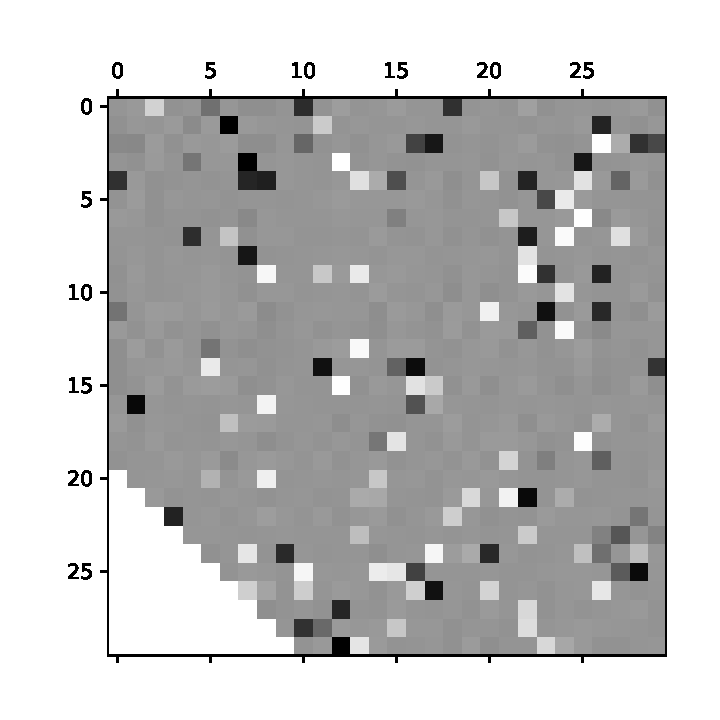
\includegraphics[width=.5\textwidth]{pics/chapter2/matrix.pdf}
    \caption{\small $30\times30$的模拟矩阵,左下角白色代表缺失值,图中灰度越深代表元素的绝对值越大,因此深黑色的点代表了离群值}
    \label{fig2.1}
\end{figure}

基于获得的高维低秩矩阵,我们主要比较以下算法:
对于$L_1$范数主成分分析,我们使用交替凸优化算法,记作ACP-$L_1$。
对于$L_2$范数主成分分析,采用了下面三种算法:
1)奇异值分解,该算法需要进行缺失值插补,这里我们使用均值插补法。记作SVD;
2)基于交替凸优化算法,但是更换损失函数为$L_2$范数,可以直接处理原始数据。记作ACP-$L_2$;
3)一种基于迭代加权$L_2$范数的估计方法\cite{srebro2003weighted},
通过将问题$P_1$损失函数加上随迭代变化的权重,可给$L_2$范数主成分分析带来一定的稳健性
,可以直接处理原始数据。记作IRLS(iteratively reweighted least squares)。

\subsubsection{实验结果}
令$\hat{\bm{X}} = \hat{\bm{A}}_{N \times M}\hat{\bm{F}}_{M \times N}$,我们比较因子残差
$\bm{E} = \hat{\bm{X}} -\bm{X}$。观察重构残差的平方的分布情况,
试验每一种算法作用在无干扰数据上和干扰后数据上的情况。

对于无干扰数据,每一种算法都具有很好的表现;
对于进行了缺失值和离群值模拟的数据,我们每组试验(给定$M$,$ N$)下均重复多次取平均值。图2.3给出了一个典型结果,
图中$N = 80, M=3$,缺失值和离群值比例均为$10\%$,进行了10次实验后重构残差的平方的分布情况,横轴表示残差平方,
纵轴表示平均频数。
可以看出ACP-$L_1$的重构残差表现最好。
\begin{figure}[H]
    \centering
    \begin{minipage}[t]{0.48\textwidth}
    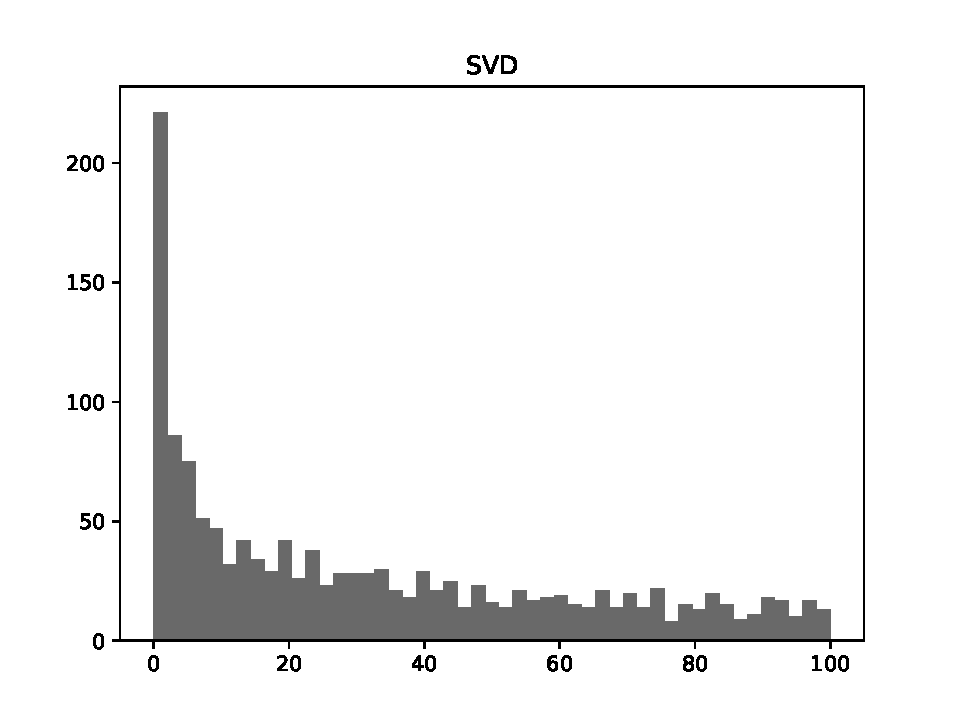
\includegraphics[width=8cm]{pics/lab1/svd.pdf}
    \end{minipage}
    \begin{minipage}[t]{0.48\textwidth}
    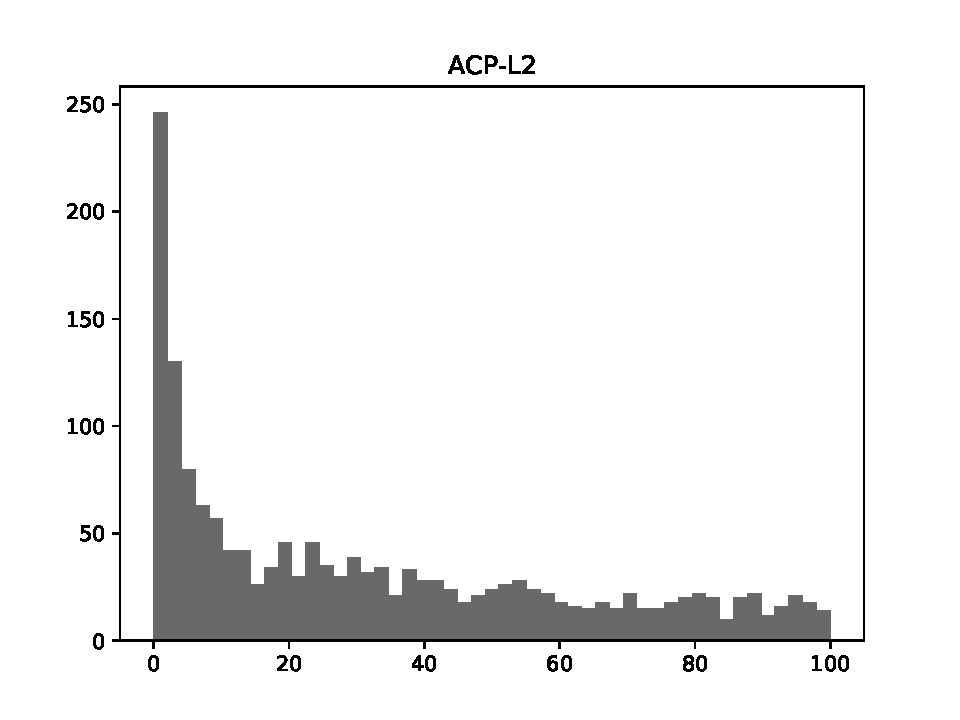
\includegraphics[width=8cm]{pics/lab1/acp-l2.pdf}
    \end{minipage}
    \begin{minipage}[t]{0.48\textwidth}
    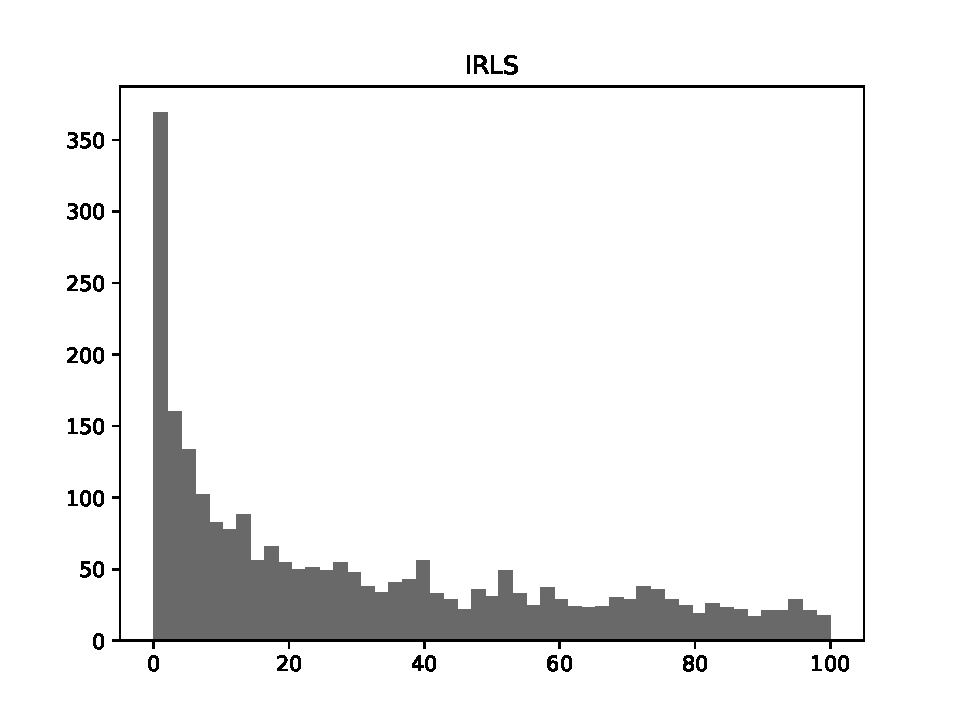
\includegraphics[width=8cm]{pics/lab1/IRLS.pdf}
    \end{minipage}
    \begin{minipage}[t]{0.48\textwidth}
    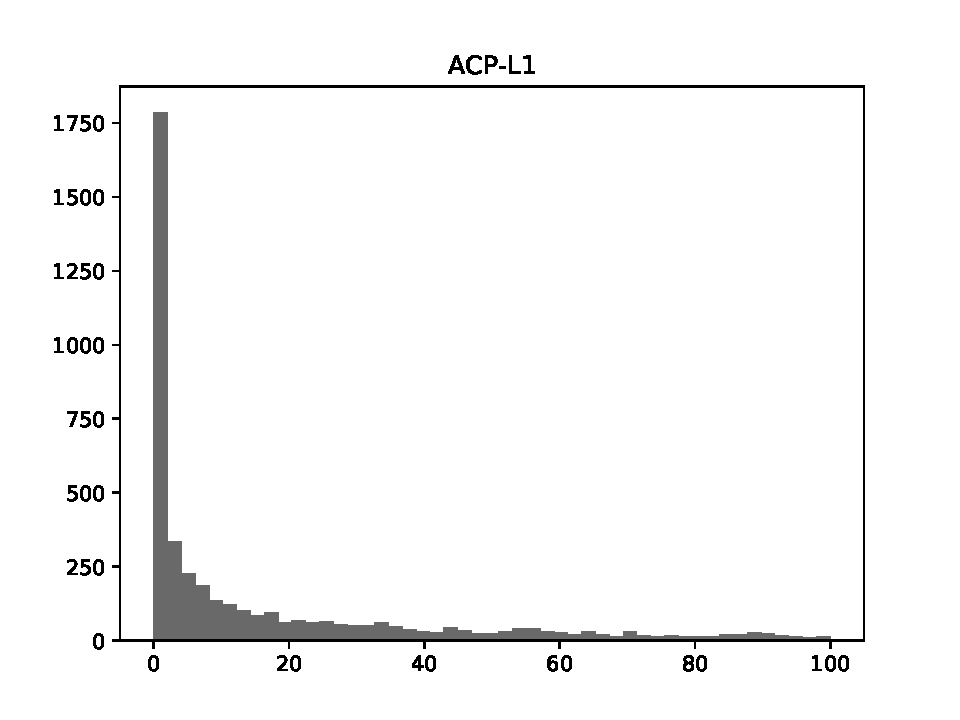
\includegraphics[width=8cm]{pics/lab1/acp-l1.pdf}
    \end{minipage}
    \caption{\small 几种方法重构残差对比}
\end{figure}

实验表明,$L_1$范数主成分分析相比$L_2$主成分分析法和其他基于$L_2$范数优化的方法相比具有更好的稳健性,
特别适合于处理具有大量离群值的数据。

\subsection{基于国内主要月度宏观经济数据的实证研究}
上一节我们阐述了$L_1$范数主成分分析方法,本节我们进行基于国内主要月度宏观数据的实证研究,来探究
使用$L_1$范数主成分分析用来代替$L_2$范数主成分分析进行近似因子模型估计的可行性。

数据方面将选择高维的国内主要月度宏观经济数据,该数据集包含众多的经济指标,其中许多经济指标
具有重尾分布,即意味着包含较多的离群值。并且该数据集在时间序列上不完整,一些经济指标的观测值缺失。

本实证研究采用扩散指数模型进行经济预测\cite{stock2002macroeconomic},近年来该模型已经得到了广泛的应用。
该预测模型依赖近似因子模型的因子得分估计作为关键自变量,本次研究将对比$L_2$范数和$L_1$范数主成分分析
下不同的因子得分估计在宏观经济指标预测中的表现。最后,将结合实证结果对$L_1$范数主成分分析在
本场合的应用提出一些建议。

\subsubsection{扩散指数模型}
令$y_t$为待预测经济变量$y$在时间$t$的水平,$\bm{X}_t$为
$p$维随机向量,假设$(X_t,y_t)$服从近似因子模型并且$\bm{X}_t$和$y_t$具有相依性,
若$\bm{X}_t, y_t$有$m$维共同因子$\bm{F}_t$,即
\begin{equation}
    \bm{X}_t = \bm{A}\bm{F}_t + \bm{e}_t
\end{equation}
则可以通过式\eqref{predict-factor-model}对$y_{t+h}$进行预测,
\begin{equation}\label{predict-factor-model}
    y_{t+h} = \bm{\beta}(L)\bm{F}_t + \bm{\alpha}(L)y_t + c + e_{t+h}
\end{equation}
其中滞后算子$\bm{\beta}(L)$反映了共同因子滞后项的影响,而
$\bm{\alpha}(L)$表示$y_t$自身的滞后项的影响。

我们取$h = 1$即可以得到向前一期的预测结果。而为了预测第$h\ (h > 1)$期变量水平,可以通过每次向前预测一期,将
该期预测值加入模型递归地向前预测。

\subsubsection{因子个数判定}
在进行因子分析前,我们需要判定因子个数,这方面国内外学者已经做了较多的研究
(Connor et al, 1993\cite{connor1993test};Bai and Ng, 2002\cite{bai2002determining};
Kapetanios et al, 2010\cite{kapetanios2010testing}
)。
本节采用Bai和Ng于2002年提出的确定静态因子个数的信息准则,该准则
平衡了模型的拟合优度和模型简约性。
在该信息准则下,我们的因子个数需要最小化
\begin{equation}\label{number}
    IC(m) = \ln(V(\hat{\bm{A}}, \hat{\bm{F}})) + mG(p, T)
\end{equation}
其中$V(\hat{\bm{A}}, \hat{\bm{F}})$为因子残差平方和除以$pT$。
而$G(p,T)$为一惩罚函数,该函数使得在$p,\ T \rightarrow \infty$时
$G(p, T) \rightarrow 0$且$min(p, T)G(p,T) \rightarrow \infty$。
参考Bai和Ng文中建议,本节实证研究中选择
$$
    G(p, T) = (\frac{p + T}{pT})\ln(\frac{pT}{p + T})
$$
构造信息准则。

需要说明的是由于使用交替凸优化算法求解$L_1$主成分分析需要$m$已知,
为与$L_2$主成分分析公平比较,我们利用$L_2$主成分分析确定因子个数。

\subsubsection{数据说明}
本次实证研究数据来自EPS数据平台——中国宏观经济数据库。

我们选择了从1999年9月至2019年6月主要公开月度宏观经济指标,主要包括了工业(重工业增加值、轻工业增加值、铁矿石原产量、工业企业利润总额等)、
运输和邮电业(客运总量、货运总量、邮电业务总量等)、
能源(原油生产总量、发电量、原煤产量等)、
国内贸易(烟酒消费品零售总额、日用品类零售总额、粮油食品类零售值、服装纺织品类零售值等)、
固定资产投资(第一产业固定资产投资、建筑安装工程投资、设备工具购置投资等)、
房地产开发业(住宅投资完成额、办公楼投资完成额、建筑工程投资额、安装工程投资额等)、
对外经济贸易(对外承包工程营业额、纺织品出口金额、大豆进口量、原油进口量等)、
财政(国家债务收入、企业亏损补贴、一般公共服务支出、社会保障和就业支出等)、
金融(货币供应量、股票成交额、基金份额、人民币汇率等)、
保险(财产险保费收入、人身险保费收入、财产险保费支出、保险业投资等)、
就业与社会保障(城镇新增就业人数、城镇职工基本养老保险基金收入、医疗保险基金支出等)等共11个类别,总计120个指标的月度时间序列。

另外,我们还选择了一些景气指数,它们在本次实证研究中既可用来作为待预测的变量,也可用来做预测变量形成对照组。
我们这里选择了制造业采购经理指数、非制造业采购经理指数、消费者预期指数、消费者满意指数
和消费者景气指数等。

\begin{figure}[H]
    \flushleft
    \begin{minipage}[t]{1\textwidth}
    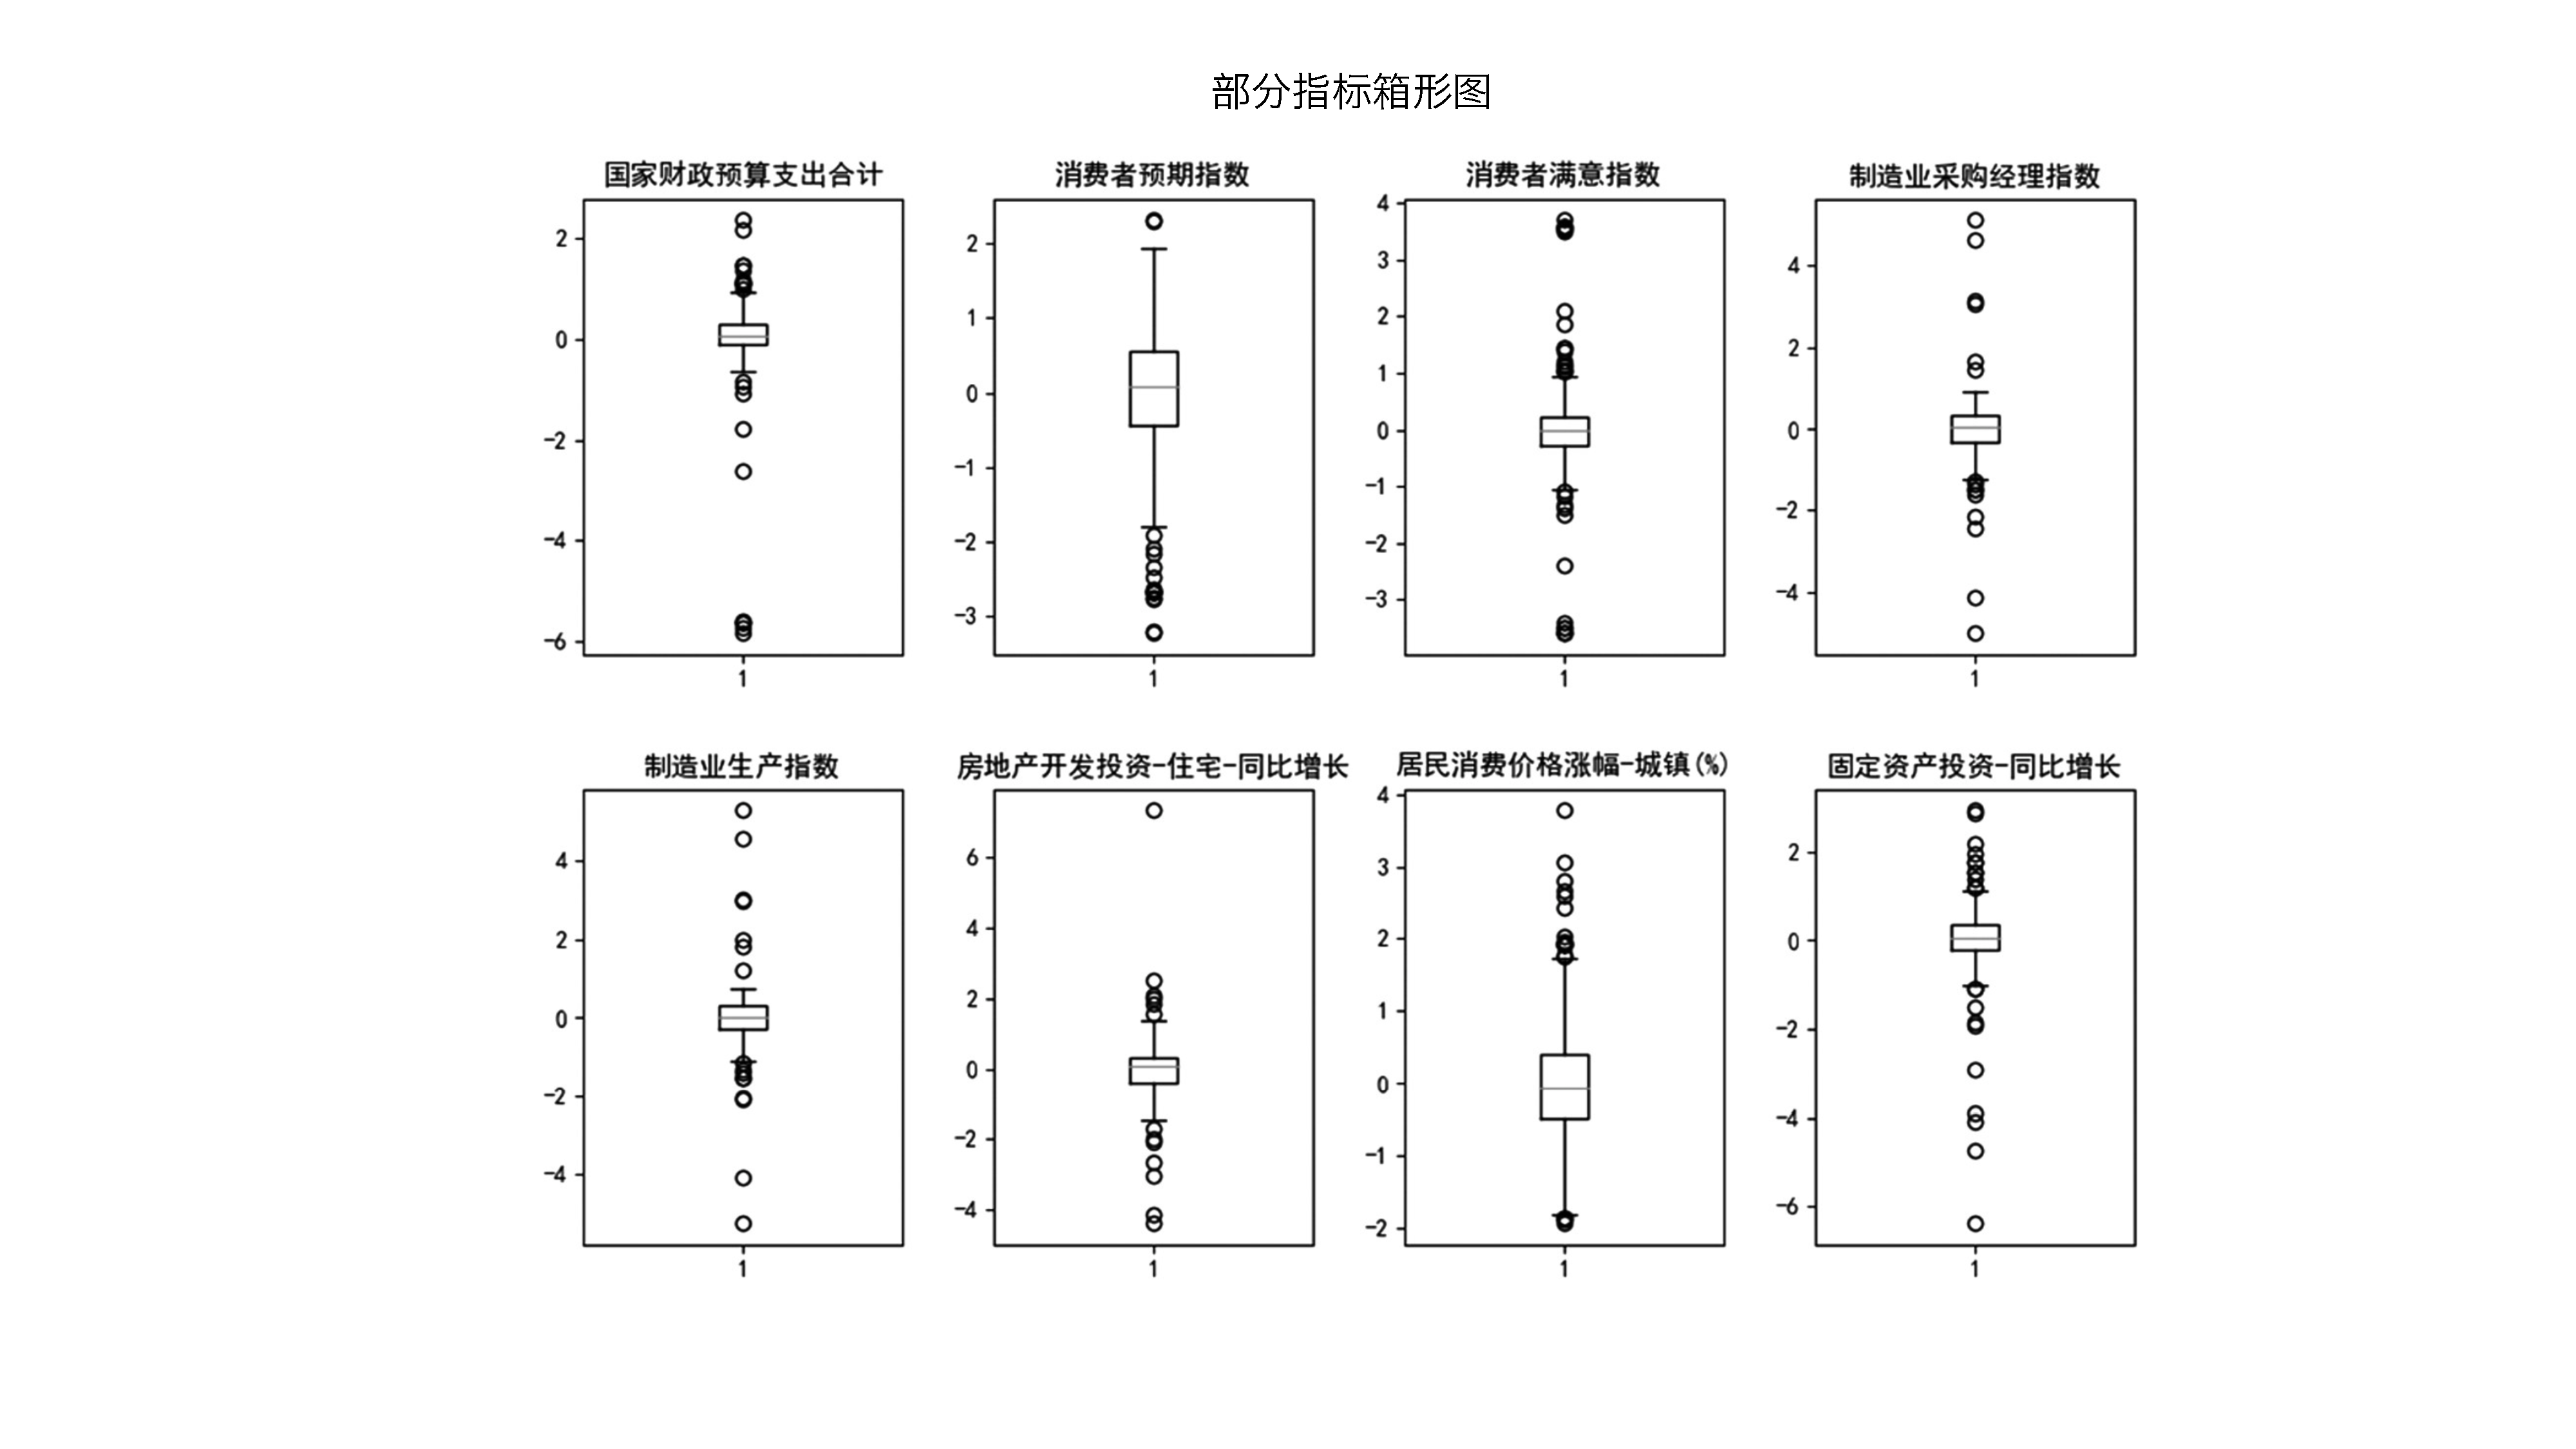
\includegraphics[width=16cm]{pics/chapter2/box.pdf}
    \end{minipage}
    \begin{minipage}[t]{1\textwidth}
    \centering
    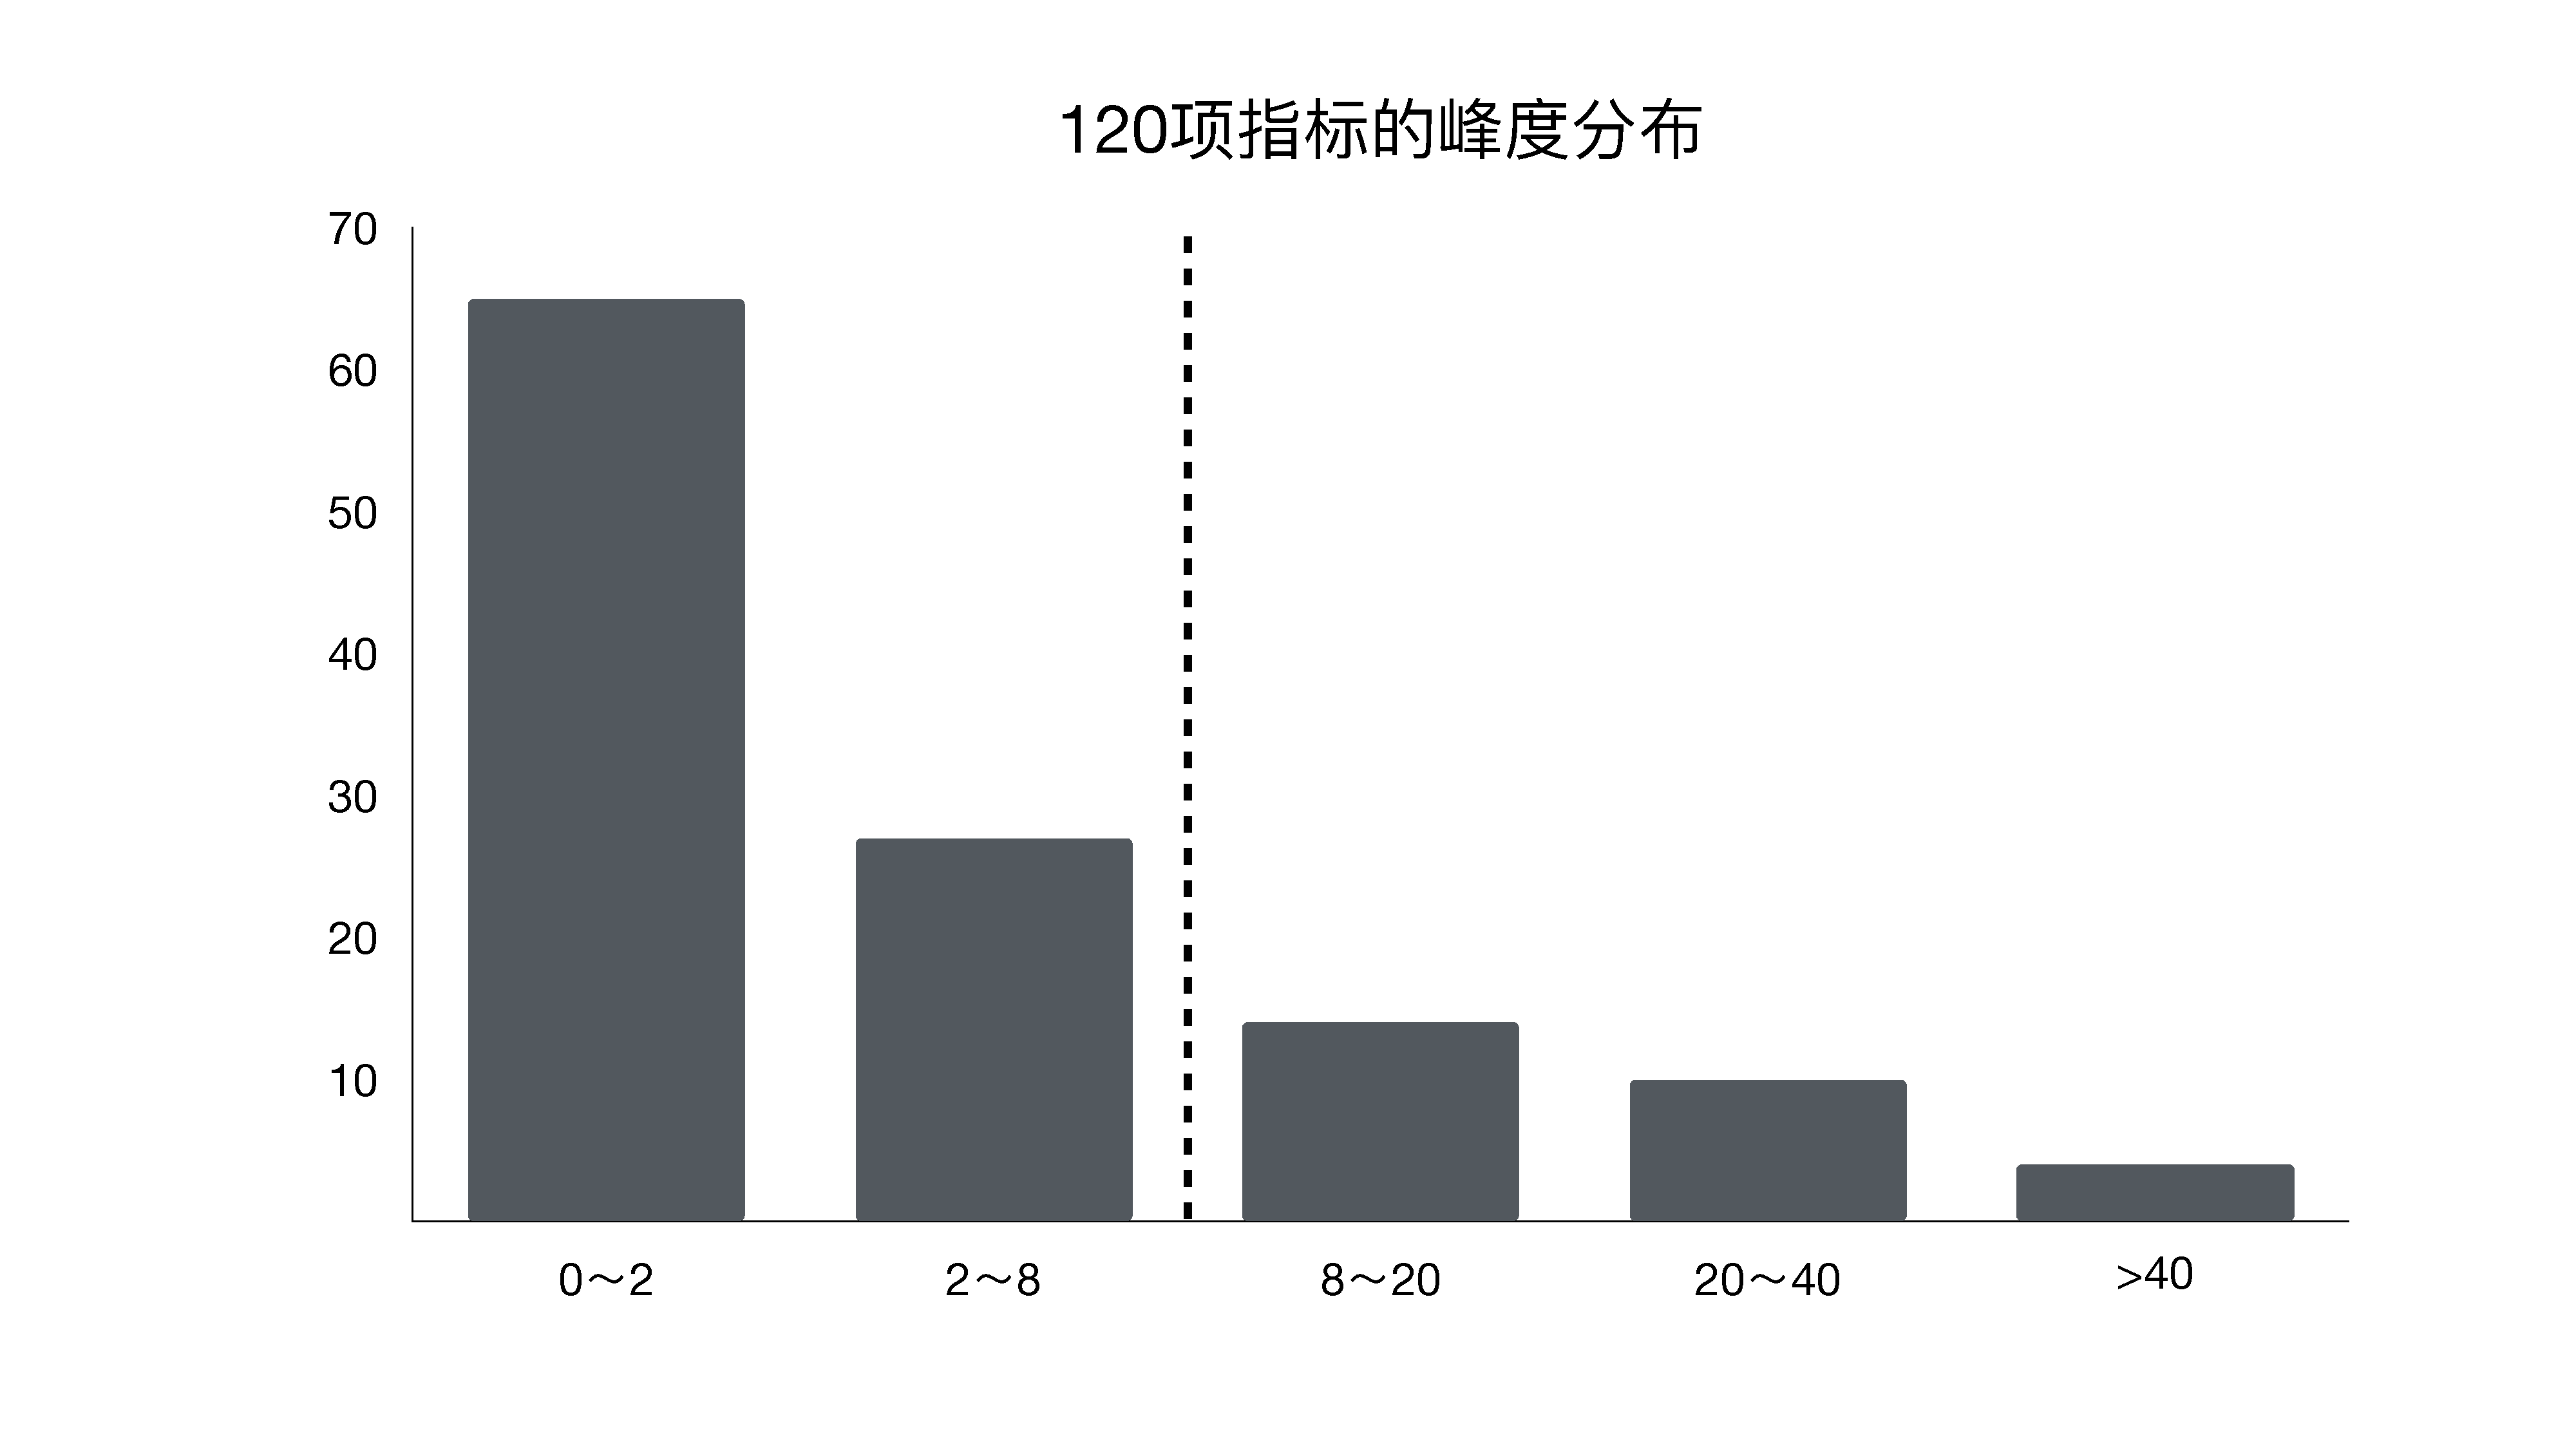
\includegraphics[width=12cm]{pics/chapter2/skew.pdf}
    \end{minipage}
    \caption{\small 部分指标的箱形图和各经济指标的峰度分布情况}
    \label{desc}
\end{figure}

由于某些指标曾多次改变统计口径、统计频率等原因,这些数据中包含许多的缺失数据。
另外,在1999~2019年这20年间,中国经济经历了数次重大外部冲击,许多经济指标中含有大量离群值(见图\ref{desc}),
从各指标的经验分布的峰度值(一般峰度大于8就被认为是重尾,8是自由度为5的$t$分布的峰度值)来看,许多经济指标的分布存在分布重尾的现象。

在预处理阶段,我们对不平稳数据进行一阶差分;之后所有数据均进行标准化(所有观测减去样本均值,然后除以样本标准差)处理,我们不剔除任何离群值;
另外,对于缺失数据的情况,在进行$L_2$主成分分析时对原始数据进行插补,插补方法是对已有数据拟合ARMA模型
并根据估计得到的模型填补对应缺失数据。

下面介绍两组因子的主成分估计量的获得:首先进行$L_2$主成分分析并根据\eqref{number}选择最合适的因子个数
(本组数据得出最佳因子个数为8);接下来将$L_2$主成分估计的因子载荷矩阵作为交替凸优化算法$\bm{A}^0$的初始值,
然后求解得到$L_1$因子载荷。根据\eqref{factor}得出两组因子得分的估计:我们称为$L_1$因子和$L_2$因子。

\subsubsection{实证结果}

将得到的$L_1$因子和$L_2$因子看作$m$维随机向量的一组时间序列,根据\eqref{predict-factor-model}建立预测模型。
对预测结果的评价,下面选取了三种指标:MSE、MAE和MPAE,其计算方法如下($e_t$为$t$时期的预测误差)。
\begin{equation}
    \begin{array}{clr}
        \text{MSE} &= \frac{1}{n}\sum_{t=1}^n e_t^2 \\
        \text{MAE} &= \frac{1}{n}\sum_{t=1}^n |e_t| \\
        \text{MPAE} &= \frac{1}{n}\sum_{t=1}^n |e_t / y_t| \\
    \end{array}
\end{equation}

由于景气指数反映了经济中多方面特征,因此也可以将几种景气指数的时间序列作为预测变量,也根据\eqref{predict-factor-model}建立预测模型。
我们把$L_2$因子的三种平均误差指标作为基准,记录$L_1$的对应误差和它的比,作为对照我们这里将景气指数模型的预测情况也进行展示。

对于每一指标,我们选取前24月观测作为预测数据,比较下$h$期的预测值和其真实值。我们采用滑动窗口预测,每次记录相应的预测误差,最终记录预测误差的
平均情况。

\begin{figure}[H]
    \centering
    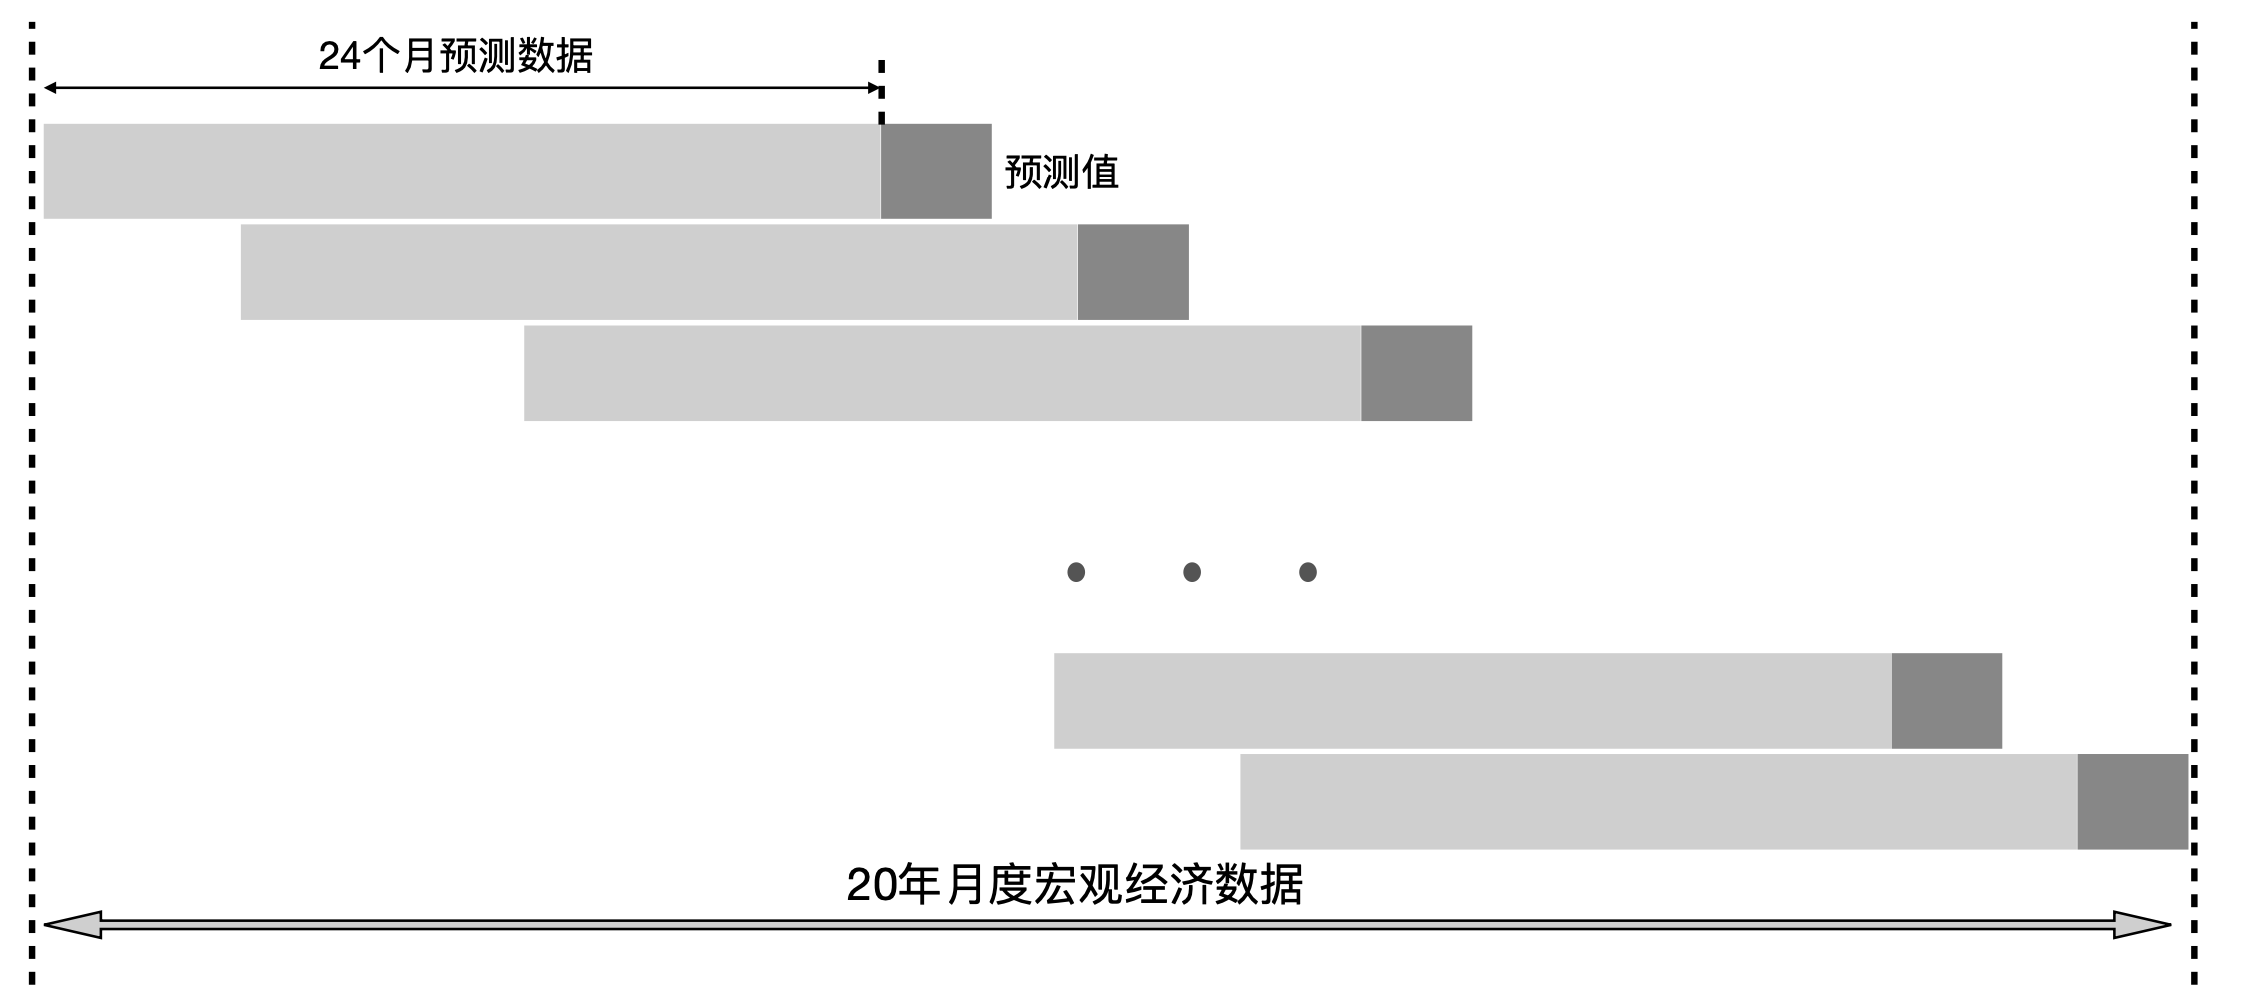
\includegraphics[width=15cm]{pics/chapter2/predict.png}
    \caption{\small 滑动窗口预测示意图}
    \label{desc}
\end{figure}

表\ref{outcome1}、表\ref{outcome2}和表\ref{outcome33}分别对应了$h = 1, 3, 6$,分别对应下一个月、下一个季度和半年后的预测情况。其中
IM为景气指数模型的预测情况;L1\ PCA为$L_1$因子的预测情况。表格中带有*号标记的变量名称表示对于该指标,使用$L_1$主成分估计的因子在三种预测误差
测度中有两种小于$L_2$主成分估计的因子预测。

\begin{table}[H]
    \small
    \caption{向前一个月预测结果}
    \label{outcome1}
    \centering
    \begin{tabularx}{\textwidth}{lXXXXXX}
    \toprule
                     &  MSE(L1 PCA) &  MSE(IM) &  MAE(L1 PCA) &  MAE(IM) &  MPAE(L1 PCA) &  MPAE(IM) \\ \midrule
    消费者满意指数*     & 0.81            & 1.49        & 0.87            & 1.67        & 0.43             & 1.55         \\
    工业生产者出厂价格指数* & 0.70            & 1.98        & 0.75            & 1.54        & 0.96             & 1.60         \\
    货币供应量M2*      & 0.76            & 1.25        & 0.90            & 1.19        & 0.45             & 0.97         \\
    固定资产投资总额*  & 0.89            & 1.03        & 0.97            & 0.99        & 0.81             & 1.32         \\
    房地产开发投资总额* & 0.79            & 0.98        & 0.95            & 1.00        & 0.91             & 1.20         \\
    社会消费品零售总额* & 0.84            & 1.25        & 0.87            & 1.12        & 0.45             & 1.17         \\
    制造业采购经理指数    & 1.24           & 1.69        & 1.06            & 1.43        & 0.90             & 1.50         \\
    住宅新开工面积总数*  & 0.89            & 2.40        & 0.85            & 1.98        & 0.45             & 2.22         \\
    股票流通市值*      & 0.99            & 3.99        & 0.98            & 2.84        & 0.81             & 4.51         \\
    消费者信心指数*     & 0.93            & 1.01        & 0.98            & 0.99        & 0.98             & 1.56         \\ \bottomrule
    \end{tabularx}
\end{table}

\begin{table}[H]
    \small
    \centering
    \caption{向前三个月预测结果}
    \label{outcome2}
    \begin{tabularx}{\textwidth}{lXXXXXX}
    \toprule
                 &  MSE(L1 PCA) &  MSE(IM) &  MAE(L1 PCA) &  MAE(IM) &  MPAE(L1 PCA) &  MPAE(IM) \\ \midrule
                 消费者满意指数*     & 0.85            & 1.16        & 0.95            & 1.22        & 1.32             & 1.93         \\
    工业生产者出厂价格指数* & 0.97            & 1.39        & 0.97            & 1.20        & 0.93             & 1.12         \\
    货币供应量M2       & 1.08            & 1.20        & 1.05            & 1.44        & 0.66             & 1.70         \\
    固定资产投资总额*  & 0.98            & 1.11        & 0.98            & 1.28        & 0.82             & 0.89         \\
    房地产开发投资总额* & 0.91            & 0.94        & 0.92            & 1.12        & 0.66             & 0.99         \\
    社会消费品零售总额* & 0.63            & 1.12        & 0.85            & 0.99        & 1.26             & 1.05         \\
    制造业采购经理指数    & 1.26            & 1.10        & 1.10            & 1.30        & 1.04             & 1.72         \\
    住宅新开工面积总数   & 0.82            & 1.62        & 1.12            & 1.78        & 1.04             & 1.23         \\
    股票流通市值   & 0.99            & 1.98        & 1.00            & 1.50        & 1.04             & 1.91         \\
    消费者信心指数*     & 0.99            & 1.35        & 0.96            & 1.02        & 0.94             & 1.17         \\ \bottomrule
    \end{tabularx}
\end{table}

\begin{table}[H]
    \small
    \centering
    \caption{向前六个月预测结果}
    \label{outcome33}
    \begin{tabularx}{\textwidth}{lXXXXXX}
    \toprule
                 &  MSE(L1 PCA) &  MSE(IM)&  MAE(L1 PCA) &  MAE(IM) &  MPAE(L1 PCA) &  MPAE(IM) \\ \midrule
                 消费者满意指数*     & 0.91            & 1.20        & 0.93            & 1.12        & 0.68             & 1.81         \\
    工业生产者出厂价格指数* & 1.00            & 1.30        & 0.94            & 1.18        & 0.79             & 1.77         \\
    货币供应量M2      & 0.84            & 1.12        & 1.06            & 1.05        & 1.46             & 1.08         \\
    固定资产投资总额*  & 0.88            & 1.43        & 0.94            & 1.29        & 0.93             & 1.85         \\
    房地产开发投资总额* & 0.90            & 1.01        & 0.91            & 1.12        & 0.73             & 1.07         \\
    社会消费品零售总额* & 0.64            & 1.39        & 0.79            & 1.20        & 1.30             & 1.34         \\
    制造业采购经理指数   & 1.46            & 1.40        & 1.20            & 1.32        & 1.45             & 1.82         \\
    住宅新开工面积总数*  & 0.85            & 1.50        & 0.96            & 1.36        & 0.70             & 1.02         \\
    股票流通市值   & 0.98            & 2.24        & 1.01            & 1.96        & 1.28             & 2.98         \\
    消费者信心指数*     & 0.99            & 1.48        & 0.98            & 1.19        & 0.97             & 1.70         \\ \bottomrule
    \end{tabularx}
\end{table}

从结果中可以看出,$L_1$主成分估计的因子有着良好的预测表现。在对下一个月的预测中,其预测准确度略高于$L_2$主成分估计;
在对下一个季度和半年后的预测中,两者的表现类似。
通过和景气指数模型的对比来看,使用任何一种因子估计的预测总体表现都更准确,这也验证了Stock等人的结论\cite{stock2002forecasting}。
我们可以做出结论,$L_1$主成分分析同样可以用来作为近似因子模型的估计,并且应用于扩散指数模型进行宏观经济预测。这意味着
在处理数据有缺失、不满足高斯分布假设时,可以直接使用$L_1$主成分分析来估计因子模型,它不仅仅能提供更好的稳健性,
同时也拥有很好的预测效果。

\subsection{本章小结}
本章首先简要介绍了因子模型的基础理论,包括了正交因子模型、动态因子模型和近似因子模型的基本概念和模型参数的估计方法。
正交因子模型主要通过主成分分析法来估计,而动态因子模型估计较为困难,常常估计其静态形式。
我们介绍了近似因子模型的主成分估计,在这里是作为一种非参数估计,
而主成分估计得出的因子得分可以很好地应用于宏观经济预测。

基于以上事实,结合宏观经济数据的一些重尾和缺失特征,我们希望在进行主成分分析时作稳健性上的改进,故
提出了采用$L_1$范数的主成分分析代替$L_2$主成分分析来估计模型。我们对$L_1$主成分分析的问题进行了表述,介绍了
一种交替凸优化算法并给出其实现步骤,
并通过模拟实验论证了$L_1$主成分分析
的确具有更好的稳健性。

最后,为了验证$L_1$主成分分析能否代替$L_2$主成分分析作为近似因子模型的估计。我们基于国内的一组月度宏观经济数据作了实证
研究,将两种不同的主成分估计引用在扩散指数模型的预测上。实证研究的结果表明,因子模型的$L_1$主成分估计量同样适用于
进行宏观经济预测,具有良好的预测效果。这启发我们在处理宏观经济数据时,可以充分利用$L_1$主成分分析手段来加强
分析的稳健性。

本章的研究成果已经于2019年进行了发表\cite{孔新兵2019高维}。近期又有一些理论上的新进度,如Chen Liang等于2021年(Econometrica, to appear)在理论上证明了
$L_1$主成分分析进行因子分析的相合性。

$L_1$主成分分析在计算开销上大许多,我们介绍的交替凸优化算法在实证研究中也体现出来这一缺点。在本文后续研究中,
我们将对交替凸优化算法的改进做一些尝试。
   \section{最小绝对值回归的性能研究}\label{chapter3}

本文的主题是稳健$L_1$范数主成分分析方法在宏观经济中的应用问题研究。
$L_1$范数是最常用的几种重要范数之一,它在数值计算、统计学、运筹学、
机器学习等领域有着极为重要的应用。在统计学研究中,已经基于$L_1$范数发展出了许多
稳健统计方法\cite{dodge2012statistical},主要是利用$L_1$范数的良好统计性质。

$L_1$范数稳健方法在计量经济学中一个重要应用是最小绝对值回归(
Davis and Dunsmuir, 1997\cite{davis1997least};
Ellis et al, 1998\cite{ellis1998instability};
Pollard, 1999\cite{pollard1991asymptotics};
Dasgupta and Mishra, 2004\cite{dasgupta2004least};
Li and Arce, 2004\cite{li2004maximum}
)。
最小绝对值回归最早提出是为了弥补最小二乘法的不足。
使用最小二乘法建立的线性回归模型虽然具有较好的解释性,
但是高斯——马尔可夫条件对模型变量的分布有正态性的要求。因此直接使用最小二乘法来建立模型,往往
对原始数据的分布情况要求高。即使变量满足了正态分布,但在模型系数估计时,样本中离群值的存在对
模型的系数估计效果有很大影响。

在宏观经济实证研究中,经济变量一般
不能够服从正态分布,而因受到经济冲击呈现出重尾的特征。对这样的原始数据不能够通过最小二乘法直接建模,
因此常常在回归中剔除异常点,使得经济变量接近正态分布,然而代价是有可能损失较多有价值的信息。

采用最小绝对值回归,是更加稳健的做法。实质上它就是中位数回归,模型的系数也具有很好的解释意义,
已经广泛应用在研究居民收入\cite{dasgupta2004least},生存分析\cite{ying1995survival},
并且在金融数据分析领域有着广泛的应用\cite{dasgupta2004least}。
在模型的拟合上,最小绝对值回归对离群值不敏感,具有相当的稳健性,因此可以很好处理重尾的宏观经济变量。

高维宏观经济数据,往往包含了维数众多的经济变量,并且样本数量往往非常大,
此时如果想要直接使用最小绝对值回归,在求解时就
需要解决变量维数和约束数量很高的线性规划问题,因此计算的开销很高。

最小绝对值回归在计算上的复杂性在一定程度上限制了它的应用。
一直以来,普遍的加速最小绝对值回归的方法都尝试使用平滑化方法来近似最小绝对值回归的目标函数,
避免直接使用原目标函数。然而,替换目标函数,可能会影响估计量的一致性从而
影响最小绝对值回归模型的解释性。

但是近年来随着统计学和机器学习领域
对$L_1$范数的研究逐渐深入,不断有新的算法尝试解决这个问题。
本章将介绍最小绝对值回归的两种较新的估计算法,一种是基于聚类——迭代拆解的算法;
另一种是基于替代变量的牛顿迭代方法,两种算法基于不同的出发点,
都在一定程度上对解决最小绝对值回归问题做了优化。

我们在第\ref{chapter2}章中介绍了求解$L_1$主成分分析的交替凸优化算法,
该算法简洁直观,并且交替迭代的子凸优化问题可以有最优解。其中\eqref{subpro}和\eqref{subproabs}
在交替凸优化算法中我们采用线性规划来求解,
但是对于高维宏观经济数据而言,维数$p$和样本量$n$都非常大,由于交替凸优化算法中大量采用线性规划法求解,
使得计算开销非常大。而在许多场合,我们常常希望快速得到近似因子用于进一步分析,这就
对$L_1$主成分分析提出了计算性能上的要求。本章研究最小绝对值回归的性能优化算法,
有助于我们改进交替凸优化算法的尝试,对本课题的研究有着重要意义。


\subsection{简介}
\subsubsection{最小绝对值回归的稳健性}

$L_2$范数最优化问题最常见的是最小二乘法。
最小二乘法的优点很多,这里不赘述。尽管在求解大部分问题时用最小二乘估计求解可以得到比较令人满意
的效果, 但最小二乘法也存在一些局限性, 比如, 当收集的数据较少或者具有较多的缺失数据
并且数据中夹杂有异常点时, 用最小二乘法所得的结果就令人难以接受, 在此情况下应用所得到的回归方程或模型进行预测或者拟合时, 
则预测或拟合的精度不可靠。正因为最小二乘法对数据中的异常值十分敏感,
当数据中具有较多离群值时,通过最小二乘、PCA和SVD方法,得到的估计结果也会受到较大影响。

设$\bm{X} = (X_1, X_2, ..., X_p)^T$为一$p$维随机向量,$Y$为响应变量,$\bm{\beta}$为回归系数。
假设我们观察到$i.i.d. $样本$\bm{X}_{n\times p} = (\bm{x}_1, \bm{x}_2, ..., \bm{x_n})^T$和$\bm{Y}_{n\times1}=
(y_1, ..., y_n)^T$,我们一般使用$\bm{\beta}$
的最小二乘估计量
\begin{equation}\label{l2loss}
\hat{\bm{\beta}} = \underset{\bm{\beta}}{\operatorname{arg\ min}} \sum_{i=1}^n\|y_i - \bm{x}^T_i\bm{\beta}\|_{L_2}
=\underset{\bm{\beta}}{\operatorname{arg\ min}} \sum_{i=1}^n(y_i - \bm{x}^T_i\bm{\beta})^2
\end{equation}
在稳健统计中,我们经常使用其他的目标函数,例如使用$L_1$范数来代替$L_2$,

\begin{equation}\label{l1loss}
\hat{\bm{\beta}} = \underset{\bm{\beta}}{\operatorname{arg\ min}} \sum_{i=1}^n\|y_i - \bm{x}^T_i\bm{\beta}\|_{L_1}
=\underset{\bm{\beta}}{\operatorname{arg\ min}} \sum_{i=1}^n|y_i - \bm{x}^T_i\bm{\beta}|
\end{equation}

通常使用$L_1$范数在线性回归中可以有效避免离群值造成的干扰。
如图\ref{fig2.1}所示,在简单的线性模型的拟合中,出现一个离群值就可以导致最小二乘法拟合出现明显的偏差;
    而含有较多离群值时最小二乘法拟合变得很不可靠;而采用$L_1$范数则具有相当稳健性。
\begin{figure}[H]
    \centering
    \begin{minipage}[t]{0.48\textwidth}
    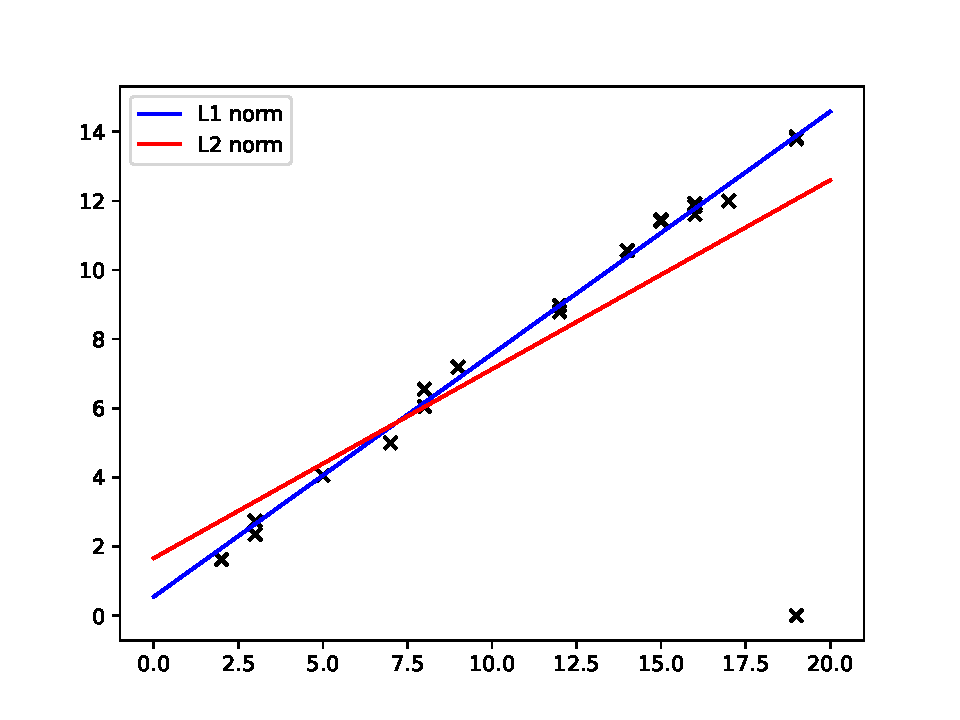
\includegraphics[width=8cm]{pics/chapter2/l1-l2-diff2.pdf}
    \end{minipage}
    \begin{minipage}[t]{0.48\textwidth}
    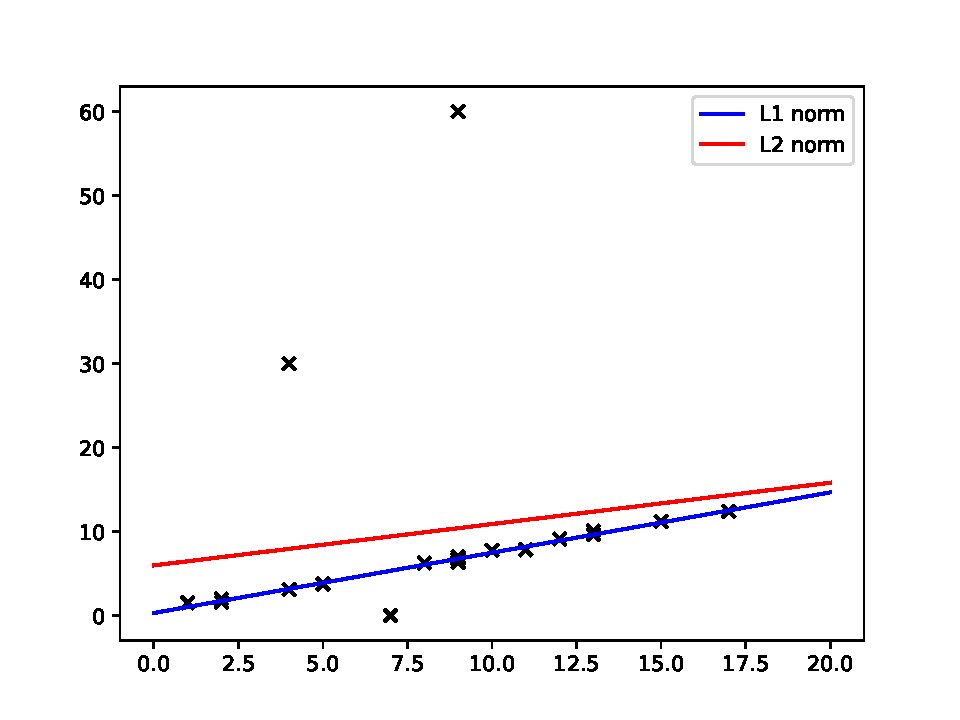
\includegraphics[width=8cm]{pics/chapter2/l1-l2-diff.pdf}
    \end{minipage}
    \caption{\small 数据含有离群值时最小二乘和最小绝对值回归的拟合情况}
    \label{fig2.1}

\end{figure}

我们使用$L_1$目标函数来估计$\bm{\beta}$,则其中$\bm{\beta}^*$为最小绝对值回归系数,$e$为一随机噪声,
可以写出最小绝对值回归的一般形式
\begin{equation} \label{l1losstotal}
    \begin{split}
    Y &= \bm{X}^T\bm{\beta}^* + e\\
    \bm{\beta}^* &= \underset{\bm{\beta}\in \mathbb{R}^{p}}{\operatorname {arg\ min}}
    \mathbb{E}|Y - X\bm{\beta}|.
    \end{split}
\end{equation}

\subsubsection{最小绝对值回归的估计方法}
对于\eqref{l1loss},它是一个凸优化问题,但是其不具备显式解,一般求它的数值解。但是其目标函数在$\bm{0}$点不可导,
因此不能直接使用使用梯度下降法,一般来说,该问题
的全局最优解可以通过求解下面的线性规划问题得到:
$$
    \underset{\bm{\beta}, \bm{t}}{\operatorname{min\ }} 1^T \bm{t}
$$
$$
    s.t. -\bm{t} \leq \bm{X}_{n\times p}\bm{\beta}_{p\times1} - \bm{Y}_{n\times 1} \leq \bm{t}
$$
目前对于线性规划问题已经有了比较成熟的解决方法,主要通过单纯形法或者内点法求解,后者的时间复杂度可以控制在多项式时间,
然而,一般而言,当$n$和$p$均很大时,上述线性规划问题面临很高的变量和约束维数,计算速度仍较慢。

由于$L_1$范数的目标函数在机器学习领域的大量使用,已经产生了一些光滑化方法,做法是用一个接近$L_1$的目标函数来替代它,
用来替代的函数往往处处可导,因而可以使用梯度下降法求解。
典型的代表就是使用Huber’s M统计量近似$L_1$范数目标函数\cite{lucas1997robustness},
\begin{equation*}
    \rho(e) = \left\{
        \begin{array}{clr}
            \frac1{2}e^2,\ |e| \leq \gamma \\
            \gamma |e| - \frac1{2}\gamma ^2 ,\ |e| > \gamma
        \end{array}
    \right.
\end{equation*}
其中$\gamma$为某一正数,该问题可以转化为一个二次规划问题求解。

\subsection{聚类——迭代拆解算法}
近年来针对最小绝对值回归的性能研究发展出了除了光滑化目标函数之外的方法,可以在不改变目标函数的情况下,
通过寻求新的优化方法进行求解。这样一来,可不改变最小绝对值回归估计量的统计性质。
这里介绍Park等人于2019年提出的一种基于聚类——迭代拆解算法的最小绝对值回归求解方法\cite{park2021optimization}。

\subsubsection{聚类——迭代拆解算法说明}
聚类是一种在机器学习中常见的做法,就是按照某种给定的规则,将特征接近的样本点归类到一起。
聚类——迭代拆解算法的提出受到以下事实的启发:
1)优化问题面临的数据集规模庞大,其中许多的样本点在进行参数估计时的贡献很接近;
2)如果对相似的样本点进行聚类,提炼该聚类中的信息,避免每个样本点都进入计算,那么就会大大减小问题的规模;
3)假设在聚类后构造的新数据集上不能接近问题的最优解,那么就拆解当前的聚类,在新聚类上进行计算,
聚类个数有限,因此最坏情况下相当于直接求解原问题;

采用聚类——迭代拆解算法求解某个优化问题的前提如下:1)必须能够提出一种规则来对样本点聚类;
2)必须找到合适的聚类和拆解聚类的标准;
3)需要在聚类后构造的新数据集上明确定义新的优化问题;
4)能够判定当前解是否接近最优解。

\subsubsection{优化最小绝对值回归}
算法3.1给出了任何一个聚类——迭代拆解算法的主要步骤,注意算法3.1必然在某处停止,
因为每次不断拆解聚类,当聚类个数$|K^{t}|= n$时,相当于计算原问题,此时算法终止。
\begin{table}[H]%%%%%%开始表格
    \centering%把表居中
    \begin{tabular}{{p{0.9\columnwidth}}}%三个c代表该表一共三列,内容全部居中
    
    \toprule%第一道横线 表头
    {\heiti 算法} {\bf3.1} 聚类——迭代拆解算法(Aggregate and Iterative Disaggregate, AID) \\
    \midrule%第二道横线 符号+解释+单位 中间用&隔开
    输入:原始数据集$\bm{X}_{n\times p}$,样本点的下标集合${I} = \{1, 2, ..., n\}$,
    数据的特征下标集合${J} = {1, 2, ..., p}$,原优化问题$P$。\\
    初始化:对原始数据集$\bm{X}$聚类,然后按某种规则产生新的优化数据集$\bm{X}^{(1)}$。 \\
    对于$t = 1, ..., \tau$:\\
        记${C}^{(t)} = \{{C}_1^{(t)}, ..., C_K^{(t)}\}$为聚类的集合, $K^{(t)} = \{1, ..., |K^{(t)}|\}$为当前聚类的下标,
        \\
        1.根据当前聚类情况${C}^{(t)}$,构造新的数据集$\bm{X}^{(t)}$,求解相应的优化问题${P}^{(t)}$; \\
        2.检查解$\bm{s}^{(t)}$是否达到最优条件;\\
        3.如果不满足条件,拆解当前聚类。
        \\
    \bottomrule%第三道横线
    \end{tabular}
\end{table}%%%%%%结束表格

改写\eqref{l1loss}的目标函数,
\begin{equation}\label{l1loss2}
\xi^* = \underset{\bm{\beta} \in \mathbb{R}^{p}}{\operatorname{min}} 
\sum_{i \in I}|y_i - \sum_{j \in J}x_{ij}\bm{\beta}_j|
\end{equation}

首先给出聚类方法。给定$|K^{(0)}|$为目标聚类个数,初始化$C^{(0)} = \{C_1^{(0)}, C_2^{(0)}, ..., C_K^{(0)}\}$,
我们可以使用任意的聚类方法进行初始化。接下来给出如何根据聚类来产生新的数据集,
对于在任一迭代周期内产生的聚类$C^{(t)}_k, k = 1, ..., K^{(t)}$,取
\begin{equation*}
    x_{kj}^{(t)} = \frac{\sum_{i \in C_k^{(t)}}x_{ij}}{|C_k^{(t)}|},\ j \in J \  
    \text{并且} \
    y_{k}^{(t)} = \frac{\sum_{i \in C_k^{(t)}}y_i}{|C_k^{(t)}|}
\end{equation*}

对于每一个不同的聚类需要给出一个权重来区分信息量不同的聚类,因此在新的数据集上,我们求解下面的问题
\begin{equation}\label{clusterl1}
    F^{(t)} =\underset{\bm{\beta}^{(t)} \in \mathbb{R}^{p}}{\operatorname{min}} 
    \sum_{k=1}^{K^{(t)}}|C_k^{(t)}||y_k^{(t)} - \sum_{j \in J}x_{kj}^{(t)}\bm{\beta}_j^{(t)}|
\end{equation}
容易发现,任何\eqref{clusterl1}的可行解都是\eqref{l1loss2}的可行解。
记$\hat{\bm{\beta}}^{(t)}$为\eqref{clusterl1}的解,在每次迭代,我们计算此时的原目标函数的取值
\begin{equation}
    \xi^{(t)} = \sum_{i \in I} |y_i - \sum_{j \in J}x_{ij}\hat{\bm{\beta}}_j^{(t)}|
\end{equation}

接下来给出拆解聚类的准则:设$t$步的聚类集合为$C^{(t)}$,该步解为$\hat{\bm{\beta}}^{(t)}$,
对于$k = 1, ..., K^{(t)}$,计算$\theta_i = y_i - \sum_{j \in J}x_{ij}\hat{\bm{\beta}}_j^{(t)}$,

1)若对于任意$i \in C_k^{(t)}$,$\theta_i$有相同的符号,那么该聚类$C^{(t)}_k$将保留到下次迭代,即$C^{(t+1)} \leftarrow C^{(t+1)}\bigcup C^{(t)}_k$,见图
\ref{aid-demo};

2)若不满足上述条件,那么根据$\theta_i$符号异同,将$C^{(t)}_k$分成两个集合,$C_{k+}^{(t)} = \{i \in C_k^{(t)} | \theta_i > 0\}$ ,
$C_{k-}^{(t)} = \{i \in C_k^{(t)} | \theta_i < 0\}$,见图\ref{aid-demo}b,这两个集合在下一步形成新的聚类,
即$C^{(t+1)} \leftarrow C^{(t+1)}\bigcup \{ C_{k+}^{(t)}, C_{k-}^{(t)}\}$,见图\ref{aid-demo}c。

\begin{figure}[H]
    \centering
    \begin{subfigure}[t]{0.3\textwidth}\label{aid-demo1}
    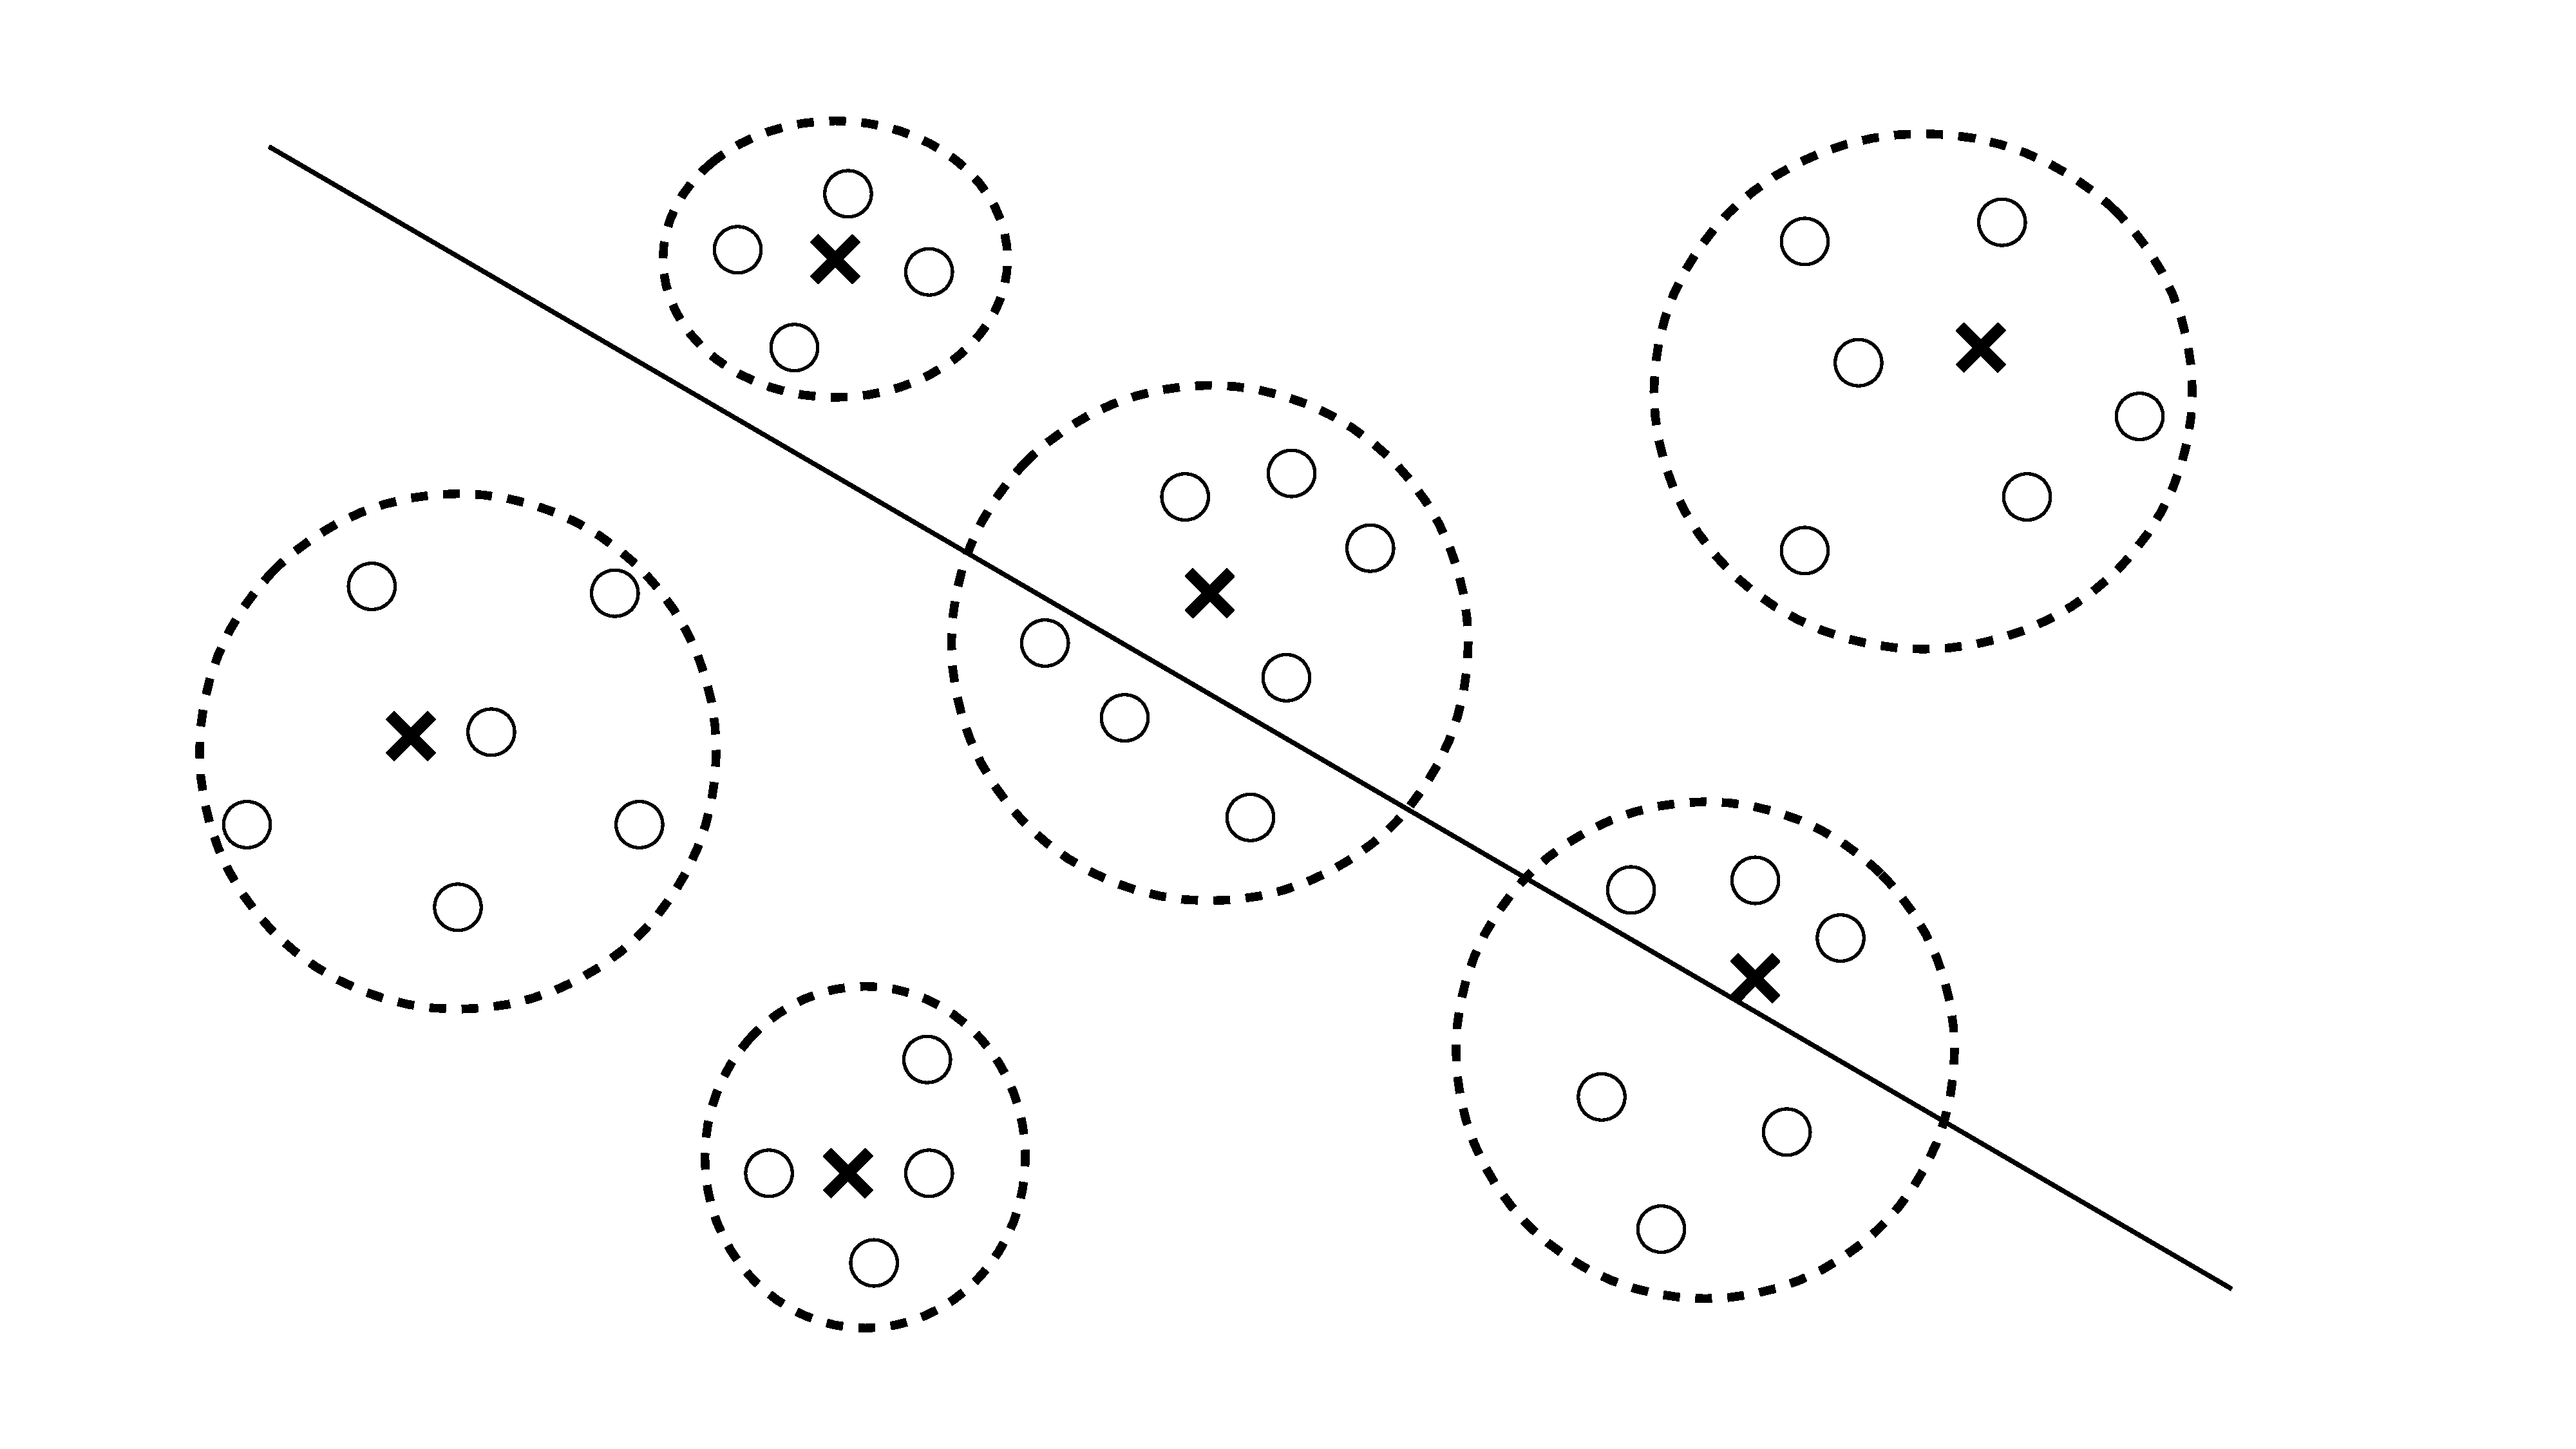
\includegraphics[width=6cm]{pics/chapter2/aid-demo-a.pdf}
    \captionof{figure}{}
    \end{subfigure}
    \begin{subfigure}[t]{0.3\textwidth}\label{aid-demo2}
    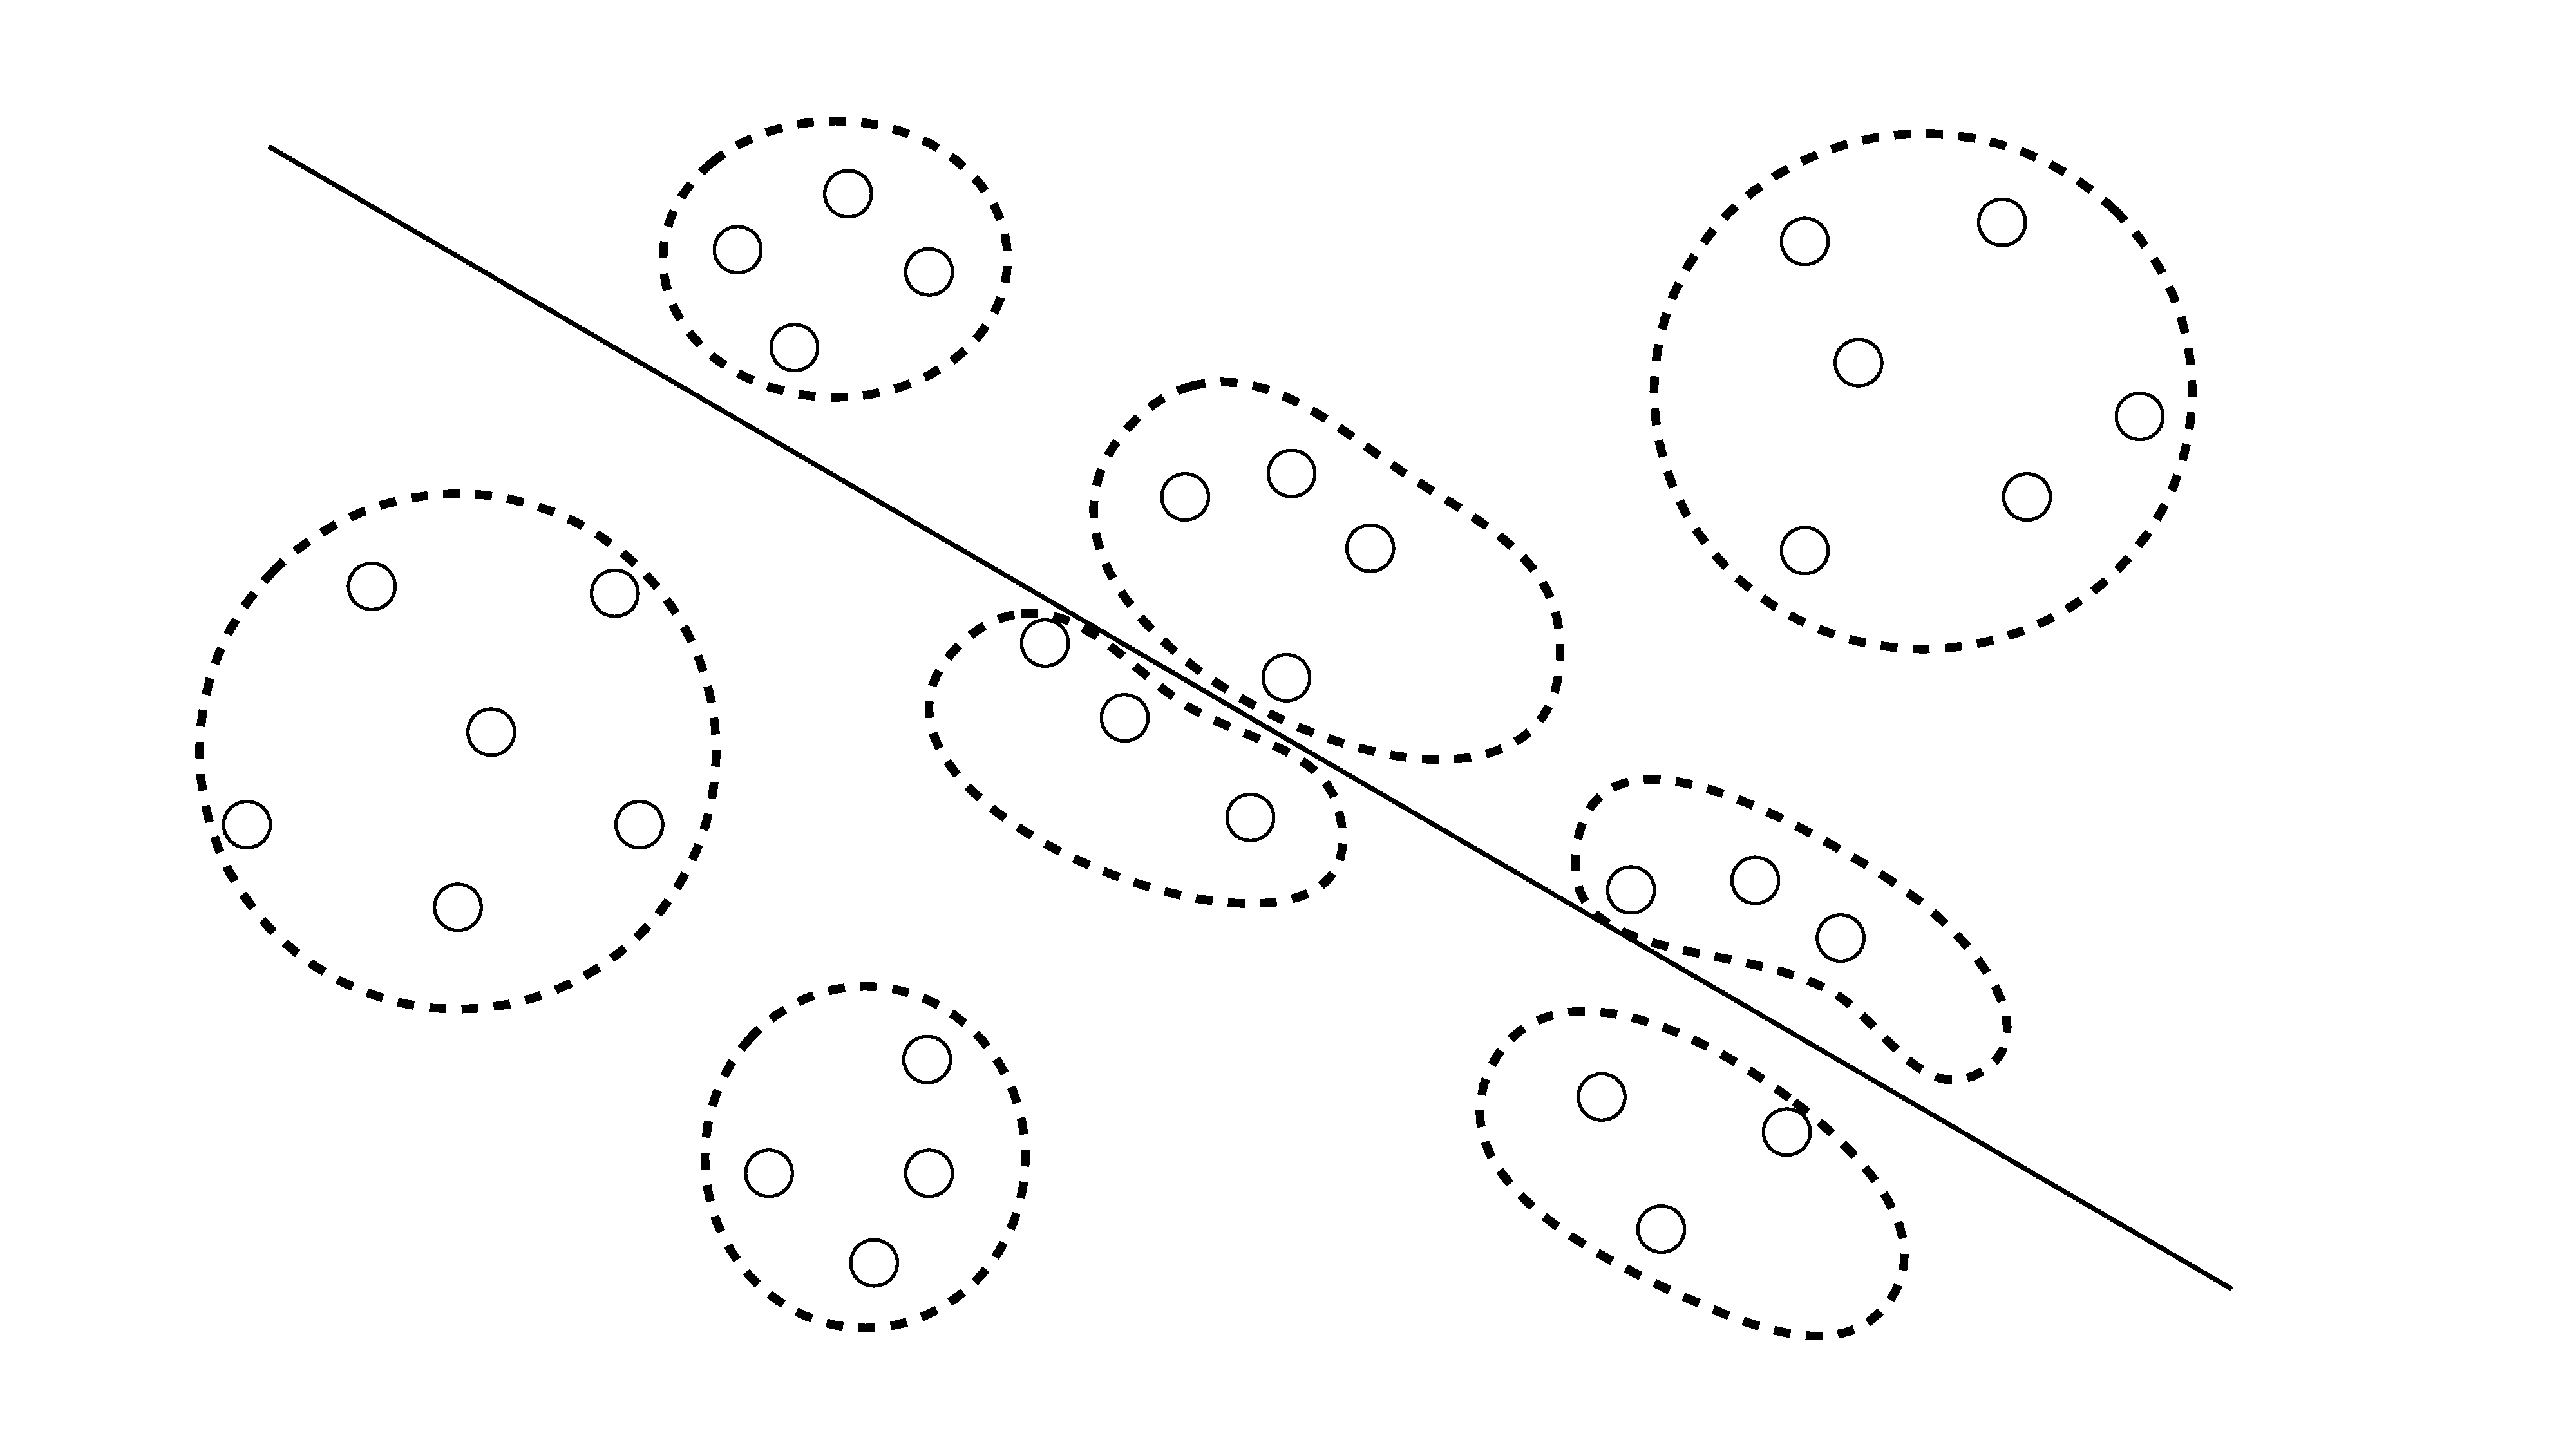
\includegraphics[width=6cm]{pics/chapter2/aid-demo-b.pdf}
    \captionof{figure}{}
    \end{subfigure}
    \begin{subfigure}[t]{0.3\textwidth}\label{aid-demo3}
    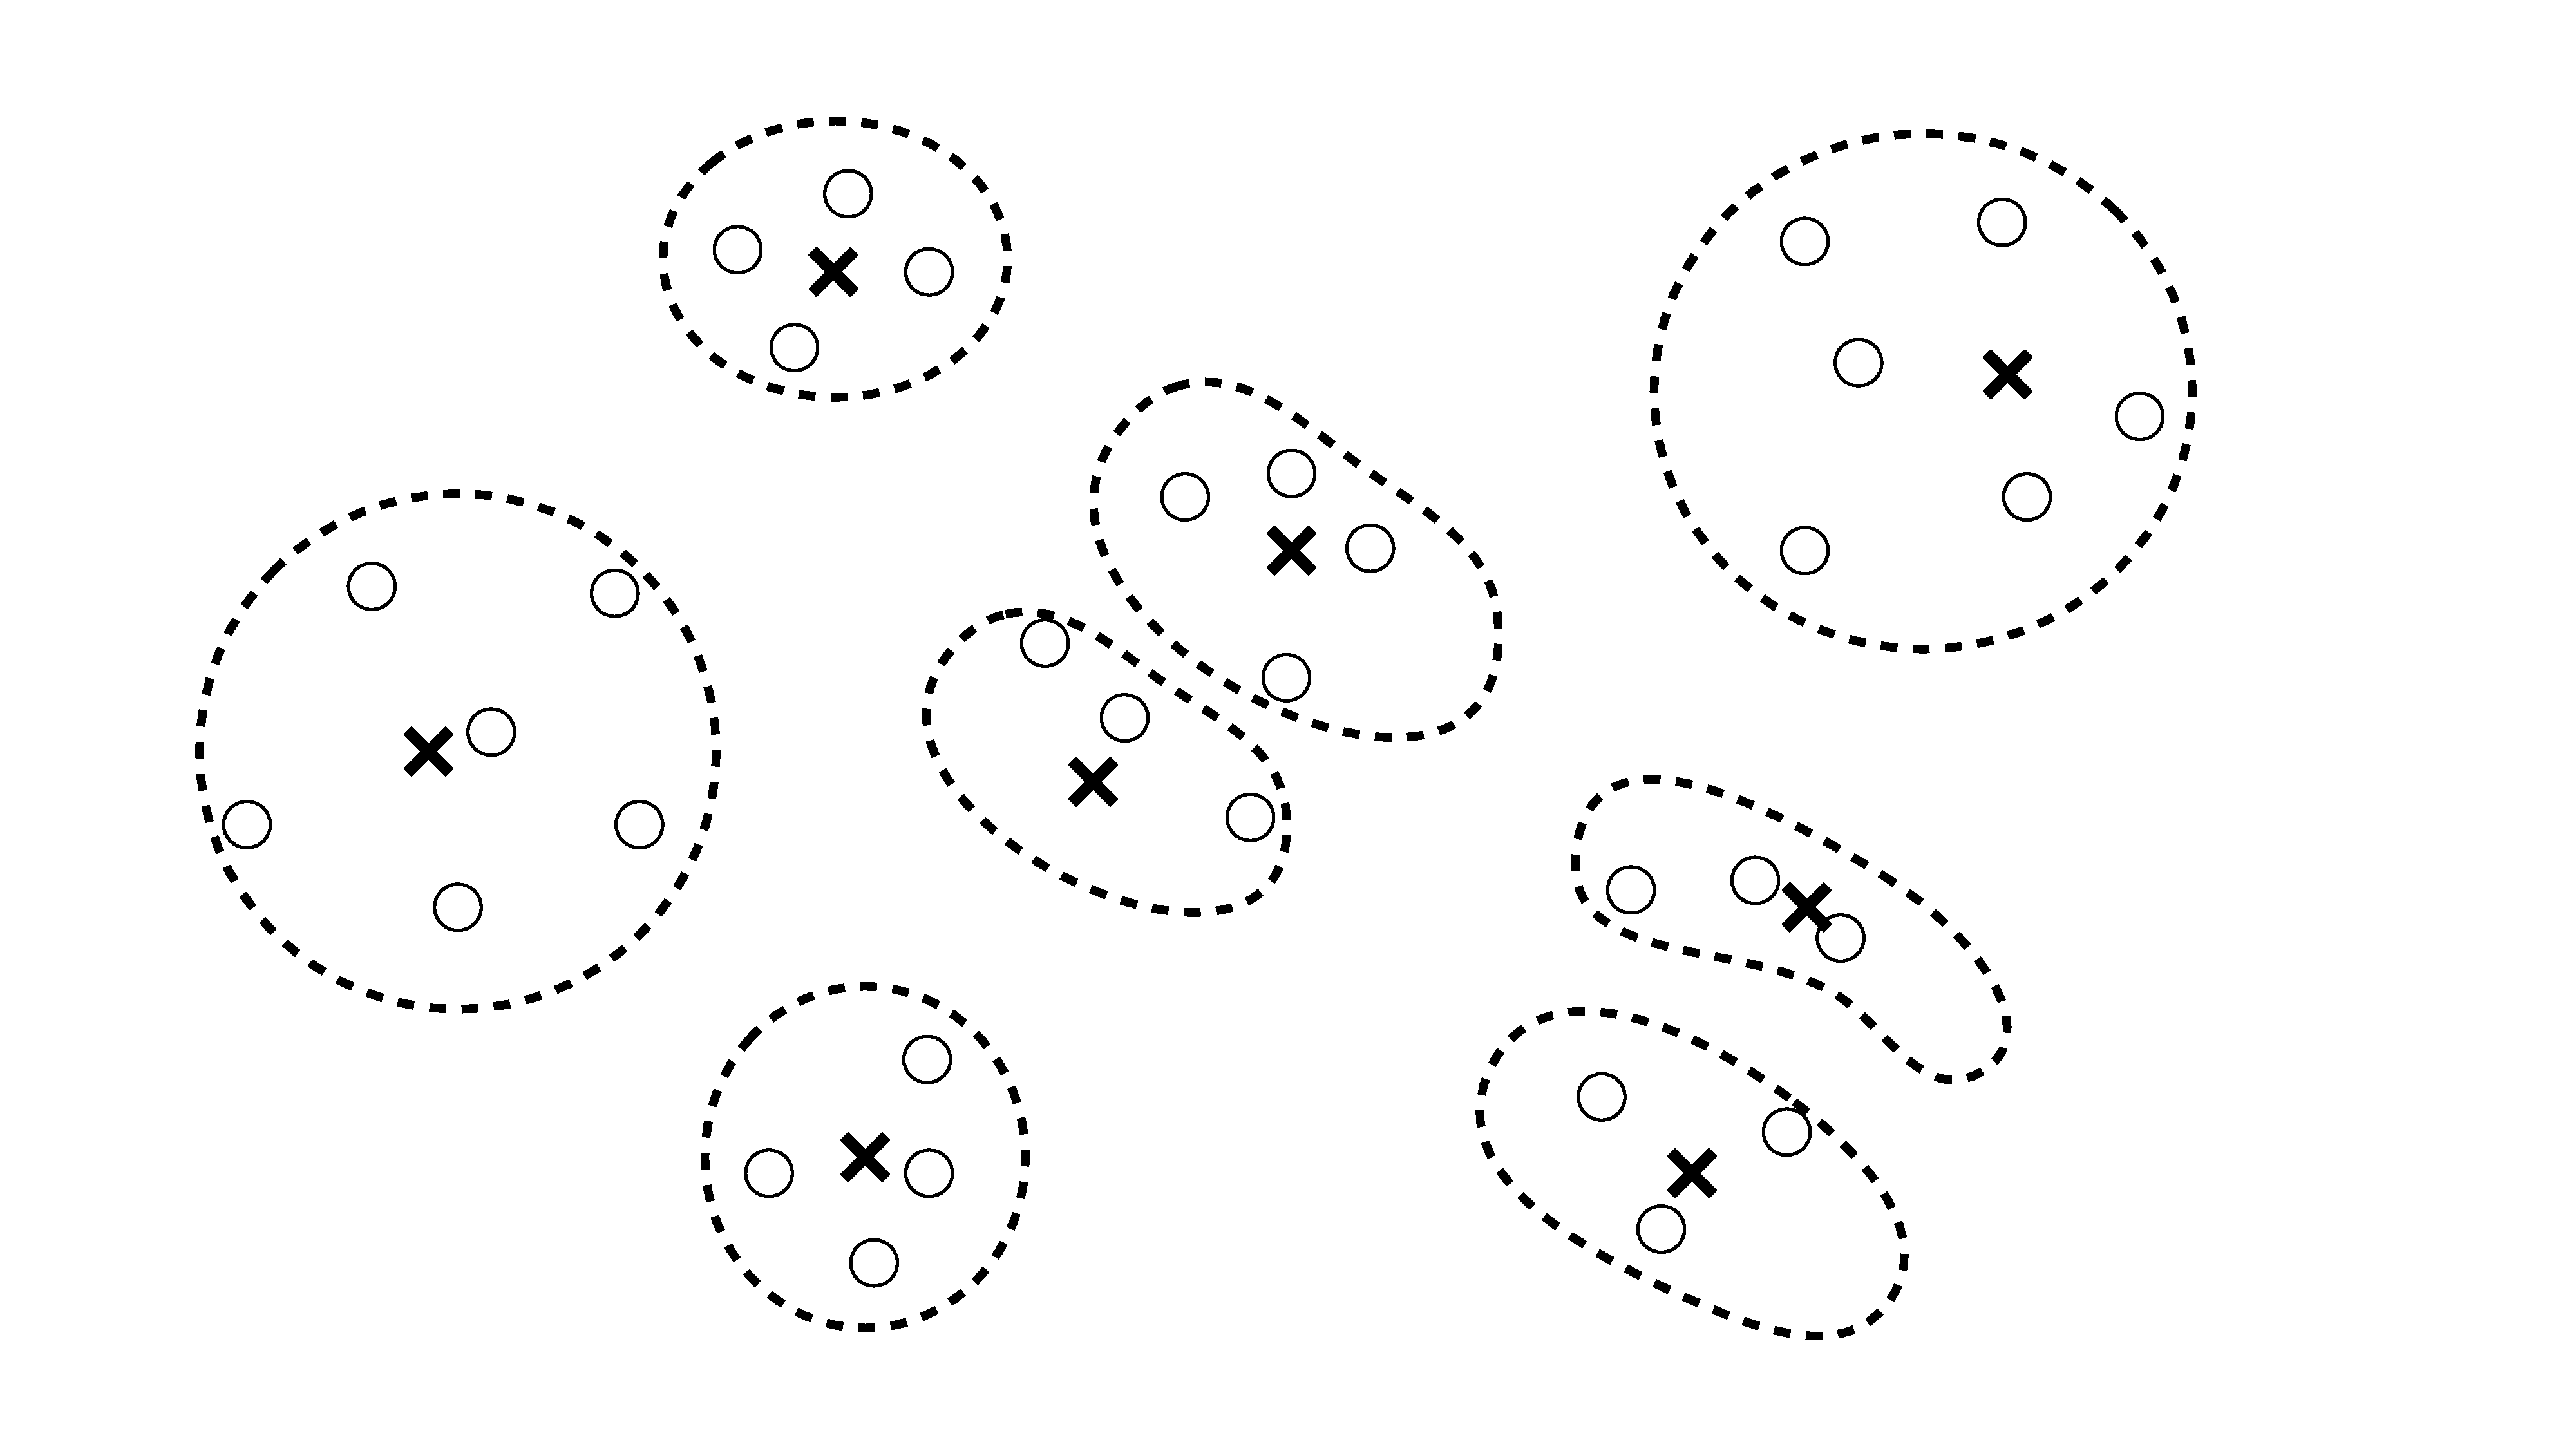
\includegraphics[width=6cm]{pics/chapter2/aid-demo-c.pdf}
    \captionof{figure}{}
    \end{subfigure}
    \caption{\small 聚类拆解步骤示意图}
    \label{aid-demo}

\end{figure}

结合算法3.1,到这里已经给出了完成聚类——迭代拆解最小绝对值回归的所有计算步骤,当聚类无法继续划分时,迭代终止。

下面证明最后一次迭代的解$\hat{\bm{\beta}}^{(\tau)}$就是\eqref{l1loss2}的解$\bm{\beta}^*$,
\begin{equation*}
    \begin{split}
        \xi^* & = \sum_{i \in I} |y_i - \sum_{j \in J}x_{ij}\bm{\beta}_j^*|
        = \sum_{k \in K^{(t)}}\sum_{i \in C_k^{(t)}}|y_i - \sum_{j \in J}x_{ij}\bm{\beta}_j^*| \\
        & \geq \sum_{k \in K^{(t)}}|\sum_{i\in C_k^{(t)}}(y_i - \sum_{j \in J}x_{ij}\bm{\beta}_j^*)|
        = \sum_{k \in K^{(t)}}|C_k^{(t)}||y_k^{(t)} - \sum_{j \in J}x_{kj}^{(t)}\bm{\beta}_j^*|\\
        & \geq \sum_{k \in K^{(t)}} |C_k^{(t)}||y_K^{(t)} - \sum_{j\in J}x_{kj}^{(t)} \hat{\bm{\beta}}_j^{(t)}|
        = \sum_{k \in K^{(t)}} |\sum_{i \in C_k^{(t)}} y_i - \sum_{i \in C_k^{(t)}}\sum_{j \in J}x_{ij}\hat{\bm{\beta}}_j^{(t)}| \\
        & = \sum_{k \in K^{(t)}} \sum_{i \in C_k^{(t)}}|y_i - \sum_{j \in J}x_{ij}\hat{\bm{\beta}}_j^{(t)}|
        = \sum_{i \in I}|y_i - \sum_{j \in J} x_{ij} \hat{\bm{\beta}}_j^{(t)}| 
        = \xi^{(t)}
    \end{split}
\end{equation*}

因为$\hat{\bm{\beta}}_j^{(t)}$是\eqref{l1loss2}的可行解,又显然$\xi^* \leq \xi^{(t)}$,
这就证明了$\xi^* = \xi^{(t)}$,注意到$ \sum_{k \in K^{(t)}} |C_k^{(t)}||y_K^{(t)} - \sum_{j\in J}x_{kj} \hat{\bm{\beta}}_j^{(t)}|$
就是$F^{(t)}$,因此$\xi^{(t)} = F^{(t)}$。因此最后一次迭代$F^{(\tau)}$的最优解$\hat{\bm{\beta}}^{(\tau)}$就是原问题的最优解。

\subsubsection{优化带有惩罚项的最小绝对值回归}
前面给出的算法已经在很大程度上优化了在处理高维宏观经济变量时,最小绝对值回归计算性能的问题。
而在高维宏观经济实证研究中,变量的维数众多,在建立最小绝对值回归模型时,还需要考虑到变量筛选问题。

对于\eqref{l1losstotal},为了进行变量的筛选,我们需要对估计量$\bm{\beta}^*$的维数做出约束,
一般来说,我们通常采用以下3三种方法:1)$\|\bm{\beta}\|_0 = p$,可以直接选择入选变量的个数;
2)$\|\bm{\beta}\|_2 < s$,该法又称为岭回归;3)$\|\bm{\beta}\|_1 < s$,即为常用的$L_1$正则化方法。
通过加入新的约束,问题的形式也发生了变化。

Park等人于2019年的研究中给出了进一步的结论,对于问题
\begin{equation}\label{l1conclusion}
    E^* = \underset{B\in \phi}{\operatorname{min}} ||Y - f(X, B)||_{L_1}
\end{equation}
其中$Y$为模型响应变量数据矩阵,$X$为解释变量数据矩阵,$B$为模型系数矩阵,$\phi$为模型系数的约束条件。
$f$为任一目标函数,若$f$满足条件
\begin{equation}\label{fcondition}
    f(B, WX) = Wf(B, X)
\end{equation}
其中$W$为一权重矩阵。那么就可以通过聚类——迭代拆解算法求原优化问题的最优解。

而在岭回归和LASSO中,都通过给目标函数加上惩罚项来进行求解,岭回归对应的惩罚项$s\sum_{i=1}^p\bm{\beta}_i^2$,
$L_1$正则化对应的惩罚项为$s\sum_{i=1}^p|\bm{\beta}_i|$,容易发现,加入惩罚项后目标函数仍然满足\eqref{fcondition}
。因此,对于需要进行变量筛选的高维最小绝对值回归问题,我们可以修改目标函数,通过算法3.1解决。
对于携带正则项的最小绝对值回归,也可以通过线性规划来处理\cite{wang2006regularized}。

\subsection{一种基于替代变量的估计方法}
聚类——迭代拆解算法是通过有效减少$L_1$目标函数最小化的问题规模来提升求解性能,
每一次迭代仍需要通过线性规划方法求解$L_1$目标函数的最小化问题。
Weidong Liu等人于2020年提出了一种基于替代变量的估计方法\cite{svn},通过替代变量将分位数损失函数转化为$L_2$损失函数,
避免使用线性规划求解分位数损失,因此可以显著提升一般分位数回归的求解性能。

考虑到最小绝对值回归为其特殊情形,因此该算法可以在一定程度上解决最小绝对值回归的性能问题。
下面我们介绍如何将该方法应用在最小绝对值回归的场景下,并且给出具体的计算步骤。

\subsubsection{基于替代变量的迭代算法}
考虑\eqref{l1losstotal},
对目标函数稍作形式变换,其中$\rho(x) = x(0.5 - \mathbb{I}[x \leq 0])$,
$\mathbb{I}(x)$为指示函数。
\begin{equation}
\bm{\beta}^* = \underset{\bm{\beta} \in \mathbb{R}^{p}}{\operatorname{arg\ min}}\mathbb{E}|Y - \bm{X}^T\bm{\beta}| = 
\underset{\bm{\beta} \in \mathbb{R}^{p}}{\operatorname{arg\ min}}\mathbb{E}\rho(Y - \bm{X}^T\bm{\beta})
\end{equation}
若已知n\ $i.i.d.$ 的样本$(\bm{X}_i, Y_i)\ (1 \leq i \leq n)$,令$\hat{\bm{\beta}}$为$\bm{\beta}^*$的估计量,
\begin{equation}\label{rho-problem}
    \hat{\bm{\beta}} = \underset{\bm{\beta} \in \mathbb{R}^{p}}{\operatorname{arg\ min}}\frac1{n}\sum_{i=1}^{n}\rho(Y_i - \bm{X}_i^T\bm{\beta}).
\end{equation}

一般地,我们使用牛顿迭代法求解某随机优化问题:
\begin{equation}\label{randomversion}
    \bm{\beta}^* = \underset{\bm{\beta} \in \mathbb{R}^{p}}{\operatorname{arg\ min}} \mathbb{E}[G(\bm{\beta};\bm{X},Y)]
\end{equation}
其中$G(\bm{\beta};\bm{X}, Y)$是损失函数,$\bm{X}$和$Y$分别是$p$维自变量和一元响应变量,$\bm{\beta}$为回归系数。使用牛顿-拉弗森迭代来求解,
\begin{equation}
    \tilde{\bm{\beta}}_1 = \bm{\beta}_0 - \bm{H}(\bm{\beta}_0)^{-1}\mathbb{E}[g(\bm{\beta};\bm{X},Y)]
\end{equation}
其中$\bm{\beta}_0$是一个初始估计,$g(\bm{\beta};\bm{X},Y)$为损失函数$G(\bm{\beta};\bm{X},Y)$关于$\bm{\beta}$的梯度。\\
$\bm{H}(\bm{\beta}):=\partial\mathbb{E}[g(\bm{\beta};\bm{X},Y)
/\partial\bm{\beta}$表示$\mathbb{E}G(\bm{\beta};\bm{X},Y)$的海森矩阵(Hessian Matrix)。特别地,我们这里考虑损失函数为$L_1$损失的特殊情形,
\begin{equation}\label{rho-condition}
    G(\bm{\beta};\bm{X},Y) = \rho(Y - \bm{X}^T\bm{\beta})
\end{equation}
在\eqref{rho-condition}的情形下,$g(\bm{\beta};\bm{X},Y) = \bm{X}(\mathbb{I}[Y - \bm{X}^T\bm{\beta} < 0] - 0.5)$。

并且$\bm{H}(\bm{\beta}) = \mathbb{E}(\bm{X}\bm{X}^Tf(\bm{X}^T(\bm{\beta} - \bm{\beta}^*)))$,这里
$f(x)$是噪声$e$的密度函数。当初始估计量$\bm{\beta}_0$和$\bm{\beta}^*$很接近时,$\bm{H}(\bm{\beta}_0)$就会很接近
$\bm{H}(\bm{\beta}^*) = \bm{\Sigma}f(0)$,这里$\bm{\Sigma} = \mathbb{E}\bm{X}\bm{X}^T$是$\bm{X}$的协方差
矩阵。使用$\bm{H}(\bm{\beta}^*)$替换$\bm{H}(\bm{\beta}_0)$,可得

\begin{equation}\label{rho-beta1}
    \bm{\beta}_1 = \bm{\beta}_0 - \bm{H}(\bm{\beta}^*)^{-1}\mathbb{E}[g(\bm{\beta};\bm{X}, Y)]
    = \bm{\beta}_0 - \bm{\Sigma}^{-1}f^{-1}(0)\mathbb{E}[g(\bm{\beta}_0;\bm{X},Y)]
\end{equation}
在$\bm{\beta}^*$处对$\mathbb{E}[g(\bm{\beta}_0;\bm{X},Y)$进行泰勒展开,
\begin{equation*}
    \begin{split}
\mathbb{E}[g(\bm{\beta}_0;\bm{X},Y) &= \bm{H}(\bm{\beta}^*)(\bm{\beta}_0 - \bm{\beta}^*) + O(|\bm{\beta}_0 - \bm{\beta}^*|_2^2) \\
 &= \bm{\Sigma}f(0)(\bm{\beta}_0 - \bm{\beta}^*) + O(|\bm{\beta}_0 - \bm{\beta}^*|_2^2)
    \end{split}
\end{equation*}
结合\eqref{rho-beta1},可以得到
\begin{equation*}
    \begin{split}
        |\bm{\beta}_1 - \bm{\beta}^*|_2 &=  |\bm{\beta}_0 - \bm{\Sigma}^{-1}f^{-1}(0)(
            \bm{\Sigma}f(0)(\bm{\beta}_0 - \bm{\beta}^*) + O(|\bm{\beta}_0 - \bm{\beta}^*|_2^2)
        ) - \bm{\beta}^*|_2\\
        &= O(|\bm{\beta}_0 - \bm{\beta}^*|_2^2)
    \end{split}
\end{equation*}
因此,如果我们得到一个$\bm{\beta}^*$的一致估计量$\bm{\beta}_0$,我们就可以通过\eqref{rho-beta1}得到
偏误更小的估计。

下面我们将\eqref{rho-beta1}转化成一个最小二乘问题。首先我们重写该式,
\begin{equation}
    \begin{split}
    \bm{\beta}_1 &= \bm{\Sigma}^{-1}(\bm{\Sigma}\bm{\beta}_0 - f^{-1}(0)\mathbb{E}[g(\bm{\beta}_0;\bm{X},Y)])\\
    &= \bm{\Sigma}^{-1}\mathbb{E}[\bm{X}\{\bm{X}^T\bm{\beta}_0 - f^{-1}(0)(\mathbb{I}[Y \leq \bm{X}^T\bm{\beta}_0] - 0.5)\}]
    \end{split}
\end{equation}
这里我们定义一个新的响应变量$\tilde Y$,
\begin{equation}
    \tilde Y = \bm{X}^T\bm{\beta}_0 - f^{-1}(0) (\mathbb{I}[Y \leq \bm{X}^T\bm{\beta}_0] - 0.5)
\end{equation}
那么$\bm{\beta}_1 = \bm{\Sigma}^{-1}\mathbb{E}(\bm{X}\tilde{Y})$就是线性回归问题$\tilde Y = \bm{X}^T\bm{\beta}$
的最优回归系数,即
\begin{equation}\label{beta1-original}
    \bm{\beta}_1 = \underset{\bm{\beta} \in \mathbb{R}^{p}}{\operatorname{arg\ min}} 
    \mathbb{E}(\tilde Y - \bm{X}^T \bm{\beta})^2
\end{equation}
给定$i.i.d.$样本$(\bm{X}_i, Y_i)$,构造
\begin{equation}\label{svny}
    \tilde{Y}_i = \bm{X}_i^T\hat{\bm{\beta}}_0 - \hat{f}^{-1}(0)
    (\mathbb{I}[Y_i \leq \bm{X}_i^T \hat{\bm{\beta}}_0] - 0.5)
\end{equation}
其中$\hat{\bm{\beta}}_0$为$\bm{\beta}^*$的一个初始估计,$\hat{f}(0)$为$f(0)$的一个估计
\begin{equation}\label{yl2loss}
    \hat{\bm{\beta}} = \underset{\bm{\beta} \in \mathbb{R}^{p}}{\operatorname{arg\ min}}
    \frac1{n} \sum_{i=1}^n(\tilde{Y}_i - \bm{X}_i^T\bm{\beta})^2
\end{equation}
这里我们选择某估计量作为$\hat{\bm{\beta}}_0$,并且采用$f(0)$的核密度估计作为$\hat{f}(0)$,

$$
    \hat{f}(0) = \frac1{nh}\sum_{i=1}^nK(\frac{Y_i - \bm{X}^T_i\hat{\bm{\beta}}_0}{h})
$$
其中$K(x)$为核函数,$h \rightarrow 0$是带宽,本方法
在每次迭代都需要调整带宽\cite{svn}。

只要给定的初始值$\hat{\bm{\beta}}_0$是$\bm{\beta}^*$的一致估计量,那么$\hat{\bm{\beta}}$就将会是一个更加接近
$\bm{\beta}^*$的新的估计,并且\eqref{yl2loss}为最小二乘问题,其计算十分简便。

我们当然可以将$\hat{\bm{\beta}}$作为\eqref{rho-beta1}的初始值,这样继续构造替代变量进行迭代,最终收敛到$\bm{\beta}^*$。
算法3.2给出了使用替代变量估计方法的计算步骤。
\begin{table}[H]%%%%%%开始表格
    \centering%把表居中
    \begin{tabular}{{p{0.9\columnwidth}}}%三个c代表该表一共三列,内容全部居中
    
    \toprule%第一道横线 表头
    {\heiti 算法}{\bf 3.2} 使用替代变量迭代算法方法求解最小绝对值回归问题(SVN, Substitue Variable Newton method)\\
    \midrule%第二道横线 符号+解释+单位 中间用&隔开
    输入:$Y$和$\bm{X}$的样本$\bm{Y} = (Y_1, Y_2, ..., Y_n)$,$\bm{X} = (\bm{X}^{\rm T}_1, \bm{X}^T_2, ..., \bm{X}^T_n)$,
    迭代次数$\tau$,核函数$K(x)$,依赖于迭代次数的带宽$h^{(t)}$,$(t = 1, ..., \tau)$。
    \\
    初始化:给出初始相合估计量$\hat{\bm{\beta}}^{0} $,将样本划分成$J$个均等子集,样本量均为$m$,为了给出最小绝对值回归估计量的相合估计,
    我们取任一子集里面的数据,直接使用最小一乘法估计$\hat{\bm{\beta}}^{0}$。
    \\
    对于$t = 1, ..., \tau$:
    取新的数据子集,在该数据集上
    \\
        1. 计算$\hat{f}^{(t)}(0)$,
        $$
        \hat{f}^{(t)}(0) = \frac1{mh}\sum_{i=1}^{m}K(\frac{Y_i - \bm{X}_i^T\hat{\bm{\beta}}^{(t-1)}}{h^{(t)}})
        $$
    \\
        2. 计算$\tilde{Y} = (\tilde Y_1, \tilde Y_2, ..., \tilde Y_m)$,
        $$
        \tilde{Y}_i = \bm{X}^T_i\hat{\bm{\beta}}^{(t-1)} - \hat{f}^{(t)}(0)^{-1}
        (\mathbb{I}[Y_i \leq \bm{X}_i^T \hat{\bm{\beta}}^{(t-1)}] - 0.5)
        $$
    \\
        3. 计算$\hat{\bm{\beta}}^{(t)}$,
        $$
        \hat{\bm{\beta}}^{(t)} = \underset{\bm{\beta} \in \mathbb{R}^{p}}{\operatorname{art\ min}}
        \frac1{m}\sum_{i=1}^m (\tilde{Y}_i - \bm{X}_i^T\bm{\beta})^2
        $$
    \\
    输出:$\hat{\bm{\beta}}^{(\tau)}$
    \\
    \bottomrule%第三道横线
    \end{tabular}
\end{table}%%%%%%结束表格

\subsubsection{优化带有惩罚项的最小绝对值回归}
在高维相依自变量的情形下,我们只需在\eqref{beta1-original}加入惩罚项即可,例如我们使用$L_1$正则化,那么
\begin{equation}
    \bm{\beta}_{1, \lambda} =\underset{\bm{\beta} \in \mathbb{R}^{p}}{\operatorname{arg\ min}} 
    \mathbb{E}(\tilde Y - \bm{X}^T \bm{\beta})^2 + \lambda|\bm{\beta}|
\end{equation}
对应的,最终估计量计算如下
\begin{equation}\label{beta1-lasso}
    \hat{\bm{\beta}} = \underset{\bm{\beta} \in \mathbb{R}^{p}}{\operatorname{arg\ min}}
    \frac1{n} \sum_{i=1}^n(\tilde{Y}_i - \bm{X}_i^T\bm{\beta})^2 + \lambda|\bm{\beta}|
\end{equation}
\eqref{beta1-lasso}是著名的LASSO问题,已经有了快速解决的算法。因此对于高维情形算法3.2仅需稍作改动,
直接更换目标函数即可。

\subsection{模拟实验}
本章前面两节介绍了聚类——迭代拆解算法和一种基于替代变量的迭代算法,
前者通过减小问题规模、逐步逼近最优解的方法来提升计算性能,
而后者通过变量替换的方法将最小绝对值回归问题转化为最小二乘问题,在给定一个相合估计条件下逼近最优解。
两种方法都可以处理带有惩罚项和不带有惩罚项的最小绝对值回归问题,并且前文已经给出了两种算法实现的具体步骤。

本节将通过一个数值模拟实验来比较和分析两种方法的性能表现,分析算法的收敛情况,
并对算法的解的确性进行观察。

\subsubsection{数据准备}
为测试两种算法求解一般最小绝对值回归问题的性能,设定模拟数据来自下面的模型:
\begin{equation*}
    {Y}_i = \bm{X}_i^T \bm{\beta} + e_i, i = 1, 2, ..., n.
\end{equation*}
其中$\bm{X}_i = (1, X_{i,1}, ..., X_{i, p-1})$为$p$维随机向量。
假设$\bm{X}$的各维独立并服从正态同分布,$\bm{e}$为高斯噪声。
我们设置不同$p, n$的组合用来测试算法的计算性能,并观察在不同的噪声分布下,估计结果的准确性。
对于系数$\bm{\beta}$,设$l$为其$L_0$范数,取
$$
    \bm{\beta} = (\frac{10}{l}, \frac{20}{l}, ..., \frac{10(l-1)}{l}, 10, 0, ..., 0).
$$

算法2.1(以下简称SVN)的每步最佳带宽依赖于数据集的性质,参考Weidong Liu等\cite{svn},这里给出
$$
    h^{(t)} = \sqrt{\frac{s\log n}{n}} + s^{-1/2} (\frac{s^2\log n}{10m})^{(t+1)/2},
$$
其中$m$为每个子样本的大小,核函数选取高斯核函数,其中$s$的理论最优取值和$l$有关,而本次实验中取常数。

对于聚类——迭代拆解算法,我们这里选择初始聚类方法如下:
首先从原始数据中少量采样(本实验取$max\{0.5\%n, p\}$),通过最小绝对值回归给出系数估计$\bm{\beta}^{init}$,
对每一个原始数据点,计算其在当前模型系数下的残差,然后进行K-means聚类得到$C^0$。

本次实验最小绝对值回归性能测试的对比基准方法是:线性规划内点法(以下简称LP);

我们给出了SVN算法和AID算法的Python3实现,数值计算基于Numpy包,
作为基准的LP使用Scipy数值计算包的对应实现。

\subsubsection{实验结果}
我们采用最终估计值和真实值差的$L_2$范数来衡量准确性。
在实验结果中中我们着重观察算法的收敛性、算法的准确性和计算性能。

首先我们在最小绝对值回归模型下,比较三种算法的性能表现。
表\ref{tab-performance}中,$r^0$表示AID算法初始聚类$K_0/n$的值,而$r^\tau$表示算法终止时$K_\tau/n$的取值。
需要注意的是,对于AID算法,$\tau$表示算法终止时经历的迭代次数,Time表示算法终止时运算的cpu时间。
而对于SVN算法,$\tau$表示在当前带宽选择下使其每估计值达到稳定的迭代次数,Time表示全部数据参与迭代完毕经历的cpu时间
(处理机情况:苹果M1芯片8核,8GB内存,OSX,CPython解释器3.82Arm版)。
\begin{table}[H]
    \small
    \caption{\small 高斯噪声下三种估计算法的性能比较}
    \label{tab-performance}
    \centering
    \begin{tabular}{@{}ccccccccc@{}}
    \toprule
           &     & \multicolumn{4}{c}{AID}        & \multicolumn{2}{c}{SVN} & LP        \\ \midrule
    n      & p   & $r^0$(\%) & $r^\tau$(\%) & $\tau$  & Time(sec) & $\tau$      & Time(sec)      & Time(sec) \\ \midrule
    20000  & 10  & 0.05  & 2.90  & 6  & 2         &  3      &         0.38       & 0.20      \\
    20000  & 50 & 0.15  & 12.00 & 12 & 13        &   7     &          6     & 3       \\
    20000  & 100 & 0.15  & 12.00 & 12 & 38        &  11      &         27    & 21         \\
    20000  & 200 & 0.66  & 21.55 & 9  & 118        &   8     &          76      & 126        \\
    20000  & 500 & 0.80  & 28.00 & 11 &  535      &  3      &              322  &     813 \\ 
    40000  & 10  & 0.05  & 2.90  & 6  & 3        &  3      &         0.74      & 0.23     \\
    40000  & 50 & 0.15  & 12.00 & 12 & 31        &   7     &          14     & 7       \\
    40000  & 100 & 0.15  & 12.00 & 12 & 84       &  8      &         56    & 48         \\
    40000  & 200 & 0.66  & 21.55 & 9  & 210        &   8     &          154     & 258        \\
    40000  & 500 & 0.80  & 28.00 & 11 & 1965       &  3      &             1143   &  3446      \\ 
    200000  & 100 & 0.80  & 11.00 & 11 & 134       &  3      &          361      &   496     \\ 
    200000  & 200 & 0.80  & 28.00 & 11 & 2476       &  3      &          1631      &   3329     \\ 
    \bottomrule
    \end{tabular}
\end{table}

从表\ref{tab-performance}可以看出在$n,p$较大场合下,AID算法和SVN算法均在性能上领先,尤其是SVN算法具有更好的性能表现,
因为以上时间为训练全部数据需要的时间,而在下面可以看到SVN算法具有相当快的收敛速度,在后续性能比较中,我们会
将SVN算法的停止条件设定为相邻两次迭代的$\hat{\bm{\beta}}^t$夹角小于某个的小正数,能够进一步缩短SVN算法的时间。

接下来我们观察不同噪声分布对估计准确性的影响,这里主要观察SVN算法的准确性(注意AID算法的解就是LP最优解,
因此它的准确性是不言自明的)。
图\ref{svn-noise}显示了不同的噪声分布下SVN算法的表现,其中横轴代表迭代的次数,其中$n=20000,p=50,s=20$,
图(a)、(b)、(c)分别为高斯噪声、指数噪声和柯西噪声。
可以看到,随着迭代进行,SVN算法估计值随样本信息不断调整,始终保持在和LP解相差不大的水平上
;SVN算法仅在柯西噪声这种极端重尾场景下,表现稍差。

\begin{figure}[H]
    \centering
    \begin{subfigure}[t]{0.3\textwidth}\label{svn-demo1}
    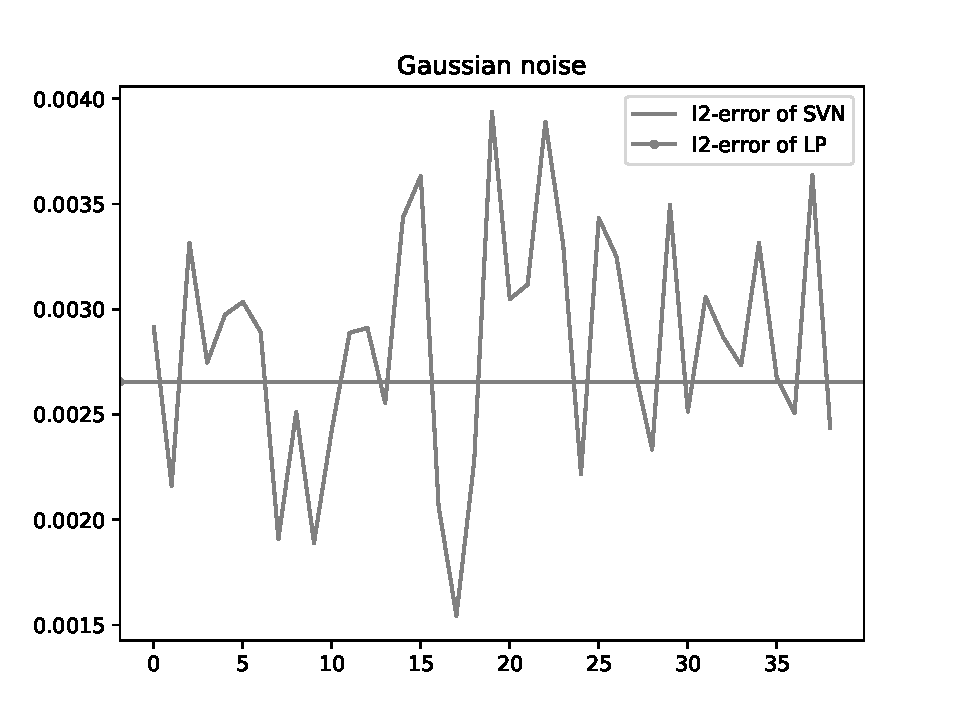
\includegraphics[width=5.5cm]{pics/chapter2/gaussian-svn.pdf}
    \captionof{figure}{}
    \end{subfigure}
    \begin{subfigure}[t]{0.3\textwidth}\label{svn-demo2}
    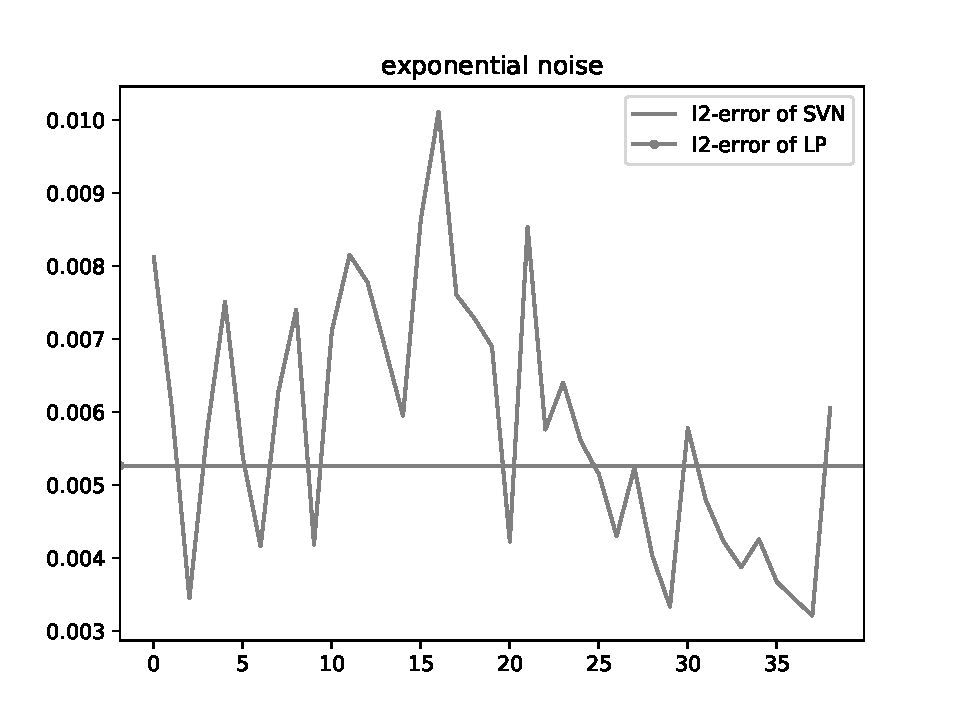
\includegraphics[width=5.5cm]{pics/chapter2/exp-svn.pdf}
    \captionof{figure}{}
    \end{subfigure}
    \begin{subfigure}[t]{0.3\textwidth}\label{svn-demo3}
    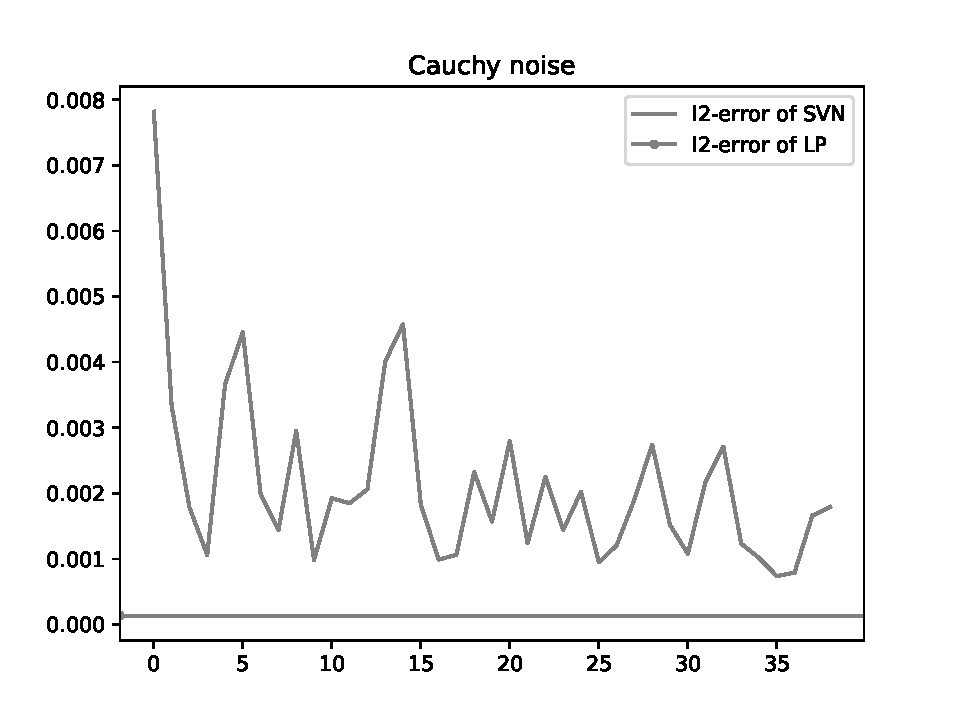
\includegraphics[width=5.5cm]{pics/chapter2/cauchy-svn.pdf}
    \captionof{figure}{}
    \end{subfigure}
    \caption{ \small SVN算法在各种噪声下的表现}
    \label{svn-noise}
\end{figure}

主要到算法3.2中我们使用最小绝对值回归估计量作为初始估计。在柯西噪声下,我们考虑了
最小二乘估计量作为初始估计的情况,来观察SVN算法的准确性。

\begin{figure}[H]
    \centering
    \begin{subfigure}[t]{0.3\textwidth}\label{svn-demo2}
    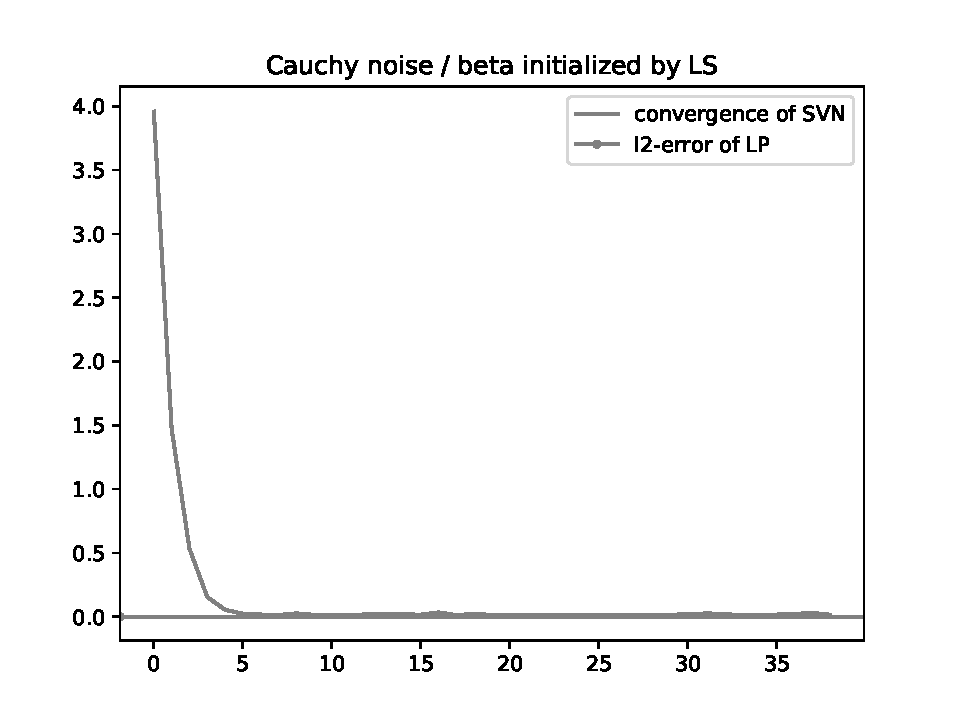
\includegraphics[width=5.5cm]{pics/chapter2/l2-svn-demo.pdf}
    \captionof{figure}{}
    \end{subfigure}
    \begin{subfigure}[t]{0.3\textwidth}\label{svn-demo3}
    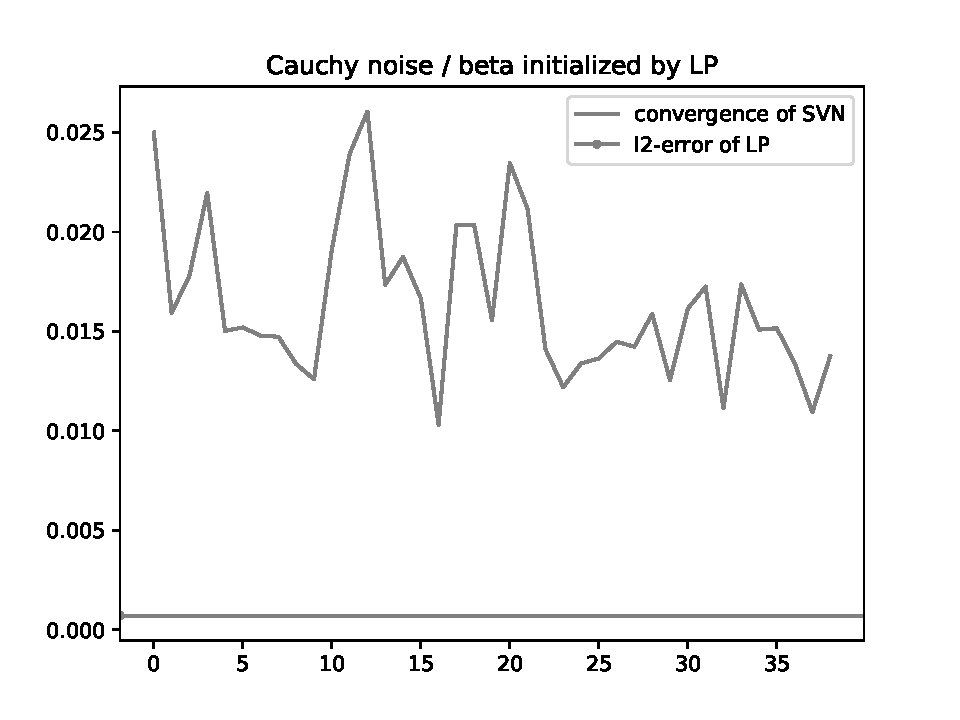
\includegraphics[width=5.5cm]{pics/chapter2/l1-svn-demo.pdf}
    \captionof{figure}{}
    \end{subfigure}
    \caption{ \small 最小二乘估计初始化}
    \label{svn-l2-demo}
\end{figure}

图\ref{svn-l2-demo}中横轴代表示迭代次数,纵轴代表示估计的误差平方和。实验结果表明,
选择最小二乘估计量作为初始值,SVN算法依然能够很快收敛。这启发我们
在使用最小绝对值回归时,如果最小二乘估计量是相合的,那么也可以通过最小二乘估计量产生初始估计,
这样一来,在计算中可做到完全避免直接求解最小绝对值回归问题。

需要说明的是,SVN算法的收敛速度和带宽选择有很大关系。
在选择了足够小的带宽时,SVN算法可快速收敛。图\ref{svn-demo}展示了SVN算法的收敛情况,
其中横轴代表示迭代次数,纵轴代表示相邻两次$\bm{\beta}$估计之差的平方和。
观察到SVN算法在带宽较小时收敛速度表现较好,这也符合该算法提出的理论基础。
在带宽选择较小($s$较小)时,SVN算法能够迅速收敛。
当然,如果我们选择了很大的带宽那么算法不能收敛。
\begin{figure}[H]
    \centering
    \begin{subfigure}[t]{0.3\textwidth}\label{svn-demo1}
    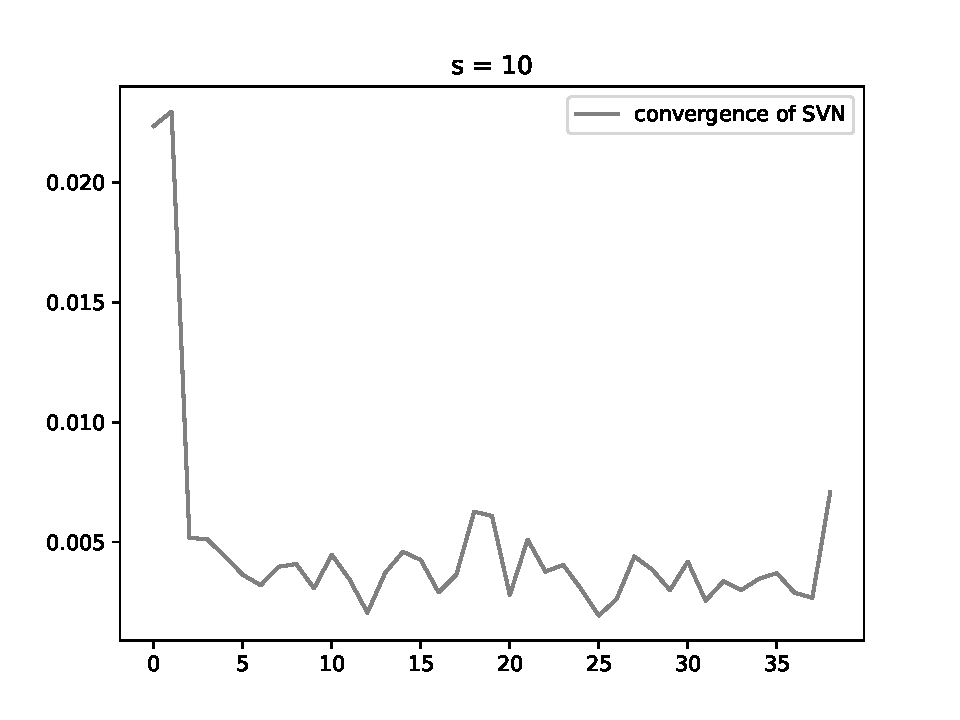
\includegraphics[width=5.5cm]{pics/chapter2/svn-con-1.pdf}
    \captionof{figure}{}
    \end{subfigure}
    \begin{subfigure}[t]{0.3\textwidth}\label{svn-demo2}
    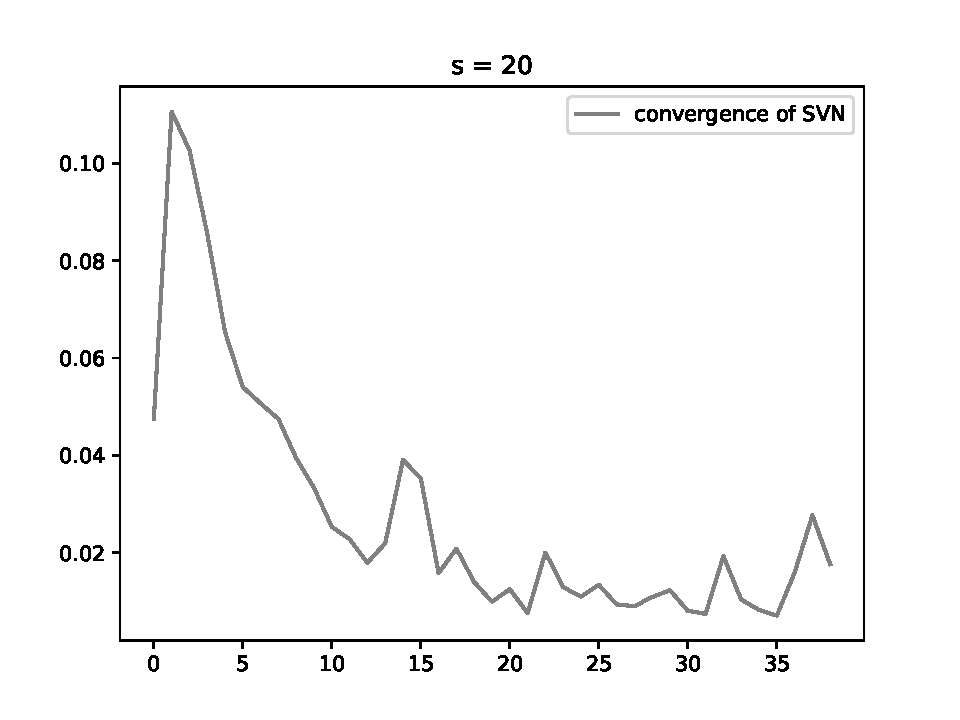
\includegraphics[width=5.5cm]{pics/chapter2/svn-con-2.pdf}
    \captionof{figure}{}
    \end{subfigure}
    \begin{subfigure}[t]{0.3\textwidth}\label{svn-demo3}
    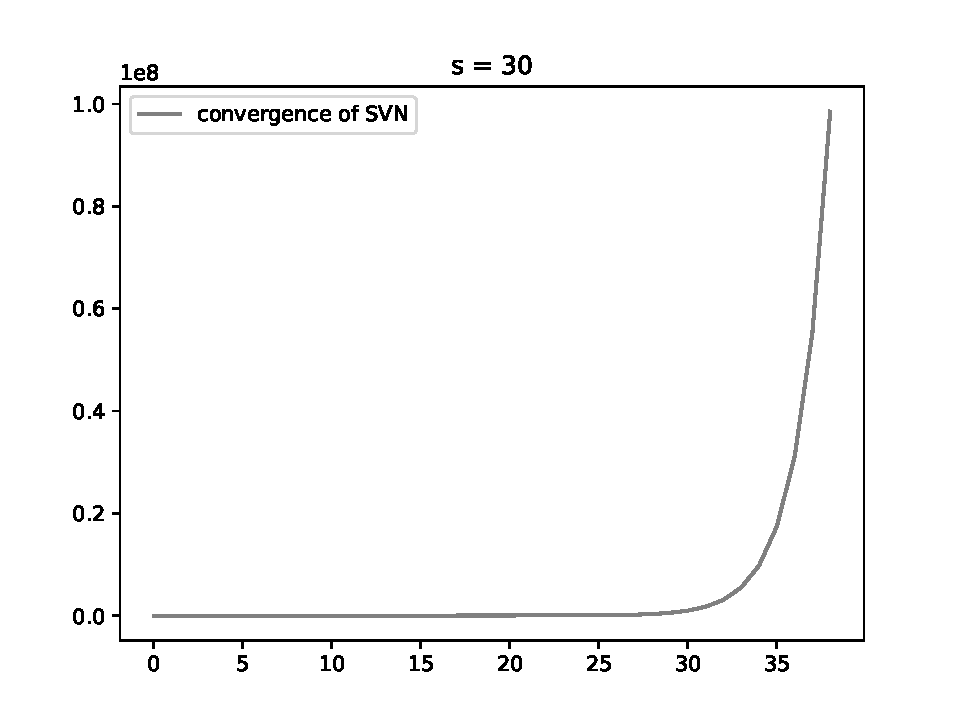
\includegraphics[width=5.5cm]{pics/chapter2/svn-con-3.pdf}
    \captionof{figure}{}
    \end{subfigure}
    \caption{ \small SVN算法的收敛情况}
    \label{svn-demo}
\end{figure}

然而在核密度估计中,一个更大的带宽意味着对该点密度估计包含了更多的样本信息,
选择过很小的带宽,可能造成对核密度估计不准,在应用中需要进行合理选择。

下面我们采用最小二乘估计进行初始化,并且设置终止条件,对算法的性能作进一步的比较。
这次我们将噪声设为正态噪声,但将其中10\%的数据添加柯西噪声,部分性能对比结果见表\ref{perfomance2}。

% Please add the following required packages to your document preamble:
% \usepackage{booktabs}
\begin{table}[H]
    \small
    \caption{部分性能结果对比}\label{perfomance2}
    \resizebox{\textwidth}{!}{
    \begin{tabular}{@{}ccccccccccc@{}}
        \toprule
        s & n     & p   & $\tau$ & Time(SVN) & Time(SVN-full) & Time(LP) & Time(AID) & $l_2$-error(SVN) & $l_2$-error(LS) & $l_2$-error(LP) \\ \midrule
        5 & 20000 & 10  & 12        & 0.12      & 0.42           & 0.17     & 2         & 0.0023        & 0.7304       & 0.0024       \\
        5 & 20000 & 50  & 8         & 1         & 7              & 3        & 13        & 0.0039        & 3.1548       & 0.0020       \\
        5 & 20000 & 100 & 14        & 10        & 28             & 19       & 41        & 0.0059        & 15.0373      & 0.0033       \\
        5 & 20000 & 200 & 27        & 81        & 130            & 170      & 124       & 0.0188        & 151.4039     & 0.0028       \\ 
        5 & 20000 & 500 & 40        & 437        & 437             & 1119       & 698        & 0.0259        & 245.0070      & 0.0026       \\
        \bottomrule
        \end{tabular}
    }
\end{table}
\subsubsection{结论}
AID算法和SVN算法都可以用来求解最小绝对值回归,并且两者在数据规模较大的情况下,都明显快于线性规划。
SVN算法虽然不能保证取得最优解,但是它可以完全避免线性规划计算,因此在计算性能上很有优势;而AID算法
在小规模数据下不具有性能优势,然而在数据集很大时优势明显,并且AID算法最终的解就是对全部数据求解线性规划的结果,
因此它具有更好的稳健性。

我们的结论是,在数据能够服从线性模型时,对最小绝对值回归的计算推荐使用SVN算法,该算法具有很快的速度。
而在一般求解具有$min\ \Sigma_{i=1}^{n} |y_i - \bm{X}_i^T\bm{\beta}|$形式,但是数据能否服从线性模型未知时,
可以先使用最小二乘法拟合,并对模型做出检验然后进行算法选择。对于必须用线性规划来求解的形式类似问题,那么
建议使用AID算法来进行优化。

我们没有进行实验对比带有惩罚项的情况,原因在于:惩罚项主要用来对线性模型中用于系数稀疏化处理,
避免直接拟合的模型具有共线性,在实际应用中普遍使用$L_1$惩罚项。
我们通常已经假定了数据服从线性模型,所以此时SVN算法适用。并且前面提到LASSO算法具有很高的性能,而增加额外约束的线性规划
在速度上就更不具有优势,所以对于带有$L_1$惩罚项的最小绝对值回归,我们始终推荐使用SVN算法。


% \subsection{SVN-AID算法}
% 我们已经研究了AID和SVN两种方法,注意到AID算法的基础思想是具有普适性的。我们不妨再次分析使用AID算法
% 解决最小绝对值回归问题的实质:为了避免在整个数据集上一次性求解,我们使用聚类的方法,希望通过尽可能少的
% 计算来利用样本的信息。不妨将前文提到的AID算法称为AID-LP算法,它成功减少了解决最小绝对值回归问题的LP计算规模。

% 在AID算法求解最小绝对值回归时,
% 假设在第$t$次迭代中我们得到了$\bm{\beta}^{(t)}$,然后根据$\bm{\beta}^{(t)}$对现有的聚类进行拆解。
% 在下一步,我们重新计算该问题,直到达到问题最优解。而$\bm{\beta}^{(t)}$此时已经成功分离了许多聚类,
% 而这些聚类在下一个步骤中仍然全部需要进入计算,因为上一步的参数信息$\bm{\beta}^{(t)}$在下一步计算时被舍弃了。

% 而SVN算法,正是通过利用上一步的参数信息来构造代理变量简化计算。我们不妨结合两种算法的优点,将SVN算法
% 和AID算法结合起来,进一步优化对最小绝对值回归问题的求解。

% \begin{figure}[H]
%     \centering
%     \begin{subfigure}[t]{0.4\textwidth}\label{impro-demo1}
%     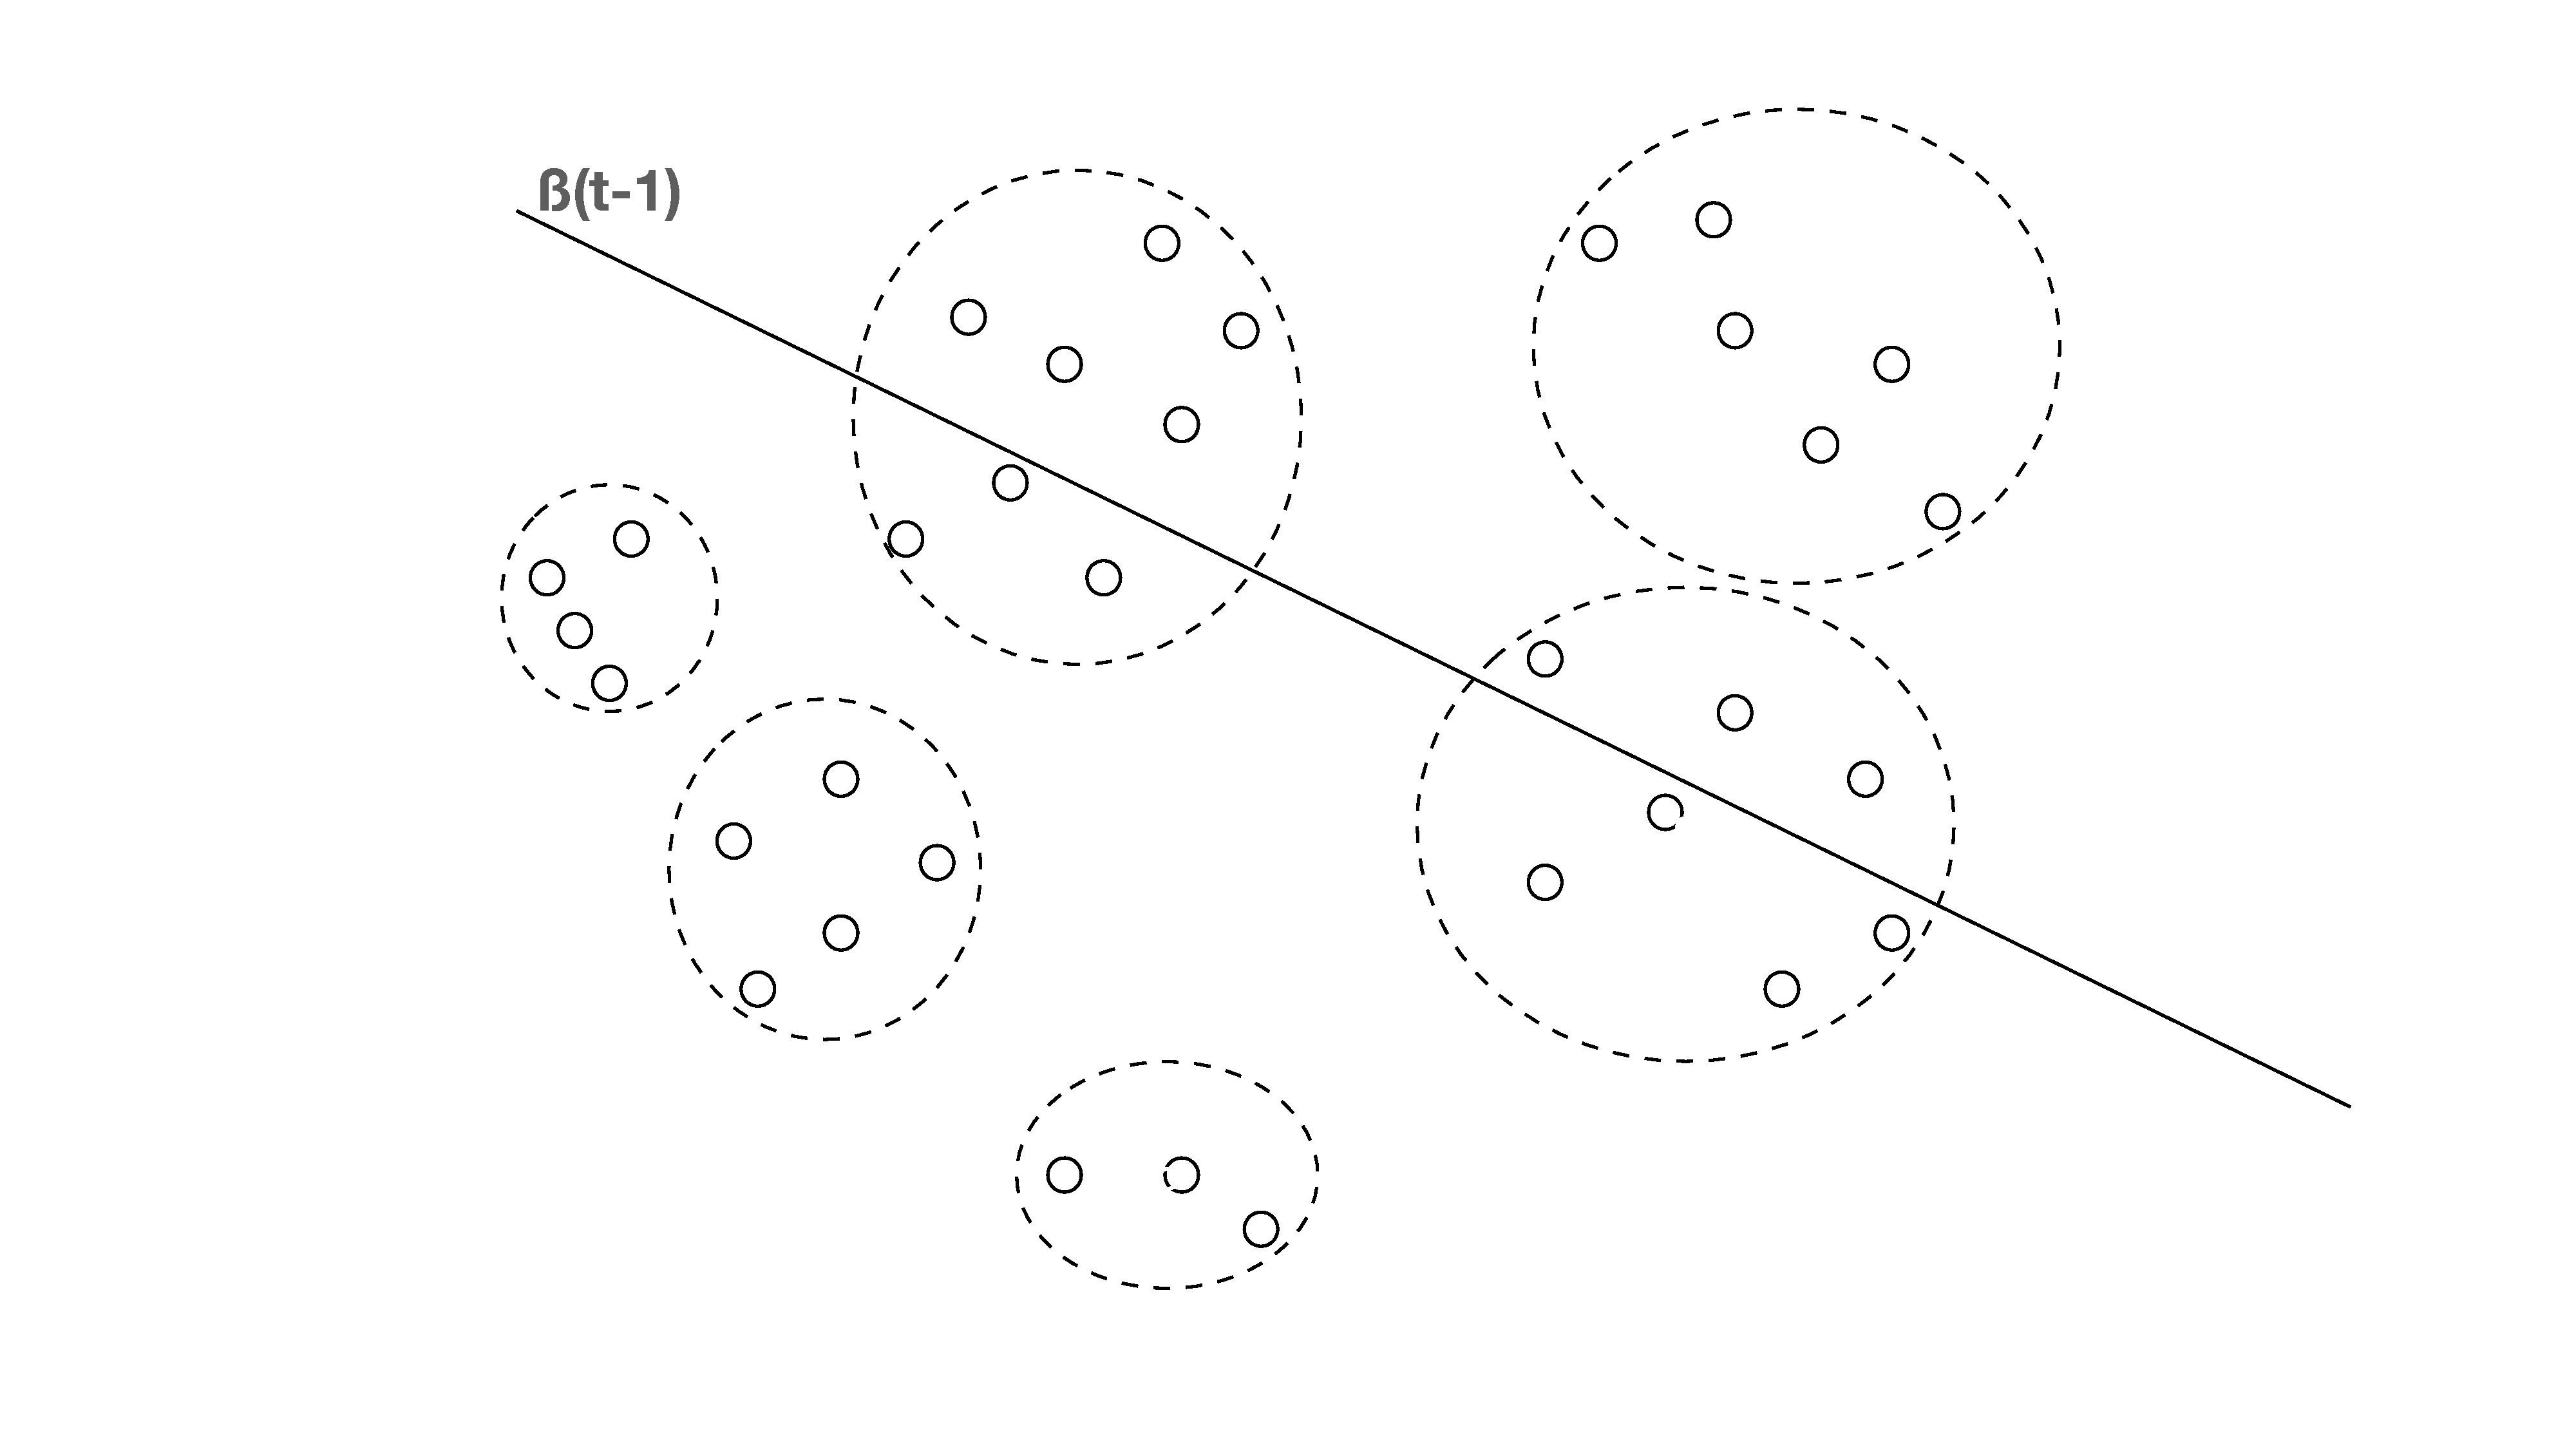
\includegraphics[width=8cm]{pics/chapter2/impro-demo-1.pdf}
%     \captionof{figure}{}
%     \end{subfigure}
%     \centering
%     \begin{subfigure}[t]{0.4\textwidth}\label{impro-demo2}
%     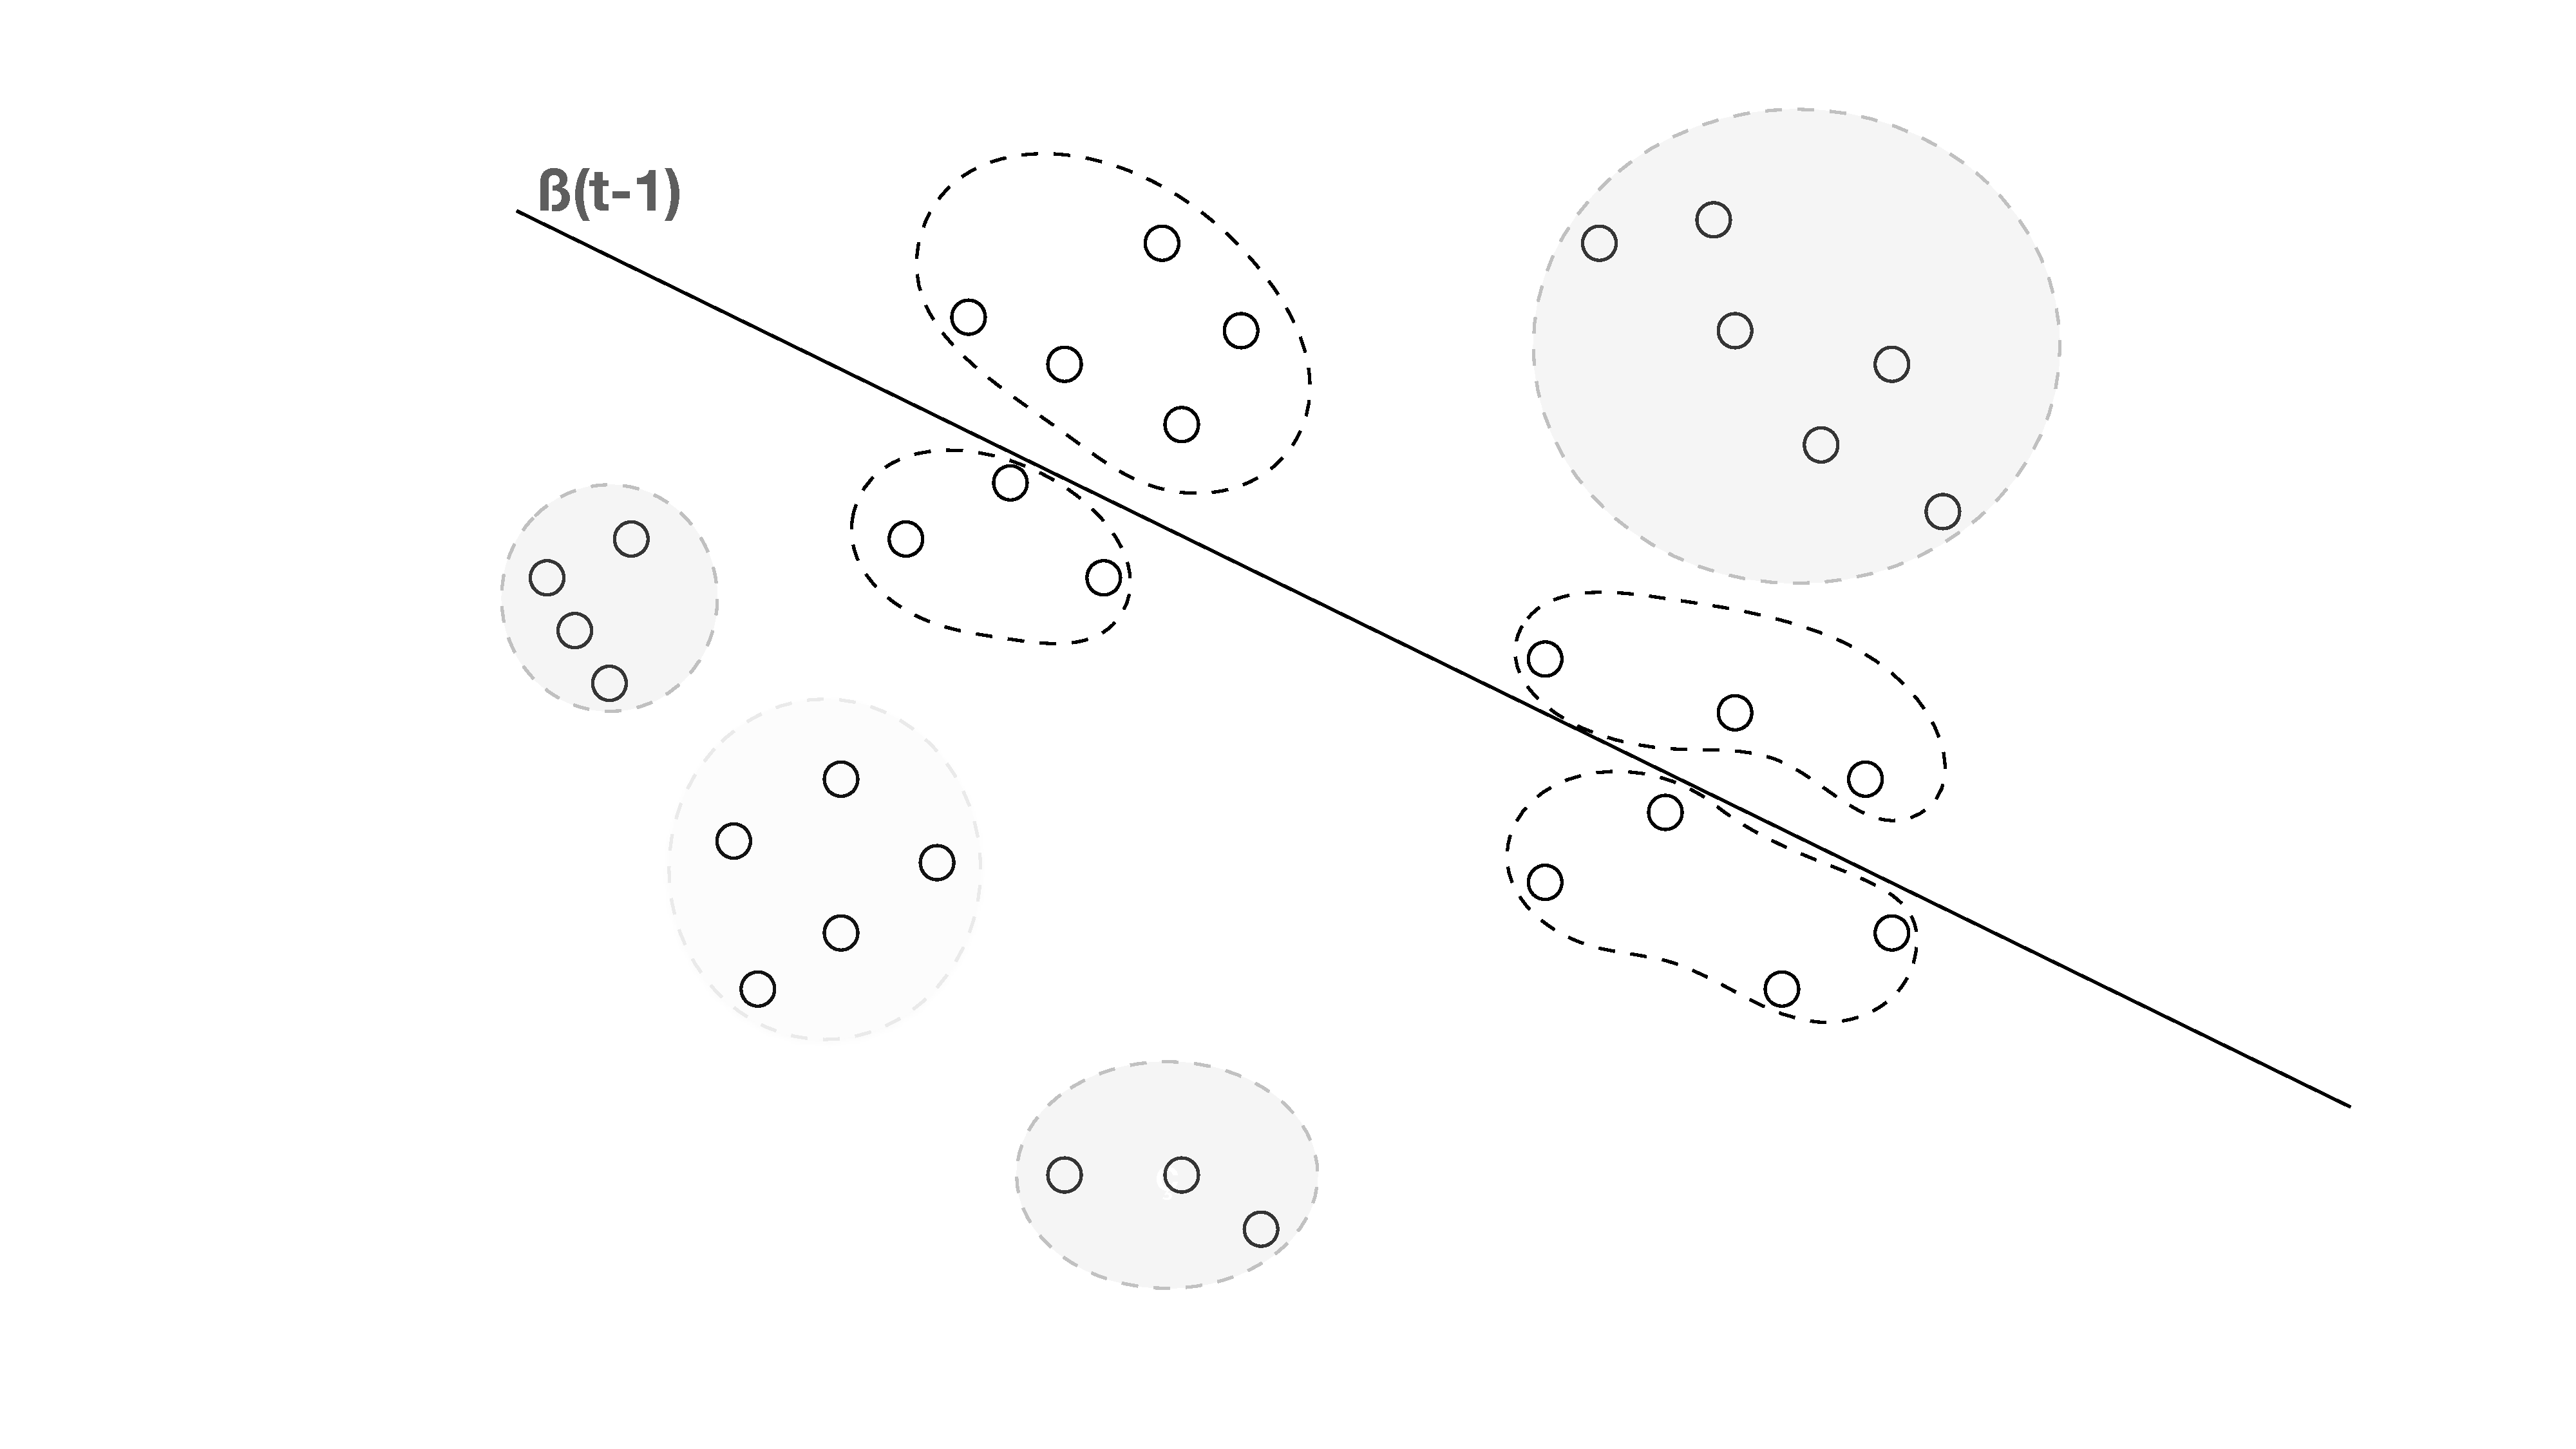
\includegraphics[width=8cm]{pics/chapter2/impro-demo-2.pdf}
%     \captionof{figure}{}
%     \end{subfigure}
%     \caption{ \small SVN-AID算法示意图}
%     \label{impro-demo}
% \end{figure}

% \subsubsection{算法步骤}
% 以下我们给出SVN-AID的步骤:
% 1)初始化:随机采样,进行最小绝对值回归,该步骤使用LP,得到$\hat{\bm{\beta}}^0$。根据各个样本点对该模型的拟合残差进行聚类。
% 2)记上一次迭代得出的系数估计为$\hat{\bm{\beta}}^t$,对当前聚类按照规则拆解。本步骤返回被拆解的聚类组成的集合,
% 舍弃上一步正确分类的聚类。
% 3)根据上一步返回的聚类集合,构造新数据集,并且按照\eqref{svny}构造代理变量数据集,并由\eqref{yl2loss}得出本轮估计。

% 具体见算法3.3,该算法通过舍弃正确分类的聚类,不断缩小问题规模,迭代优化上一步得出的参数估计值来进行对最优解的近似,
% 该算法在理论上可以极大减小AID算法的计算量,并且在舍弃大量样本点的同时,充分利用了前面步骤得出的参数信息。

% \begin{table}[H]%%%%%%开始表格
%     \centering%把表居中
%     \begin{tabular}{{p{0.9\columnwidth}}}%三个c代表该表一共三列,内容全部居中
%     \toprule%第一道横线 表头
%     {\heiti 算法}{\bf 3.3} SVN-AID算法\\
%     \midrule%第二道横线 符号+解释+单位 中间用&隔开
%     输入:$Y$和$\bm{X}$的样本$\bm{Y} = (Y_1, Y_2, ..., Y_n)$,$\bm{X} = (\bm{X}^T_1, \bm{X}^T_2, ..., \bm{X}^T_n)$,
%     迭代次数$\tau$,核函数$K$,依赖于迭代次数的带宽$h^{(t)}$,$(t = 1, ..., \tau)$。
%     \\
%     初始化:给出初始估计,$\hat{\bm{\beta}}^{(0)} $,对每一个样本点$(X_i, Y_i)$根据$Y_i - X_i^T\bm{\beta} $的结果进行
%     K-means聚类,得到聚类结果$C^{(0)} = \{C_1^{(0)}, C_2^{(0)}, ... , C_K^{(0)}\}$。
%     \\
%     对于$t = 1, ..., \tau$:\\
%         1)根据上一轮$\hat{\bm{\beta}}^{(t-1)}$,计算带宽$h^{(t)}$和
%         $\hat{f(0)}^{(t)} = \frac{1}{K^{(t)}h^{(t)}}\sum_{i=1}^{K^{(t)}}K(Y_i - \bm{X}_i^T\hat{\bm{\beta}}^{(t-1)})$。\\
%         据\eqref{svny}在当前聚类上构造替代变量$\tilde{Y} = (\tilde{Y}_1, ..., \tilde{Y}_{K^{(t)}})$;
%         求解
%         $$
%             \hat{\bm{\beta}}^{(t)} = \underset{\bm{\beta} \in \mathbb{R}^{p}}{\operatorname{arg\ min}}
%             \frac1{K^{(t)}} \sum_{k=1}^{K^{(t)}}|C_i^{(t)}|(\tilde{Y}_k - \bm{X}_k^T\bm{\beta})^2
%         $$
%         2)对于$k = 1, ..., K^{(t)}$,计算$\theta_i = y_i - \sum_{j \in J}x_{ij}\hat{\bm{\beta}}_j^{(t)}$,
%         根据$\theta_i$符号异同,将$C^{(t)}_k$分成两个集合,$C_{k+}^{(t)} = \{i \in C_k^{(t)} | \theta_i > 0\}$ ,
%         $C_{k-}^{(t)} = \{i \in C_k^{(t)} | \theta_i < 0\}$,这两个集合在下一步形成新的聚类,
%         即$C^{(t+1)} \leftarrow C^{(t+1)}\bigcup \{ C_{k+}^{(t)}, C_{k-}^{(t)}\}$。 
        
%         输出:$\bm{\beta}^{(\tau)}$
%     \\
%     \bottomrule%第三道横线
%     \end{tabular}
% \end{table}%%%%%%结束表格

% \subsubsection{数值模拟实验}

\subsection{本章小结}

本章首先简要介绍了$L_1$范数的概念,列举了一些其在经济数据分析领域的应用。随后,讨论了
最小绝对值回归的稳健性和其求解方法。

最小绝对值回归已经广泛应用在高维宏观经济数据的处理中,但是它在应用中存在一定的性能问题。
本章介绍了两种可以应用于最小绝对值回归的优化手段:聚类——迭代拆解算法和基于替代变量的估计方法。
进行了数值模拟实验,分析了其优缺点,并给出了其在实际应用中的几点建议。

聚类——迭代拆解算法
是一种非常好的思想,它结合了机器学习中聚类的方法,聚类的作用可以将信息进行提纯,在经过处理
后的数据集上解决原始问题对应的加权优化问题,可以避免直接解决原始问题而耗费庞大的计算量。
聚类——迭代拆解算法可以应用于解决最小绝对值回归问题,它在一定程度上减少了线性规划的计算量,
并且在理论上具有最优解,即它的解一定可以和直接对所有数据求解进行线性规划问题一样好。

另外,本章介绍了另外一种巧妙的算法——一种基于替代变量的迭代算法,该算法通过
构造替代变量,从而将原来需要通过线性规划解决的最小绝对值回归问题转化为
解决替代变量的最小二乘问题。这样一来,计算的复杂度就大大降低。该方法在
实际应用中性能表现十分优秀,但是需要注意带宽的选择。

聚类——迭代拆解算法对和最小绝对值回归目标函数相同的任何优化问题均适用;
然而SVN算法在其理论基础上需要假设线性模型成立,需要结合我们面临的实际问题酌情使用。

最后,我们在本章对最小绝对值回归性能优化的研究,会对后续
章节中优化$L_1$范数主成分分析法估计近似因子模型的求解算法有推动作用。

   \section{因子模型的$L_1$范数主成分估计算法研究}

本章继续讨论$L_1$范数主成分分析,重点在于讨论$L_1$主成分分析的求解算法。
$L_1$主成分分析虽然在稳健性上有很大优势,但是其求解需要比$L_2$主成分分析
多得多的时间,在很多场合下限制了它的应用。

在第\ref{chapter3}中的研究中,已经重点讨论了优化最小绝对值回归的算法,
注意到交替凸优化算法中包含了最小绝对值回归问题,
因此可以充分利用得出的结论,尝试将两种算法应用于改良交替凸优化算法。
之后通过一个模拟实验和对一个高频金融数据的主成分分析的测试,
测试了算法的性能。

至此我们已经对问题$P_3$做出了较为深入的讨论,而问题$P_4$同样值得探究,它是$L_1$主成分分析的另一重要研究方向。
我们将介绍一种利用贪婪策略求解$P_4$算法,并通过模拟实验证明算法的有效性。

在第\ref{chapter2}章,我们将交替凸优化算法用于近似因子模型的估计,并且通过实证研究论证了
$L_1$范数主成分分析得出的因子同样适用于宏观经济预测中,并且有良好的预测表现。
本章的最后,我们将求解$P_4$来得到的因子估计量同样在国内主要月度宏观经济数据预测场景下进行了测试,
并给出了一些结论与建议。

\subsection{改进的$L_1$主成分分析交替凸优化算法}
在第\ref{chapter2}章中,我们提出了求解$L_1$主成分分析的交替凸优化算法;
交替凸优化算法的计算量主要集中在\eqref{subpro}和\eqref{subproabs},注意到
在数据服从因子模型的假设下,\eqref{subproabs}是一个最小绝对值回归问题。
因此我们可以尝试使用第\ref{chapter3}章中基于替代变量的估计算法来代替线性规划求解\eqref{subproabs}。

\subsubsection{基于替代变量算法的交替凸优化算法改进}
前文我们已经讨论了一种基于替代变量的估计算法,该算法在求解最小绝对值回归时具有较好的性能提升效果。
在前文已经阐述了该算法的理论基础,注意到\eqref{rho-problem}与\eqref{randomversion}关联起来的前提是线性模型成立。
即需要保证$\mathbb E(Y|\bm{X}^T\bm{\beta})$必须存在。

改写\eqref{subproabs},
\begin{equation}
    \bm a_i = \underset{\bm {\theta}}{\operatorname{arg\ min}} \sum_{j=1}^n |x_{ij} -\bm{\theta}^Tf_j|
\end{equation}
假设数据服从因子模型,可认为$\mathbb E (\bm X|\bm{f})$存在,因此这里\eqref{subproabs}为一最小绝对值回归问题。

下面给出使用基于替代变量的估计算法改进交替凸优化算法的步骤。
\begin{table}[H]%%%%%%开始表格
    \centering%把表居中
    \begin{tabular}{{p{0.9\columnwidth}}}%三个c代表该表一共三列,内容全部居中
    
    \toprule%第一道横线 表头
    算法4.1:基于替代变量算法改进的交替凸优化算法(ACP-SVN) \\
    \midrule%第二道横线 符号+解释+单位 中间用&隔开
    1.初始化:给出$\bm{A}$,$\Sigma$的初始值$\bm{A}^{(0)}$,这里我们始终采用$L_2$主成分估计的因子载荷矩阵作为初始估计
    ,$\Sigma^{(0)} = I$,(其中$\Sigma$为一对角矩阵,
    $I$为单位矩阵); \\

    2.交替凸优化:对于迭代次数$t = 1, ..., T$: \\
    $$p_1:\ F^{(t)} = \underset{F}{\operatorname{arg\ min}} \|X - \bm{A}^{(t-1)}\Sigma^{t-1}F^{T}\|_{L_1}$$ \\
    $$p_2:\ \bm{A}^{(t)} = \underset{\bm{A}}{\operatorname{arg\ min}} \|X - \bm{A}\Sigma^{t-1}F^{Tt} \|_{L_1}$$ \\
    $p_1$对应的若干子问题,采用线性规划法求解;$p_2$对应的若干子问题,采用SVN算法求解\\
    \begin{equation*}
        \text{归一化:}\left\{
                    \begin{array}{clr}
                    N_a = diag(\bm{A}^{tT}\bm{A}^{t})\\
                    N_f = diag(F^{Tt}F^{t})\\
                    F^{t} \leftarrow F^{t}N_f^{-1}\\
                    \bm{A}^{t}\leftarrow \bm{A}^{t}N_a^{-1}\\
                    \Sigma^{t} \leftarrow N_a\Sigma^{t-1}N_f\\
                    \end{array}
        \right.
    \end{equation*} \\

    3.输出结果:$\bm{A} \leftarrow \bm{A}^T\Sigma^{1/2}$,对$\bm{A}$进行QR分解取正交矩阵得到$\hat{\bm{A}}$;
    $\hat{\bm{F}} \leftarrow \hat{\bm{A}}^T\bm{X}$。
     \\
    \bottomrule%第三道横线
    \end{tabular}
\end{table}%%%%%%结束表格

\subsubsection{基于聚类——迭代拆解算法的交替凸优化算法改进}
上面我们给出了在因子模型假设下交替凸优化的算法改进。
然而对于人脸图像数据的主成分分析、带有噪声的信号数据的主成分分析等情形,
因子模型往往不成立,此时
我们需要寻找更加通用的优化手段。

我们可以尝试使用聚类——迭代拆解算法求解\eqref{subproabs}和\eqref{subpro},
做法是采用聚类——迭代拆解算法对交替每一个子问题进行求解,其余具体步骤同算法2.1。

\subsubsection{数值模拟}
为了对改进后的算法性能进行测试,首先进行数值模拟。这里
我们模拟一个高维的因子模型,用来对比三种方法的求解性能。

令$\bm{f} = (f_1, ..., f_m)$为一$m$维随机变量,服从$N(\bm{0}, \bm{I}_m)$。
根据模型\eqref{orth-factor},为模拟$(X_1, ..., X_p)$,首先随机产生$p\times m$的因子载荷矩阵,
之后产生$\bm{f}$的$n$组随机取值,并求出观测变量的对应观测值矩阵$\bm X $。
最后随机取$10\%$的观测,加上柯西噪声。

取不同的$(m, p, n)$来测试三种算法的性能表现,
我们记录每次取值下算法运行的CPU时间和重构误差(这里就是因子残差)平方的中位数。
部分性能比较结果见\ref{three-l1-pca}
(需要注意本实验是在低功耗便携式计算机上,采用Python脚本测试的。
即使如此,每次实验的时间也和交替凸优化算法的迭代终止条件的选取以及算法实现的方式有很大关联,
本实验的性能结果并不代表交替凸优化算法
标准实现的性能,事实上已经存在一些良好的C++实现,计算性能比我们编写的Python程序要快得多。
另外本实验中$\alpha = 1\times10^{-12}$)
,其中$L_2$主成分分析的因子残差平方中位数也列出。

\begin{table}[H]
    \small
    \centering
    \caption{三种算法的比较结果}
    \label{three-l1-pca}
    \begin{tabular}{@{}cccccccccc@{}}
    \toprule
       &      &     & \multicolumn{2}{c}{ACP} & \multicolumn{2}{c}{ACP-SVN} & \multicolumn{2}{c}{ACP-AID} & PCA-L2   \\ \midrule
    m  & n    & p   & Time     & l2-error     & Time       & l2-error       & Time       & l2-error       & l2-error \\ \midrule
    5  & 1000  & 50  & 47       & 0.0083       & 19         & 0.0115         & 129        & 0.0083         & 0.39     \\
    10 & 1000  & 50  & 68       & 0.0064       & 17         & 0.0096         & 104        & 0.0064         & 0.58     \\
    5  & 5000 & 50  & 119      & 0.0382       & 31         & 0.1232         & 278        & 0.0382         & 1.24     \\
    10 & 5000 & 50  & 107      & 0.0259       & 79         & 0.1352         & 321        & 0.0259         & 0.85     \\
    5  & 5000 & 100 & 689      & 0.0725       & 362        & 0.1480         & 1782       & 0.0725         & 1.26     \\
    10 & 5000 & 100 & 792      & 0.0664       & 510        & 0.2394         & 1440       & 0.0664         & 2.99     \\
    5  & 2000  & 200 & 3567     & 0.0992       & 1135       & 0.4903         & 3290       & 0.0992         & 2.07     \\
    10 & 2000  & 200 & 3893     & 0.1033       & 1650       & 0.5790         & 5033       & 0.1033         & 3.12     \\ \bottomrule
    \end{tabular}
\end{table}

从结果中我们发现,ACP-SVN算法的性能优势较为明显,而ACP-AID算法的性能表现则相对一般,并没有明显的改进效果。而理论上说,
两者都应该在数据规模较大的情况下有明显的提升,局限于本次实验平台的计算能力,我们把更多的测试留到今后的进一步研究中。


\subsection{求解特征空间$L_1$范数最大化的贪婪算法}

我们已经在第三章中研究了$P_3$,这里我们首选给出问题$P_4$的规范化表述:
\begin{equation}\label{p4}
    P_4: \ \hat{\bm A} = \underset{\bm{A}}{\operatorname{arg \ max}} \| \bm A^T \bm X\|_{L_1}
    = \underset{\bm A}{\operatorname{arg\ max}} 
    \sum_{i=1}^{n}\sum_{k=1}^{m}|\sum_{j=1}^p{a}_{jk}x_{ij}|
     \text{,其中}\bm A^T\bm A = \bm I_m
\end{equation}

这里我们介绍一种求解$P_4$的算法。求解\ref{p4}时,
由于对于不同的$m$,最优$\bm a_j^*$会发生变化,因此想要得出\ref{p4}的全局最优解是非常复杂的。
下面介绍Kwak于2008年提出的一种算法\cite{kwak2008principal},它将问题分解一个个$m=1$的子问题,然后用贪婪策略获得全局解。
该算法直观、简洁并且易于实现。
\subsubsection{求解子问题}

首先考虑$m = 1$的情况,该问题寻找\eqref{m-1}的最优解。
\begin{equation}\label{m-1}
    \bm a^* = \underset{\bm a}{\operatorname{arg\ max}}\| \bm a ^T \bm{X}\|_{L_1}
    = \underset{\bm a}{\operatorname{arg\ max}}\sum_{i=1}^n|\bm a^T\bm x_i|
    \text{,其中}\|\bm a\|_{L_2} = 1
\end{equation}

算法4.2给出了\eqref{m-1}的求解算法。
\begin{table}[H]%%%%%%开始表格
    \centering%把表居中
    \begin{tabular}{{p{0.9\columnwidth}}}%三个c代表该表一共三列,内容全部居中
    
    \toprule%第一道横线 表头
    算法4.2 $m=1$时的$P_4$求解算法\\
    \midrule%第二道横线 符号+解释+单位 中间用&隔开
        初始化:取$\bm a$的任意初始值;$\bm a^0\leftarrow \bm a^0/\|a^0\|$。 \\
        对于$t = 1, ..., T$:\\
            1.对所有的$i \in \{1, ..., n\}$,若$\bm a^{0T}\bm x_i < 0$,令
            $p_i^t = -1 $,否则$p_i^t = 1$ 。\\
            2.令$t \leftarrow t+1$并且$\bm a^t = \sum_{i=1}^np_i^{t-1}\bm x_i$;
            $\bm a^t \leftarrow \bm a^t/ \|\bm a^t\|_{L_2}$ 。\\
            3.检查是否收敛:\\
            1)如果$\bm a^t \neq \bm a^{t-1}$,回到步骤2;\\
            2)若存在某个$i$使得$\bm a^T\bm x_i = 0$,令$\bm a^t \leftarrow
            (\bm a^t + \Delta \bm a)/\|\bm a^t + \Delta \bm a\|_{L_2}$并回到步骤2,这里
            $\Delta \bm a$为一个很小的随机向量; \\
            3)若前面两个都不符合,令$\bm a^* = \bm a^t$,算法返回。\\
    \bottomrule%第三道横线
    \end{tabular}
\end{table}%%%%%%结束表格
按照算法4.2得出的$\bm a^*$是$\bm x_1, ..., \bm x_i$的线性组合,即$\bm a^t \propto \sum_{i=1}^np_i^{t-1}\bm x_i$,
故其拥有旋转不变性。注意到的$a^*$为\eqref{m-1}的最优解,它可能不是\eqref{p4}的全局最优解。
$\bm a^0$可以任意设置,因此可以采用$L_2$主成分作为其初始值,从而提高解趋向全局最优的可能性。

\subsubsection{贪婪策略求解主成分}
前文已经给出了获得$m = 1$时$P_4$最优解的算法,我们可以通过贪婪策略来求解$P_4$。贪婪策略是一种
在问题的动态求解过程中,对问题所处的每一个当前状态都寻求其最优解,从而期望能够逼近全局最优解的算法设计思想。
下面给出利用贪婪策略求解$P_4$的步骤,
\begin{table}[H]%%%%%%开始表格
    \centering%把表居中
    \begin{tabular}{{p{0.9\columnwidth}}}%三个c代表该表一共三列,内容全部居中
    
    \toprule%第一道横线 表头
    算法4.3:求解特征空间$L_1$范数最大化的贪婪算法\\
    \midrule%第二道横线 符号+解释+单位 中间用&隔开
        输入:$\bm a^0$,$\{\bm x_i^0 = \bm x_i\}_{i=1}^n$。\\
        对于$j = 1, ..., m$: \\
        对所有的$i \in \{ 1, ..., n\}$,$\bm x_i^j = x_i^{j-1} - \bm a^{j-1}(\bm {a^{(j-1)T}}\bm x_i^{j-1})$ , \\
        通过算法4.2求解$\bm a^j$,令$\bm{X}^j = [\bm x_1^j, \bm x_2^j, ..., \bm x_i^j]$。 \\
    \bottomrule%第三道横线
    \end{tabular}
\end{table}%%%%%%结束表格

\subsubsection{模拟与实证}
参考\ref{lab-1}中的实验,我们首先测试该方法是否同样能够获得稳健的$L_1$主成分,
对照交替凸优化算法和$L_2$主成分分析的结果,我们发现求解$P_4$同样可以获得很好的
重构表现。
我们的结论是$P_4$同样可以作为稳健主成分分析的手段,适合处理带有大量离群值的数据。

需要注意的是由于$P_3$和$P_4$并不是一组对偶问题,它们求解获得的主成分是不同的。
前文已经通过实证研究发现,$P_3$求解获得的主成分可以作为因子模型的主成分估计,
并且在扩散指数模型中拥有良好的预测表现。
这里我们同样基于国内月度宏观经济数据对算法4.2进行测试,将得到的$L_1$主成分
作为扩散指数模型的因子得分对部分指标进行经济预测。

我们列出一些在第\ref{chapter2}中展示的经济指标预测情况,部分结果见表\ref{outcome4}至表\ref{outcome6},
注意其中PCA L1代表因子得分使用算法4.2估计。

\begin{table}[H]
    \centering
    \small
    \caption{向前一个月预测结果}
    \label{outcome4}
    \begin{tabularx}{\textwidth}{lXXXXXX}
    \toprule
                 &  MSE(L1 PCA) &  MSE(PCA L1) &  MAE(L1 PCA) &  MAE(PCA L1) &  MPAE(L1 PCA) &  MPAE(PCA L1) \\ \midrule
    消费者满意指数     & 0.81            & 0.78        & 0.87            & 0.83        & 0.43             & 0.67         \\
    工业生产者出厂价格指数 & 0.70            & 0.83        & 0.75            & 0.92       & 0.96             & 0.90         \\
    货币供应量M2      & 0.76            & 1.01        & 0.90            & 1.00       & 0.45             & 0.92         \\
    固定资产投资总额  & 0.89            & 1.11        & 0.97            & 1.03        & 0.81             & 1.05         \\
    房地产开发投资总额 & 0.79            & 0.94        & 0.95            & 0.97        & 0.91             & 1.10         \\
    社会消费品零售总额 & 0.84            & 0.62        & 0.87            & 0.78        & 0.45             & 0.76         \\
    制造业采购经理指数    & 1.24            & 0.99        & 1.06            & 1.14        & 0.90             & 0.82         \\
    住宅新开工面积总数  & 0.89            & 1.20        & 0.85            & 1.12        & 0.45             & 1.19         \\
    股票流通市值     & 0.99            & 1.23        & 0.98            & 1.12        & 0.81             & 0.98         \\
    消费者信心指数     & 0.93            & 0.70        & 0.98            & 0.80        & 0.98             & 0.99         \\ \bottomrule
    \end{tabularx}
\end{table}

\begin{table}[H]
    \centering
    \small
    \caption{向前三个月预测结果}
    \label{outcome5}
    \begin{tabularx}{\textwidth}{lXXXXXX}
    \toprule
                 &  MSE(L1 PCA) &  MSE(PCA L1) &  MAE(L1 PCA) &  MAE(PCA L1) &  MPAE(L1 PCA) &  MPAE(PCA L1) \\ \midrule
                 消费者满意指数    & 0.85            & 1.16        & 0.95            & 1.22        & 1.32             & 0.78         \\
    工业生产者出厂价格指数& 0.98            & 0.88        & 0.97            & 0.93        & 0.93             & 0.97         \\
    货币供应量M2       & 1.08            & 0.59        & 1.05            & 0.71        & 0.66             & 0.70         \\
    固定资产投资总额  & 0.99            & 1.03        & 0.98            & 1.06       & 0.82             & 0.90         \\
    房地产开发投资总额 & 0.91            & 0.97        & 0.92            & 1.00       & 0.66             & 0.89         \\
    社会消费品零售总额 & 0.62            & 1.48        & 0.85            & 1.24        & 1.26             & 1.50        \\
    制造业采购经理指数    & 1.26            & 0.90        & 1.10            & 0.93        & 1.04             & 0.87         \\
    住宅新开工面积总数   & 0.81            & 0.75        & 1.12            & 0.89        & 1.04             & 0.90         \\
    股票流通市值   & 0.99            & 1.44        & 1.00            & 1.31        & 1.04             & 1.22         \\
    消费者信心指数    & 0.99            & 1.12        & 0.96            & 1.00        & 0.94             & 1.03         \\ \bottomrule
    \end{tabularx}
\end{table}

\begin{table}[H]\label{outcome3}
    \centering
    \small
    \caption{向前六个月预测结果}
    \label{outcome6}
    \begin{tabularx}{\textwidth}{lXXXXXX}
    \toprule
                 &  MSE(L1 PCA) &  MSE(PCA L1) &  MAE(L1 PCA) &  MAE(PCA L1) &  MPAE(L1 PCA) &  MPAE(PCA L1) \\ \midrule
                 消费者满意指数     & 0.91            & 1.00        & 0.93            & 1.00        & 0.68             & 0.99         \\
    工业生产者出厂价格指数 & 1.00            & 1.40        & 0.94            & 1.19        & 0.79             & 1.28         \\
    货币供应量M2      & 0.84            & 0.99        & 1.06            & 1.00        & 1.46             & 1.04         \\
    固定资产投资总额  & 0.88            & 0.69        & 0.94            & 0.73        & 0.93             & 0.85         \\
    房地产开发投资总额 & 0.90            & 0.58       & 0.91            & 0.67        & 0.73             & 0.79        \\
    社会消费品零售总额 & 0.64            & 1.36        & 0.79            & 1.14        & 1.30             & 1.45         \\
    制造业采购经理指数   & 1.46            & 1.20        & 1.20            & 1.09        & 1.45             & 1.42         \\
    住宅新开工面积总数  & 0.85            & 0.83        & 0.96            & 0.92        & 0.70             & 0.69        \\
    股票流通市值   & 0.98            & 1.20        & 1.01            & 1.16        & 1.28             & 0.97         \\
    消费者信心指数     & 0.99            & 1.07        & 0.98            & 1.00        & 0.97             & 0.87         \\ \bottomrule
    \end{tabularx}
\end{table}

\subsection{本章小结}
本章进一步讨论了$L_1$范数主成分分析的求解算法问题。
首先我们结合上一章的研究内容,结合交替凸优化算法的特点,
对其涉及最小绝对值回归的步骤做出了改进。通过一个因子模型
数据的模拟实验,我们比较了改进后的算法的性能。由于实验平台
计算能力的限制,我们的实验结果稍显不够详尽。
然而实验结果已经能够发现,在对因子模型进行$L_1$主成分估计的
场合,我们对交替凸优化算法的改进尝试是有明显效果的。

另外针对$L_1$范数主成分分析的另一种求解思路,
我们也介绍了实现的经典算法。通过模拟实验和实证,
证明了两种$L_1$范数主成分分析的求解都具有很好的稳健性,
并且同样适用于扩散因子模型进行宏观经济预测。


   \section{总结与展望}


\subsection{研究成果总结}
$L_1$范数主成分分析比传统主成分分析更加稳健可靠,使用$L_1$主成分分析可以进行更加稳健的因子模型估计
从而更好地进行宏观经济分析和预测。本文围绕相关问题展开了理论与实证研究,并取得如下成果:

1)扩散指数模型可以利用高维宏观经济变量的静态因子作为预测变量来进行有效的宏观经济预测。
本文创新性地将$L_1$主成分分析应用于静态因子的估计中,实证研究表明:$L_1$主成分分析估计得到的因子
具有良好的预测效果,并且更具稳健性和准确性。

2)交替凸优化算法是求解$L_1$主成分分析的经典算法,然而其在计算效率上较慢。本文
首先研究了最小绝对值回归的两种优化求解算法,并且结合两者进行了一定的创新。之后我们将
优化的最小绝对值回归求解算法应用于交替凸优化算法中,代替线性规划,获得了更高的计算效率。

3)最后,$L_1$主成分分析根据问题不同有不同的求解方式。我们对两种不同求解算法都进行了介绍,并通过
模拟与实证研究,论证了两种方法都可以对因子模型进行稳健的估计,在宏观经济预测中更具稳健性和准确性。

\subsection{不足与展望}
我们虽然已经对求解$L_1$主成分分析的交替凸优化算法进行了优化尝试,
但是在规模很大的数据场景下,其
计算时间仍然不可接受。
在数据满足因子模型时,我们的优化尝试更加有效些,然而我们的方法依旧不易处理高维数据($p >> n$)的问题。

自$L_1$主成分分析提出,不断有新的求解
算法被开发出来,然而至今没有算法可以求解问题$P_3$的最优解,并且维数和观测都很大的$P_4$问题已经被证明
为NP难题。
因此,继续深入探究$P_3$的求解算法,推广$L_1$范数主成分分析的应用就成了我们下一步的
研究愿景。

国外学者已经在实证研究中大量应用因子模型,其中包括了应用于混频数据和高维数据进行经济短期预测和
实时预测的研究。我们希望在后续的研究中,能够涉及因子模型更加丰富的应用场景,
对$L_1$主成分估计的应用价值做更多的发掘。

最后,我们知道$L_1$范数主成分分析问题的两种形式对应了两种不同的解,而本文并未对最优解的统计性质
做理论上的探究。在后续研究中,深入探讨相关理论也将是重要的目标。


   % \addcontentsline{toc}{section}{参考文献}%将“参考文献加入目录中”
   % \printbibliography
   % \addcontentsline{toc}{section}{附录}
   % \centerline{\large\heiti 附\ 录 }

\vspace{2ex}
{\heiti\large A.\ 作者在攻读硕士学位期间发表论文及所获奖项}

{\heiti 已录用文章\ [第二作者]} \ 孔新兵,蒯强,汪红霞. 高维$L_1$稳健因子分析及其在宏观经济预测中的应用.吉林工商学院学报,2019.

{\heiti 所获奖项\ [指导者:王江艳]}. 2020年全国应用统计研究生案例大赛,二等奖。
\thispagestyle{plain}

   % \addcontentsline{toc}{section}{后记}
   % \centerline{\large\heiti 后\ 记}

\vspace{2ex}

时光荏苒,我已在南京审计大学度过了三个年头,在统计与数学学院的研究生生涯也已接近尾声。
在南京审计大学的这段读书时光,注定会是我一生中的宝贵记忆。

在毕业论文完成之际,首先要感谢我的导师孔新兵教授。跟老师相处的三年时光下来,我被老师
渊博的专业知识、严谨的治学风格和平易近人的学者风范所深深感染。毕业论文的顺利完成,离不开
老师的悉心指导和耐心修改,从选题到最终的定稿,老师都给予了耐心的指导,帮助我解决
撰写过程中的诸多难题。
三年来,在孔新兵老师的指导下我对所学专业有了更深层次的认识,为学为人方面都有了很大进步。
临近毕业,我已有了一定的知识储备和实习经验,即将走上工作岗位,老师的谆谆教诲,
我会铭记在心。在今后漫长的工作生涯中,我还会不断向老师继续请教和学习。

另外,感谢南京审计大学和统计与数学学院给我的培养机会。我本科并不是相关专业,
后由于各种机遇来到南审,进行应用经济学统计学方向的学习和研究,这对我的知识面是极大的
拓宽,这三年的学习经历对我今后的终身学习具有莫大的帮助。
毕业后我将从事软件开发工作,随着岁月的流逝,我可能会忘记在学校学习过的一些课程,可能会
记不起一些教授过我课程的老师。但是在这三年中,学校和学院老师们脚踏实地的
态度和积极乐观的性格将默默影响我今后的成长。

另外,感谢和我朝夕相处的研究生同学们。感谢他们在我专业基础薄弱时给予的耐心帮助以及
一起参加学科竞赛时大家的合作无间。三年的时间很快就过去了,
我的性格也变得更加成熟,认识了越来越多的朋友。每一位同学身上都有太多值得我学习的地方,
毕业只是我们学生生涯的结束,与各位同学的宝贵友谊将会伴随我们终身。

最后,感谢学校和学院给我们安排评阅论文的各位专家、教授,感谢各位提出的宝贵意见,
使得我的论文更加完善。
\vspace{2ex}

\rightline{ 蒯强\ \ \ \ \ }
\vspace{1ex}
\rightline{2021年5月 }
\end{document}